\documentclass[a4paper,oneside,english,brazil,11pt,a4paper,openright,titlepage,usenames,dvipsnames]{book}
\usepackage[T1]{fontenc}
\usepackage[utf8]{inputenc}
\usepackage{lmodern}
\setcounter{secnumdepth}{3}
\setcounter{tocdepth}{3}
\usepackage{array}
\usepackage{verbatim}
\usepackage{calc}
\usepackage{graphicx}
\usepackage{textcomp}
\usepackage{listings}

%PDF table of contents
\usepackage{hyperref}
\hypersetup{pdftex,colorlinks=true,allcolors=blue}
\usepackage{hypcap}
% -------------------

\makeatletter

%%%%%%%%%%%%%%%%%%%%%%%%%%%%%% LyX specific LaTeX commands.
\pdfpageheight\paperheight
\pdfpagewidth\paperwidth

%% Because html converters don't know tabularnewline
\providecommand{\tabularnewline}{\\}

%%%%%%%%%%%%%%%%%%%%%%%%%%%%%% User specified LaTeX commands.
% Classe alternativa, apropriada para impressão frente-verso. Inclui páginas em branco
% de forma que capítulos sempre tenham início na página à direita:
% \documentclass[11pt,a4paper,openright,titlepage]{book}

% Pacotes
\usepackage[brazilian]{babel}
\usepackage{epsfig}
\usepackage{subfigure}
\usepackage{amsfonts}
\usepackage{amsmath}
\usepackage[thmmarks,amsmath]{ntheorem}%\usepackage{amsthm}
\usepackage{boxedminipage}
\usepackage{geometry}
\usepackage{theorem}
\usepackage{fancybox}
\usepackage{fancyhdr}
\usepackage{ifthen}
\usepackage{url}
\usepackage{afterpage}
\usepackage{color}
\usepackage{colortbl}
\usepackage{rotating}
\usepackage{makeidx}
\usepackage{indentfirst}
% Pacotes para adiçao de figuras do inkscape
\usepackage{graphicx}
\usepackage{import}
%\usepackage[usenames,dvipsnames]{color}

\usepackage{tikz}
\usetikzlibrary{positioning}
\usepackage{textcomp}
\usepackage{tabularx}
\usetikzlibrary{shapes,arrows}

% Escolher um dos seguintes formatos:
%\usepackage{ft1unb} % segue padrão de fonte Times
\usepackage{ft2unb} % segue padrão de fontes do Latex

\makeindex
% Added by lyx2lyx
\usepackage{amssymb}

\makeatother

\usepackage{babel}

\usepackage{beramono}
\usepackage{listingsutf8}
%\usepackage[usenames,dvipsnames]{xcolor}

%%
%% Julia definition (c) 2014 Jubobs
%%
\lstdefinelanguage{Julia}%
  {morekeywords={abstract,break,case,catch,const,continue,do,else,elseif,%
      end,export,false,for,function,immutable,import,importall,if,in,%
      macro,module,otherwise,quote,return,switch,true,try,type,typealias,%
      using,while},%
   sensitive=true,%
   alsoother={\$},%
   morecomment=[l]\#,%
   morecomment=[n]{\#=}{=\#},%
   morestring=[s]{"}{"},%
   morestring=[m]{'}{'},%
}[keywords,comments,strings]%

\lstset{%
    language         = Julia,
    basicstyle       = \ttfamily,
    keywordstyle     = \bfseries\color{blue},
    stringstyle      = \color{magenta},
    commentstyle     = \color{ForestGreen},
    showstringspaces = false
}

\lstset{
	language = Python,
	basicstyle=\ttfamily\small,
    numberstyle=\footnotesize,
    numbers=left,
    backgroundcolor=\color{gray!10},
    frame=single,
    tabsize=2,
    rulecolor=\color{black!30},
    title=\lstname,
    escapeinside={\%*}{*)},
    breaklines=true,
    breakatwhitespace=true,
    framextopmargin=2pt,
    framexbottommargin=2pt,
    extendedchars=true,
    inputencoding=utf8,
    literate={á}{{\'a}}1 {ã}{{\~a}}1 {é}{{\'e}}1 {ç}{{\c{c}}}1 {â}{{\^a}}1 {õ}{{\~o}}1 {ú}{{\'u}}1 {ó}{{\'o}}1 {í}{{\'i}}1 {Í}{{\'I}}1 
}

\usepackage{color} %red, green, blue, yellow, cyan, magenta, black, white
\definecolor{mygreen}{RGB}{28,172,0} % color values Red, Green, Blue
\definecolor{mylilas}{RGB}{170,55,241}

\lstset{language=Matlab,%
    %basicstyle=\color{red},
    breaklines=true,%
    morekeywords={matlab2tikz},
    keywordstyle=\color{blue},%
    morekeywords=[2]{1}, keywordstyle=[2]{\color{black}},
    identifierstyle=\color{black},%
    stringstyle=\color{mylilas},
    commentstyle=\color{mygreen},%
    showstringspaces=false,%without this there will be a symbol in the places where there is a space
    numbers=left,%
    numberstyle={\tiny \color{black}},% size of the numbers
    numbersep=9pt, % this defines how far the numbers are from the text
    emph=[1]{for,end,break},emphstyle=[1]\color{red}, %some words to emphasise
    %emph=[2]{word1,word2}, emphstyle=[2]{style},    
}


\begin{document}
\setcounter{secnumdepth}{3}
\setcounter{tocdepth}{2}
\pagestyle{empty}

\grau{Engenheiro de Controle e Automação}

\tipodemonografia{TRABALHO DE GRADUAÇÃO}

\begin{comment}
Título
\end{comment}


\titulolinhai{PROJETO E IMPLEMENTAÇÃO EM CONTROLADOR}

\titulolinhaii{INDUSTRIAL PARA POSICIONAMENTO DE RISERS}

\titulolinhaiii{COM VALIDAÇÃO EXPERIMENTAL}

\titulolinhaiv{}

%Autores. Basta retirar o texto totalmente caso não haja um determinado
%autor.


\autori{Ataias Pereira Reis}

\autorii{Emanuel Pereira Barroso Neto}

\autoriii{}

%Membros da banca. Basta retirar o texto totalmente caso não haja um
%determinado membro da banca.


\membrodabancai{Prof. Eugênio Libório Feitosa Fortaleza, ENM/UnB}

\membrodabancaifuncao{Orientador}

\membrodabancaii{Prof. Eduardo Stockler Tognetti, ENE/UnB}

\membrodabancaiifuncao{Co-orientador}

\membrodabancaiii{Prof. Guilherme Caribé de Carvalho, ENM/UnB}

\membrodabancaiiifuncao{}

\membrodabancaiv{}

\membrodabancaivfuncao{}

\membrodabancav{}

\membrodabancavfuncao{}

\begin{comment}
Data de defesa: mês e ano
\end{comment}


\mes{julho} 
\ano{2016}

%Comandos para criar a capa e a página de assinaturas

\capaprincipal 
\capaassinaturas

%Ficha Catalográfica


\noindent \textbf{FICHA CATALOGRÁFICA}

\noindent %
\framebox{\begin{minipage}[t]{1\columnwidth}%
REIS, ATAIAS PEREIRA; NETO, EMANUEL PEREIRA BARROSO;

Projeto e Implementação em Controlador Industrial para Posicionamento de Risers com Validação Experimental ,

\medskip{}


{[}Distrito Federal{]} 2016.

\medskip{}


x, 65p., 297 mm (FT/UnB, Engenheiro, Controle e Automação, 2016).
Trabalho de Graduação \textendash{} Universidade de Brasília.Faculdade
de Tecnologia.

\medskip{}


1. Controle em Malha Fechada\hfill{} 2. Controlador Lógico Programável\hfill{}

3. Sistemas Offshore

\medskip{}


I. Mecatrônica/FT/UnB\hfill{} %II. Título (Série)\hfill{}

%
\end{minipage}}

\noindent \medskip{}


\noindent \textbf{REFERÊNCIA BIBLIOGRÁFICA}

REIS, A. P., NETO, E. P. B. (2016). Projeto e Implementação em Controlador Industrial para Posicionamento de Risers com Validação Experimental. Trabalho de Graduação em Engenharia de Controle e Automação, Publicação FT.TG-$n^{\circ}0XX$, Faculdade de Tecnologia, Universidade
de Brasília, Brasília, DF, 64p.

\noindent \bigskip{}


\noindent \textbf{CESSÃO DE DIREITOS}

\noindent AUTORES: Ataias Pereira Reis e Emanuel Pereira Barroso Neto

TÍTULO DO TRABALHO DE GRADUAÇÃO: Projeto e Implementação em Controlador Industrial para Posicionamento de Risers com Validação Experimental.
\noindent \medskip{}


\noindent GRAU: Engenheiro\hfill{}ANO: 2016\hfill{}

\noindent \medskip{}


É concedida à Universidade de Brasília permissão para reproduzir cópias
deste Trabalho de Graduação e para emprestar ou vender tais cópias
somente para propósitos acadêmicos e científicos. Os autores reservam
outros direitos de publicação e nenhuma parte desse Trabalho de Graduação
pode ser reproduzida sem autorização por escrito dos mesmos.

\noindent \bigskip{}

\noindent \begin{tabular}{ll}
	\rule[0.5ex]{0.5\columnwidth}{1pt} & \rule[0.5ex]{0.5\columnwidth}{1pt}\\
	Ataias Pereira Reis & Emanuel Pereira Barroso Neto\\
	72926-048 Águas Lindas \textendash{} GO \textendash{} Brasil & 72130-450 Taguatinga \textendash{} DF \textendash{} Brasil
\end{tabular}

%Dedicatória


\frontmatter

%Texto de dedicatória do primeiro autor.


\dedicatoriaautori{A Emanuel B., meu avô, fonte de inspiração eterna}%
\begin{comment}
Texto de dedicatória do segundo autor. Caso não tenha um segundo autor,
este texto não será mostrado 
\end{comment}


\dedicatoriaautorii{Dedico à minha família, que me apoiou ao longo desta jornada}%
%Texto de dedicatória do terceiro autor. Caso não tenha um terceiro
%autor, este texto não será mostrado 

\dedicatoriaautoriii{Dedicatória do autor 3}

\begin{comment}
Comando para criar a página de dedicatória
\end{comment}


\dedicatoria 

%Agradecimentos
%Texto de agradecimentos do primeiro autor.


\agradecimentosautori{Eu agradeço a Deus, aos professores Eugênio Fortaleza e Eduardo Tognetti, orientadores deste trabalho, e a todos que realizaram trabalhos prévios que foram utilizados aqui. Agradeço também ao solícito Rédytton Brenner que nos ajudou muito no início.
}

\begin{comment}
Texto de agradecimentos do segundo autor. Caso não tenha um segundo
autor, este texto não será mostrado.
\end{comment}


\agradecimentosautorii{A meus orientadores, Professores Eugênio Fortaleza e Eduardo Tognetti, pela presteza, cordialidade e pelos ensinamentos que foram essenciais para o desenvolvimento do trabalho;
Ao mestrando Rédytton Brenner, crucial para nos ensinar sobre o funcionamento da bancada;
A meus amigos da Engenharia Mecatrônica, por mostrarem que além de aprender, ter amizades faz bem ao caráter;
Às outras pessoas que conheci na vida acadêmica, por me propocionarem a oportunidade da troca de conhecimento;
À minha família, que me inspirou a nunca desistir sem lutar, por mais difíceis que fossem os obstáculos.
À minha dupla, Ataias, pela paciência e ajuda, além da camaradagem e desejo de vencer, fatos de relevância fundamental para que fizéssemos este projeto.
}

\begin{comment}
Texto de agradecimentos do terceiro autor. Caso não tenha um terceiro
autor, este texto não será mostrado.
\end{comment}


\agradecimentosautoriii{A inclusão desta seção de agradecimentos
é opcional e fica à critério do(s) autor(es), que caso deseje(em)
inclui-la deverá(ao) utilizar este espaço, seguindo está formatação.

}

\begin{comment}
Comando para criar a página de agradecimentos
\end{comment}


\agradecimentos

\begin{comment}
Inclusão de Macros
\end{comment}


\selectlanguage{english}%


\global\long\def\mymatrix#1{\mathbf{#1}}


\global\long\def\vect#1{\vec{#1}}


\global\long\def\dualnum#1{\underline{#1}}




\global\long\def\dotprod#1{\langle#1\rangle}
\global\long\def\norm#1{\parallel#1\parallel}




\global\long\def\quat#1{\mathbf{#1}}
\global\long\def\dq#1{\underline{\mathbf{#1}}}
 

\global\long\def\dualvec#1{\underline{\vec{#1}}}




\global\long\def\hamiltonpos#1{\overset{+}{\mymatrix H}(#1)}


\global\long\def\hamiltonneg#1{\overset{-}{\mymatrix H}(#1)}




\global\long\def\getdual#1{Du(#1)}


\global\long\def\getprimary#1{Pr(#1)}




\global\long\def\tplus{\overset{+}{\underline{\mathbf{t}}}}




\global\long\def\frame#1{Q^{#1}}


\global\long\def\orientation#1#2{O_{#2}^{#1}}


\global\long\def\pose#1#2{P_{#2}^{#1}}


\global\long\def\gettranslacao#1{\mathbf{T}(#1)}


\global\long\def\getorientacao#1{\mathbf{O}(#1)}




\global\long\def\qunitariomudancadequadro#1#2#3{\quat{#1}_{#2\rightarrow#3}}




\global\long\def\translation#1#2{\mathbf{t}_{#1\rightarrow#2}}




\global\long\def\mpqd#1#2#3#4{\dq{#1}_{#2\rightarrow#3}^{#4}}


\global\long\def\transicao#1#2#3#4{#1_{#2\rightarrow#3}^{#4}}


\global\long\def\mcd{MCD}


\global\long\def\mci{MCI}


\global\long\def\mcdif{MCDif}


\global\long\def\mcdifinv{MCDifInv}


\global\long\def\dh{DH}


\global\long\def\jacob{J}




\global\long\def\rhino{Rhino\: XR4}


\global\long\def\home{home}


\global\long\def\ambiente{\text{Linux/Xenomai}}


\global\long\def\pio{PIO-821}


\global\long\def\ciint{8259}


\global\long\def\piacionamento{P.I.-Acionamento}


\global\long\def\piaquisicao{P.I.-Aquisi\text{{�}}\tilde{a}o}


\global\long\def\placai{\text{{P.I.}}}


\global\long\def\schu{\text{{Schunk}}}
\selectlanguage{brazil}%



\resumo{resumo}{
A extração de petróleo em águas profundas requer operações bastante complexas. Em especial, a operação de entrada reentrada ocorre quando um \textit{riser} é conectado de sua plataforma a um poço de petróleo. O deslocamento do \textit{riser} até o poço deve ser feito de forma rápida e precisa, mas, atualmente, o controle de posição é manual, o que pode ser ineficiente. O presente trabalho busca validar técnicas de controle por meio de experimentos em uma planta de laboratório representativa de um \textit{riser} por meio de controle em malha aberta e fechada para operar o deslocamento do \textit{riser} de forma automática, com resultados rápidos e precisos, além de oferecer resistência a perturbações causadas pelo oceano, para que a ponta do \textit{riser} seja corretamente conectada ao poço.

\medskip{}


Palavras Chave: \textit{riser}, controle, deslocamento

}\vspace*{2cm}


\resumo{Abstract}{
Deep sea petroleum exploration requires very complex operations. Particularly, the re-entry operation occurs when a riser is connected from the platform to a wellhead. The riser's displacement must be done quickly and precisely but, presently, the position control is manual, which may be inefficient. The present paper seeks to validate control techniques with experiments in a \textit{riser} representative lab plant using open and closed loop control to operate the riser's displacement automatically, with fast and precise results, in addition to offering resistance against disturbances caused by the ocean, so that riser's tip is correctly connected to the wellhead.

\medskip{}


Keywords: riser, control, displacement

}

\begin{comment}
Listas de conteúdo, figuras e tabelas
\end{comment}


\sumario 
\listadefiguras 
\listadetabelas

\begin{comment}
Lista de Símbolos
\end{comment}


%TCIDATA{LaTeXparent=0,0,these.tex}


%\chapter*{\setfontarial\mdseries LISTA DE SÍMBOLOS} % se usar ft1unb.sty, descomente esta linha



\chapter*{LISTA DE SÍMBOLOS}

% se usar ft2unb.sty, descomente esta linha



\subsection*{Símbolos Latinos}

\begin{tabular}{p{0.1\textwidth}p{0.63\textwidth}>{\PreserveBacklash\raggedleft}p{0.15\textwidth}}
$v$  & Velocidade linear  & {[}m/s{]}\tabularnewline
$r$ & Referência de posição & {[}m{]}\tabularnewline
\end{tabular}


\subsection*{Símbolos Gregos}

\begin{tabular}{p{0.1\textwidth}p{0.63\textwidth}>{\PreserveBacklash\raggedleft}p{0.15\textwidth}}
$\omega$ & Velocidade angular & {[}rad/s{]}\tabularnewline
\end{tabular}

\subsection*{Subscritos}

\begin{tabular}{p{0.1\textwidth}p{0.8\textwidth}}
$ref$  & referência \tabularnewline
$fer$  & ferramenta \tabularnewline
$sis$  & sistema \tabularnewline
$des$ & desejado\tabularnewline
\end{tabular}


\subsection*{Sobrescritos}

\begin{tabular}{p{0.1\textwidth}p{0.8\textwidth}}
$\cdot$  & Variação temporal \tabularnewline
$-$  & Valor médio \tabularnewline
\end{tabular}


\subsection*{Siglas}

\begin{tabular}{p{0.1\textwidth}p{0.8\textwidth}}
PCI  & \textit{Peripheral Component Interconnect}\tabularnewline
CPU & Unidade Central de Processamento - \textit{Central Processing Unit} \tabularnewline
CLP & Controlador Lógico Programável\tabularnewline
PWM &  Modulação por Largura de Pulso - \textit{Pulse Width Modulation}\tabularnewline
\end{tabular}


\begin{comment}
Corpo Principal
\end{comment}


\mainmatter 
\setcounter{page}{1} 
\pagenumbering{arabic} 
\pagestyle{plain}

%Introdução
%TCIDATA{LaTeXparent=0,0,relatorio.tex}
 


\chapter{Introdução}

\label{CapIntro}

% Resumo opcional. Comentar se não usar.
\resumodocapitulo{A motivação do presente trabalho aparece na área petrolífera, nas operações de reentrada de risers e o objetivo é a validação de um sistema de controle em malha fechada em escala laboratorial como uma alternativa ao modelo manual empregado atualmente.}


\section{Contextualização}

O petróleo tem importância econômica global. Uma das formas de extração do mesmo é aquela feita em águas profundas, a qual o Brasil tem feito importantes avanços desde a descoberta do Pré-Sal em 2006. Em abril de 2015, chegou-se à produção de mais de 800 mil barris por dia no pré-sal, com campos situados em águas profundas e ultraprofundas \cite{preSal}. Os desafios nesta área da engenharia são enormes, pois as operações são muito complexas.

Na Figura \ref{riser}, observa-se uma das operações necessárias para a extração no Pré-Sal, especificamente a operação de reentrada. Nesta operação, um \textit{riser} deve ser conectado da plataforma até o poço de petróleo no leito oceânica. O comprimento do \textit{riser} chega a 2km.

Devido à complexidade inerente das diversas operações \textit{offshore}, propulsores e sensores de localização e orientação - GPS, giroscópios, câmeras, etc - são requisitos essenciais para se poder posicionar a embarcação e os \textit{risers} \cite{redytton}.

\begin{figure}[hbt]
\centering
  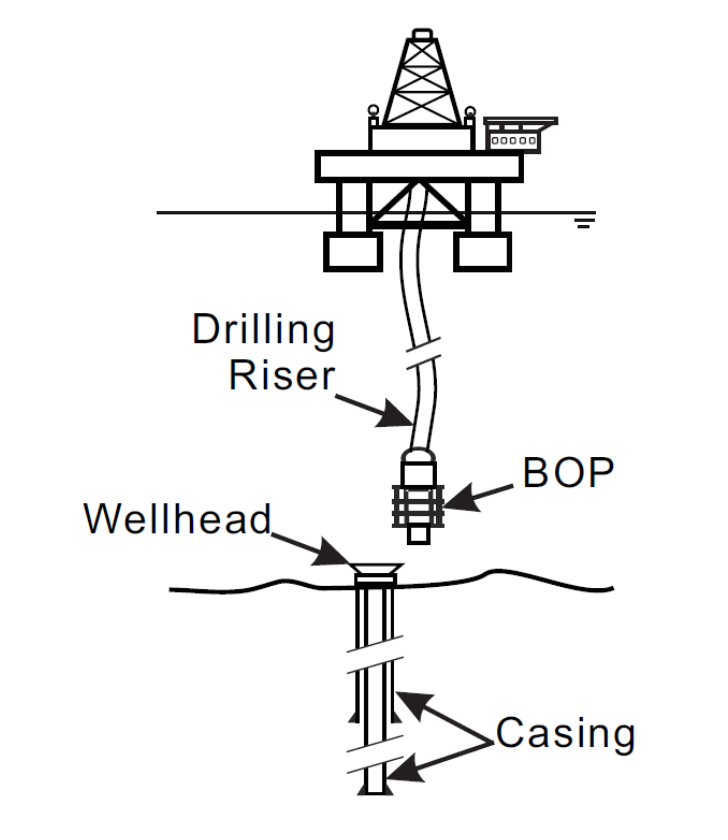
\includegraphics[width=5cm]{figs/introducao/riser}
  \caption{Operação de reentrada \cite{eugenioASME2012}\label{riser}}
\end{figure}


O foco deste trabalho está na operação de reentrada, conforme apresentada na Figura \ref{riser}. Atualmente, é uma operação feita manualmente por um operador na plataforma que observa remotamente as imagens capturas por \textit{ROV}s (\textit{Remotely Operated Vehicles}) da região do \textit{riser} próxima ao poço e controla a plataforma através de um \textit{joystick} com o auxílio do sistema de posicionamento dinâmico. O custo envolvido na operação é enorme e os riscos para o equipamento também, já que os próprios \textit{ROVs} e o \textit{riser} ficam sujeitos às perturbações das ondas, correntezas e variações ambientais no fundo do mar. A Figura \ref{posicionamentoAtual} apresenta o esquema que acabou de ser descrito.

\begin{figure}[hbt]
\centering
  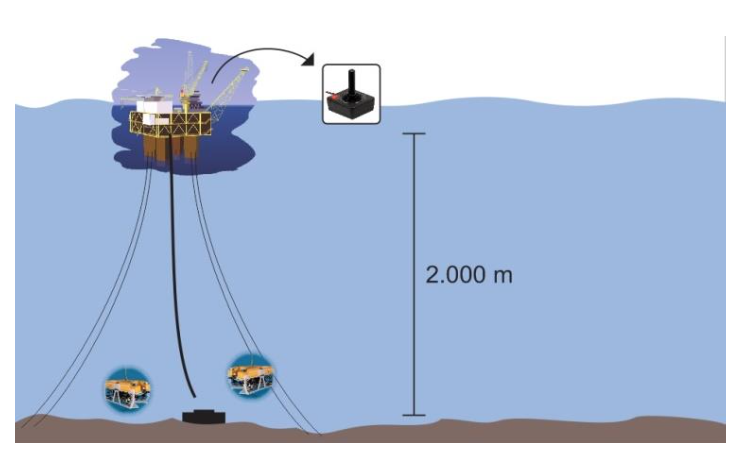
\includegraphics[width=8cm]{figs/introducao/posicionamentoAtual}
  \caption{Método atual para reconexão no poço \cite{redytton} \label{posicionamentoAtual}}
\end{figure}

O objetivo deste trabalho é apresentar uma forma mais eficiente de realizar a operação de reentrada, economizando tempo e recursos, evitando riscos para pessoal e equipamento. O trabalho de Rédytton \cite{redytton} validou 

\section{Definição do problema}

Definir problema.


\section{Objetivos do projeto}

Objetivos.


\section{Resultados obtidos}

Resultados.


\section{Apresentação do manuscrito}

Apresentar.


%Fundamentos
%TCIDATA{LaTeXparent=0,0,relatorio.tex}
\chapter{Fundamentos\label{chap:FundamentacaoMatematica}}

\resumodocapitulo{Este capítulo apresenta equações básicas do sistema que se deseja validar, assim como a redução modal utilizada, o projeto para obtenção dos ganhos para um dado conjunto de polos, e apresenta uma visão geral sobre o filtro de Kalman e o Preditor Smith. Também são expostas informações sobre a bancada laboratorial e sobre a programação do CLP.}

\section{Bancada\label{bancada}}
A bancada da ponte rolante presente no Laboratório de Automação e Controle está esquematizada na Figura \ref{bancadaEsquematico}. Serão detalhados os componentes desta bancada, de modo a se entender o papel de cada um deles. Observe que no esquemático falta a câmera, que é um sensor que fica de frente para a bancada. 

\begin{figure}[hbt]
\centering
  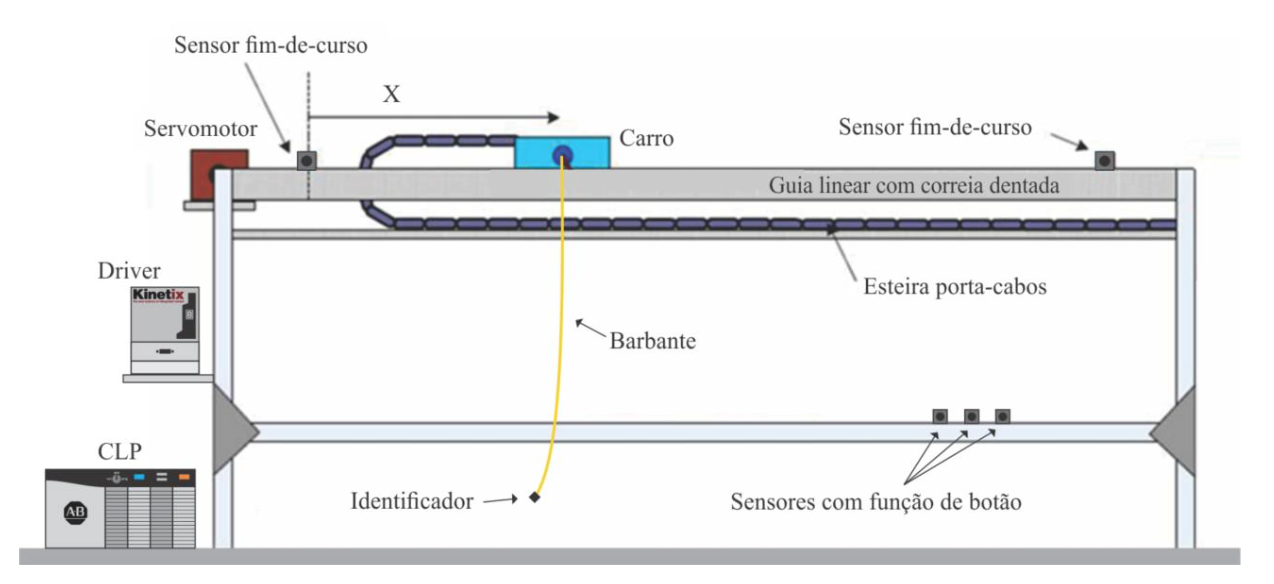
\includegraphics[width=0.8\textwidth]{figs/fundamentos/bancadaEsquematico}
  \caption{Esquemático da Bancada Utilizada para o Experimento \cite{redytton}\label{bancadaEsquematico}}
\end{figure}

\subsection{Controlador Lógico-Programável}
\begin{figure}[!ht]
  \centering
    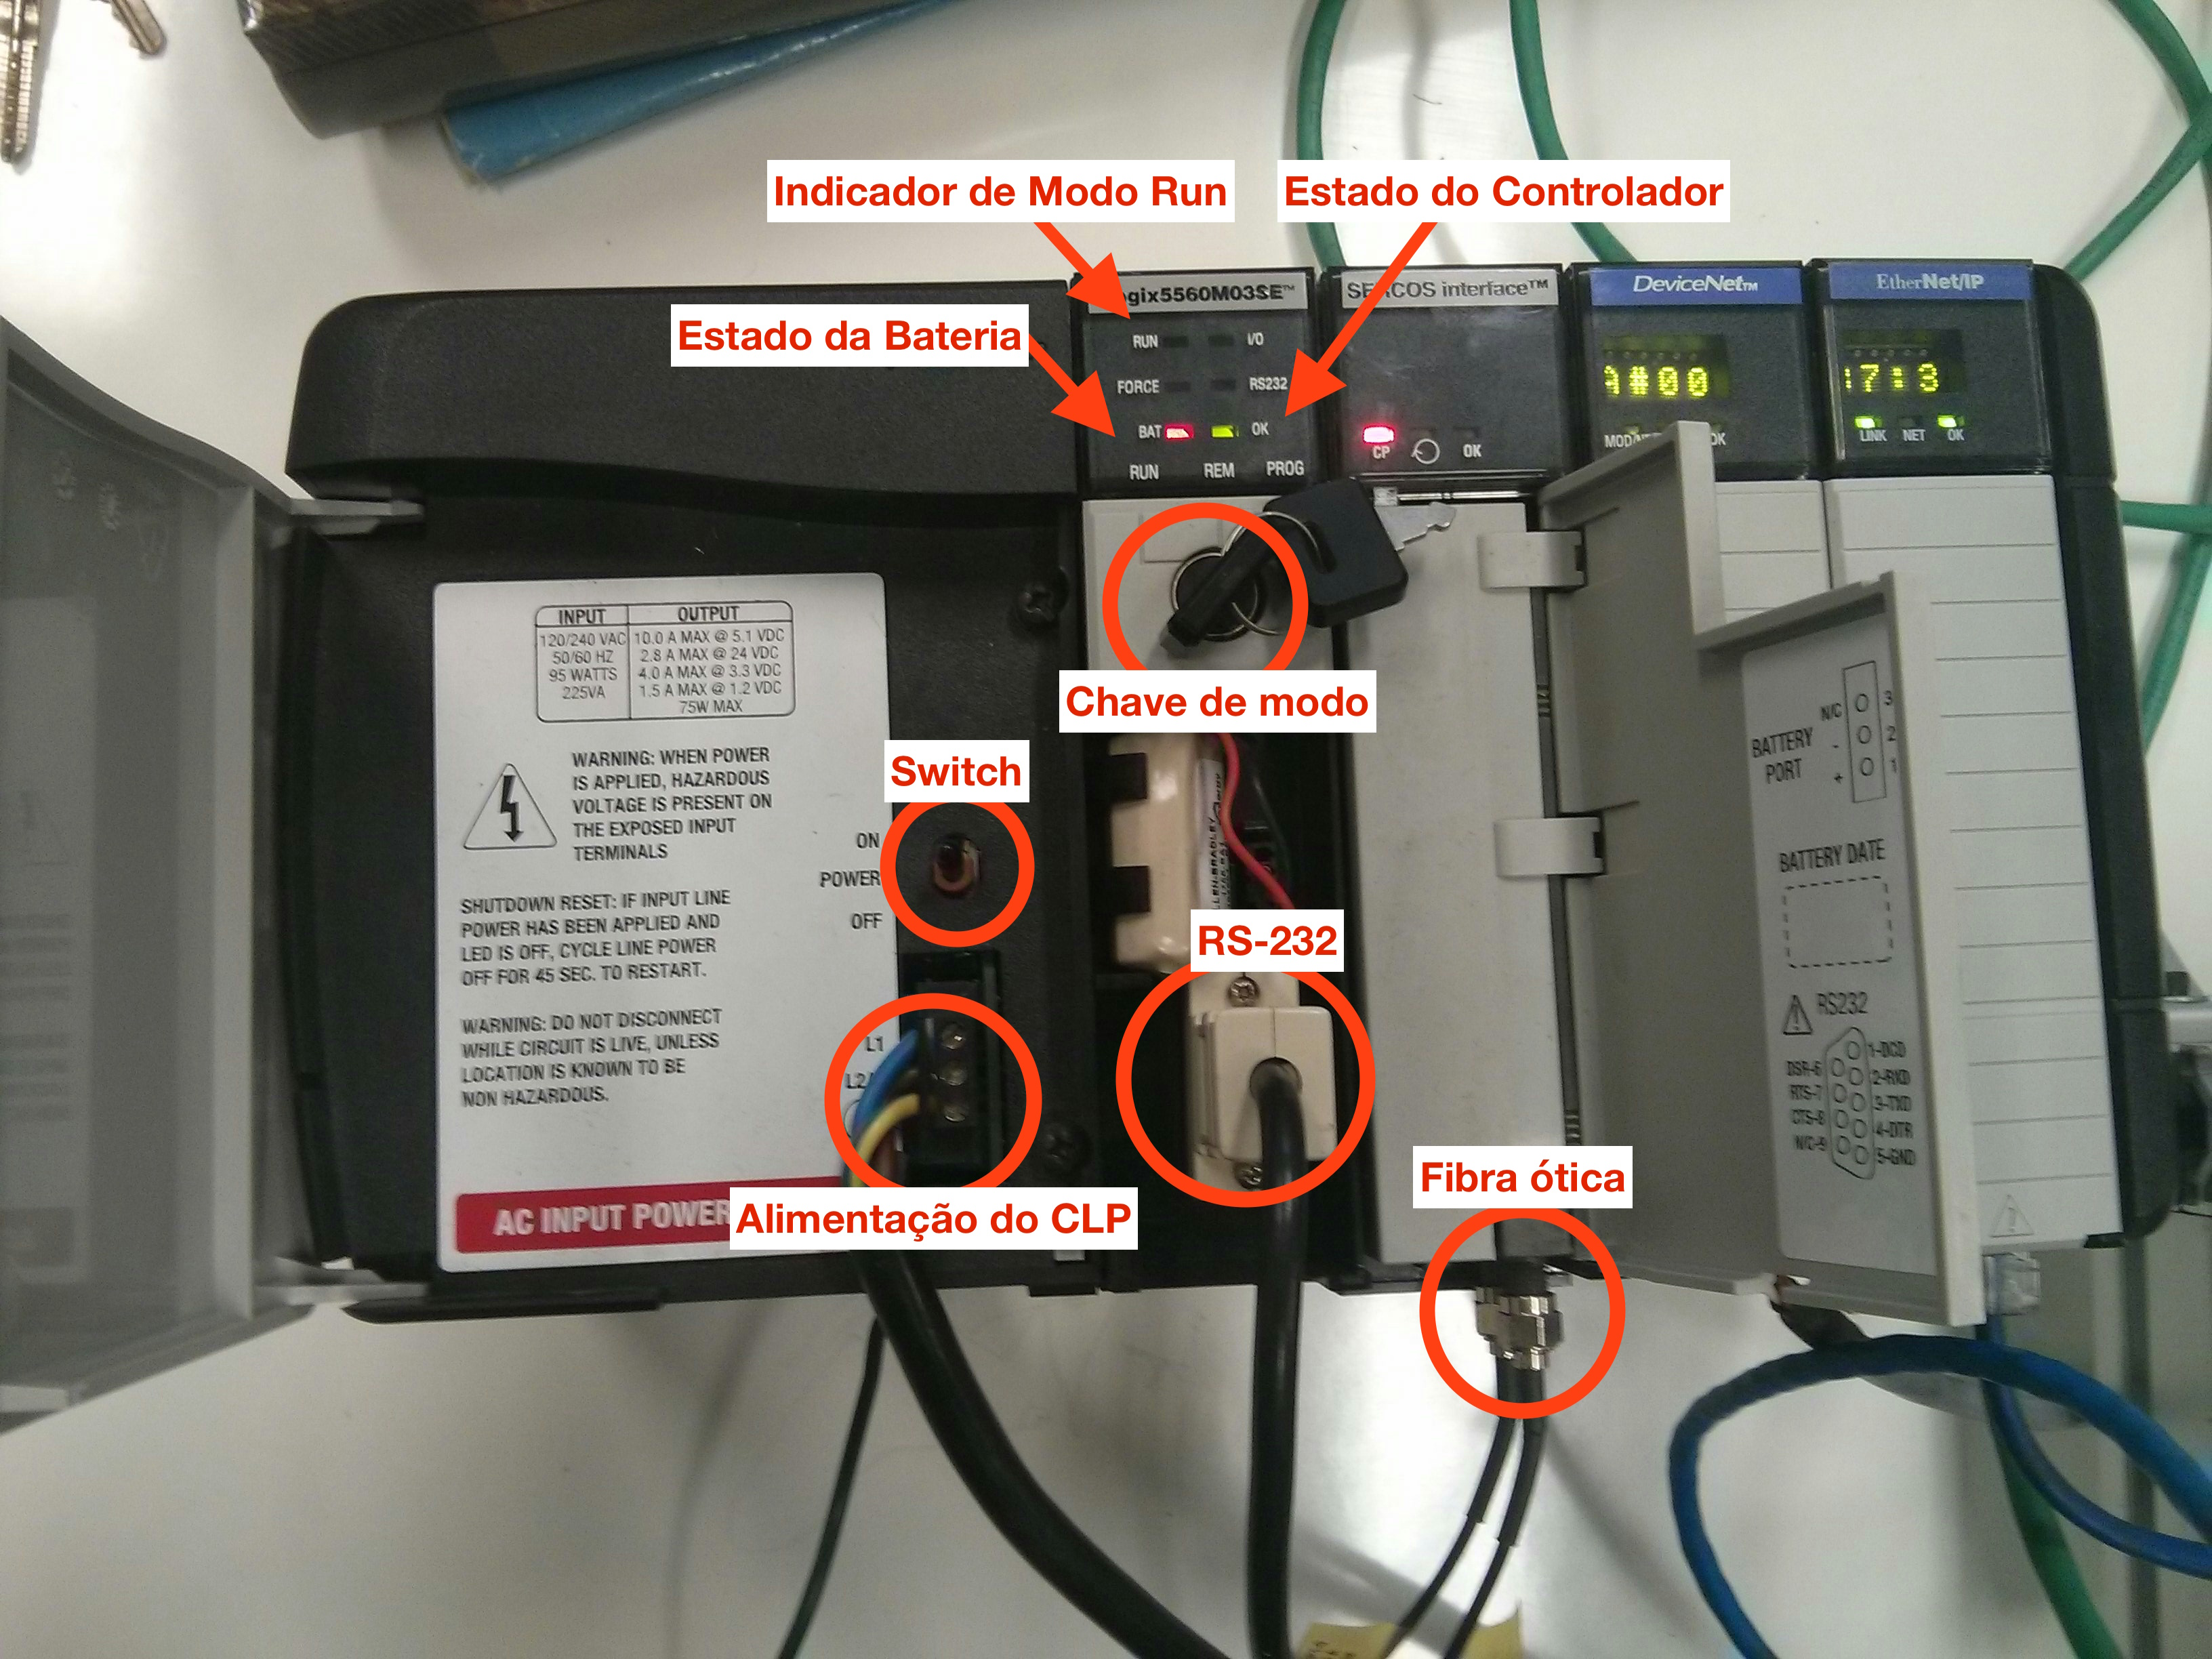
\includegraphics[width=0.8\textwidth]{figs/fundamentos/CLP.jpg}
    \caption{CLP com identificação de elementos\label{CLPcomentado}}
\end{figure}

O controlador lógico-programável (CLP - ver Figura \ref{CLPcomentado}) é a espinha dorsal da bancada. Ele é responsável por executar os comandos de controle sobre todos os elementos que estão conectados a ele. A programação do CLP é realizada pelo computador; porém, uma vez feito o \textit{download} do programa ao CLP, a execução ocorre independentemente do computador, contanto que o CLP esteja em modo de execução.

O CLP utilizado é fabricado pela \textit{Allen Bradley}, modelo Logix5560M03SE. Tal modelo possui memória lógica e de dados de 750 KiB, e memória de \textit{I/O} de 494 KiB. Há quatro módulos no \textit{chassis} do controlador:
\begin{itemize}
  \item O próprio controlador;
  \item \textit{SERCOS Interface};
  \item DeviceNET;
  \item EtherNet/IP.
\end{itemize}

Cada um desses módulos será apresentado posteriormente com mais detalhes. Além dos módulos, o controlador ainda possui um \textit{switch} liga/desliga presente no \textit{chassis}. No módulo Logix, há uma chave responsável por alterar o modo de funcionamento do mesmo. As posições possíveis dessa chave são:
\begin{itemize}
  \item RUN (\textit{Run mode});
  \item REM (\textit{Remote mode});
  \item PROG (\textit{Program mode});
\end{itemize}

Na prática, o modo REM se divide em dois modos: REM RUN e REM PROG. A maneira de se diferenciar os dois é observar, no módulo Logix, o estado do LED indicador de modo RUN quando a chave estiver na posição REM.

No modo RUN, o controlador apenas roda o programa presente em sua memória; não há qualquer comunicação remota. No modo PROG, o controlador não roda nenhum programa; ele apenas pode receber um novo código. Nos modos REM, há a comunicação com o computador, permitindo verificar valores de variáveis de interesse e alterar, se necessário, o programa a ser rodado pelo controlador. O programa presente no controlador, em modo REM, só roda o código se estiver no modo REM RUN; se for necessário atualizar o programa, o modo deve ser o REM PROG.

Para fins de se utilizar melhor o CLP, será utilizado sempre o modo REM e suas derivações. O modo REM RUM permite a execução do programa; já o modo REM PROG permite a atualização do programa dentro da memória do CLP.
\subsection{SERCOS Interface}

Sercos é um barramento digital de automação que interconecta controladores, \textit{drives}, dispositivos de entrada/saída e atuadores para máquinas e sistemas controlados numericamente. Foi projetado para comunicação serial de alta velocidade de dados em sistemas de tempo real por meio de fibra ótica (Sercos I \& II) ou um cabo Ethernet Industrial (Sercos III). Sercos é um padrão internacional \cite{sercos}.

Num sistema Sercos, todas as malhas que contém servomotores são normalmente fechadas no \textit{drive}. Isto reduz a carga computacional no CLP, permitindo-o sincronizar mais eixos do que conseguiria caso contrário. Além disso, fechar a malha dos servomotores com o \textit{driver} ajuda a reduzir o efeito do atraso de transporte entre o controle de movimento e o \textit{driver} \cite{sercos}.

Nesta bancada, o CLP deve se comunicar com o servomotor (MPL-A310F-SJ22AA) através do \textit{drive} Kinetix (2094-AC05MP5), de forma a movimentar o carrinho segundo uma trajetória planejada ou segundo uma lei de controle em malha fechada executando no CLP. Essa comunicação se dá por um par de fibras óticas full-duplex, conforme se observa na Figura \ref{CLPcomentado}, o que caracteriza uma rede Sercos I ou II.

\subsection{Line Interface Module 2094-AL09}

Este módulo não apareceu no esquemático da Figura \ref{bancadaEsquematico}, mas ele tem a função essencial de interfacear a rede trifásica com o servo \textit{drive}, permitindo o acionamento do motor. Na Figura \ref{LineInterfaceModule}, se observa que há três conjuntos de disjuntores nesse módulo: CB1 \textendash{} liga ou desliga a rede trifásica do \textit{drive}  \textendash{}, CB2 \textendash{} fornece tensão monofásica ao servo \textit{drive} \textendash{} e CB3 \textendash{} liga as duas fontes de tensão DC de 24V \textendash{}, responsáveis pelas entradas e saídas digitais do módulo e alimentação do freio do motor \cite{redytton}.

\begin{figure}[!ht]
  \centering
    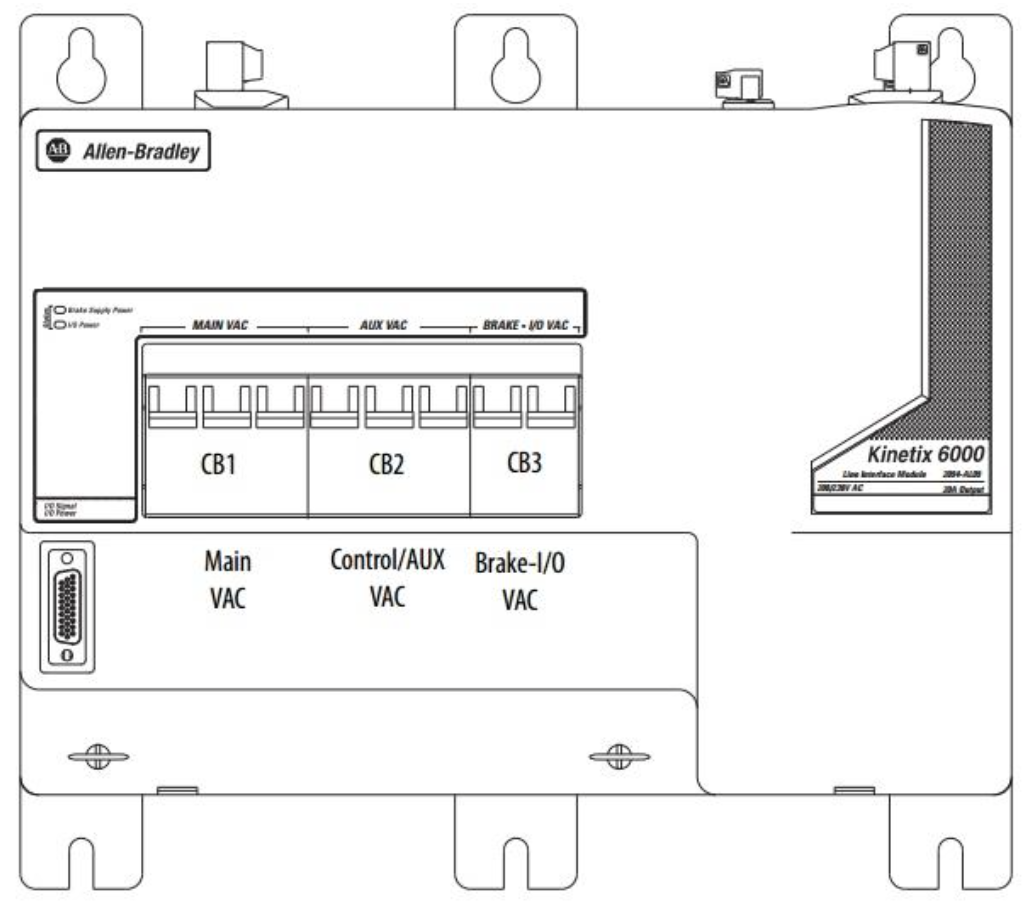
\includegraphics[width=0.7\textwidth]{figs/fundamentos/LineInterfaceModule}
    \caption{Line Interface Module modelo 2094-AL09 da Allen Bradley \cite{redytton}\label{LineInterfaceModule}}
\end{figure}

\subsection{Drive Kinetix 6000 da Allen Bradley}

Por meio da Interface Sercos, o CLP comanda o drive que então fornece potência ao motor. O drive controla o servomotor por meio de pulsos PWM. A Figura \ref{kinetix6000} apresenta um Drive Kinetix 6000 da Allen Bradley similar ao utilizado no laboratório. Mais detalhes sobre o funcionamento do drive estão disponíveis em \cite{redytton} e \cite{kinetix6000usermanual}.

\begin{figure}[!ht]
  \centering
    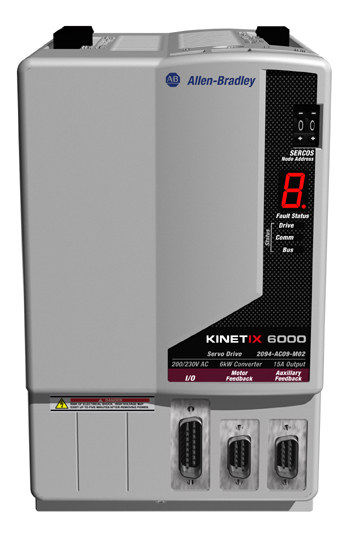
\includegraphics[width=0.3\textwidth]{figs/fundamentos/kinetix6000.jpg}
    \caption{Drive Kinetix 6000 da Allen Bradley\label{kinetix6000}}
\end{figure}

\subsection{Servomotor}

Um servomotor é um atuador rotatório que permite controle preciso da posição angular. O motor consiste de um motor acoplado a um sensor para a realimentação de posição/velocidade. Também é necessário um drive servo para completar o sistema. O \textit{drive} usa o sensor de realimentação para controlar precisamente a posição angular do motor, ou seja, é uma operação em malha fechada. Assim, usando servomotores em malha fechada, tem-se uma alternativa de alto desempenho aos motores de passo e de indução \cite{defServoMotores}.

O servomotor MPL-A310F-SJ22AA da \textit{Allen-Bradley} foi utilizado e está representado na Figura \ref{servomotor}. O mesmo é composto por um motor indutivo de tensão nominal $230V_{\mathrm{ac}}$ e um encoder do tipo StegmanHiperface, que mede posição de forma absoluta e velocidade de forma incremental \cite{redytton}.

\begin{figure}[!ht]
  \centering
    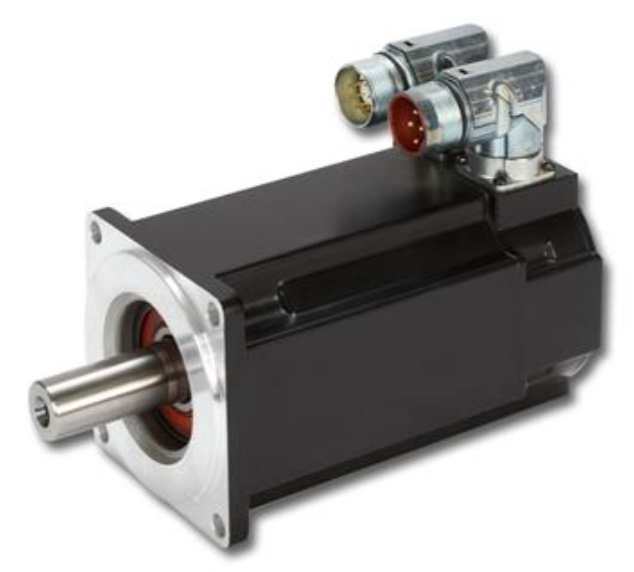
\includegraphics[width=0.3\textwidth]{figs/fundamentos/servomotor}
    \caption{Servomotor modelo MPL-A310F-SJ22AA\label{servomotor}}
\end{figure}

\subsection{Sensores indutivos}
Os sensores indutivos são elementos detectores de presença, particularmente de objetos metálicos. Eles funcionam através da variação de campo magnético ocasionada pela presença do objeto a ser identificado. Tal variação de campo magnético provoca uma variação de corrente dentro do sensor, alterando seu estado.

Na presente bancada, há 6 sensores indutivos da família 871TM, similares ao da Figura \ref{sensorIndutivo}, fabricados pela \textit{Allen-Bradley}. Eles são alimentados com tensão de 24 V, que está dentro dos limites padrão. São sensores feitos de aço, adaptados a ambientes industriais.

\begin{figure}[!ht]
  \centering
    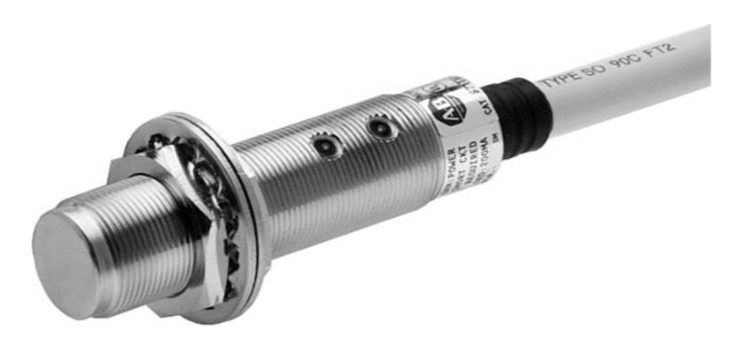
\includegraphics[width=0.3\textwidth]{figs/fundamentos/sensorIndutivo}
    \caption{Sensor indutivo 871T-R8B18 \cite{redytton}\label{sensorIndutivo}}
\end{figure}

A importância desses sensores é enorme. O motivo é que a câmera às vezes falha para obter a posição atual e tem um limite de frequência devido ao processamento interno que ela tem de realizar. Com os sensores indutivos, tem-se um processamento rápido para identificar se o motor está na região próxima dos limites. Assim, a rotina de segurança que trava o motor depende diretamente desses sensores indutivos, como mostra o Anexo \ref{emergencyladder}.

\subsection{Câmera PresencePlus}

A câmera PresencePlus P4 GEO da Banner Engineering foi utilizada no projeto - veja Figura \ref{cameraBanner}. Esta câmera é um sensor robusto utilizado em ambientes industriais com fácil utilização. Sua programação é feita em software próprio da Banner e é visual.

Dentre as capacidades da câmera, nota-se que ela pode capturar até 24 imagens por segundo. No entanto, além da captura das imagens há o processamento das imagens, que pode ser feito na própria câmera ou em um módulo externo da própria Banner, que também consome certo tempo. O programa utilizado no projeto está disponível no Anexo \ref{ballhorzpos}.

\begin{figure}[!ht]
  \centering
    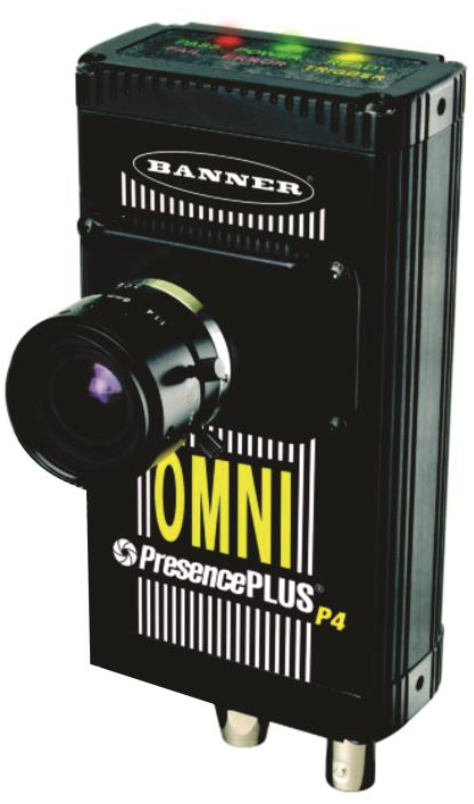
\includegraphics[width=0.3\textwidth]{figs/fundamentos/camera}
    \caption{Câmera da Banner Engineering utilizada no projeto \cite{redytton}\label{cameraBanner}}
\end{figure}

\section{Modelagem\label{modelagem}}
\subsection{Equações Governantes}

Estruturas submarinas tais como os \textit{risers} são esbeltas e tem um alto módulo de cisalhamento. Portanto, a simplificação de Euler-Bernoulli para vigas é utilizada para propósitos de modelagem. O deslocamento de interesse é o horizontal e o \textit{riser} está sob a ação de forças hidrodinâmicas externas e de tração. A equação diferencial parcial para a variável deslocamento, $\Upsilon$, é dada por \begin{align}
	m_s \frac{\partial^2 \Upsilon}{\partial t^2} &= -E J	\frac{\partial^4 \Upsilon}{\partial z^4} + \frac{\partial}{\partial z}\left(T(z) \frac{\partial \Upsilon}{\partial z}\right) + F_n(z,t)\label{equacaoMorison},
\end{align} na qual $m_s$ é a densidade linear do tubo, $E$ é o módulo de Young e $J$ é o segundo momento de inércia do \textit{riser}. $T(z)$ descreve as forças de tração ao longo do comprimento do \textit{riser}. $F_n(z,t)$ é a força resultante externa --- força linear, unidade N/m \cite{fabricioIFAC}. 

No caso do problema em escala laboratorial que foi trabalhado, o tubo é representado por um barbante e daqui em diante serão discutidas e apresentadas as variáveis necessárias para se trabalhar com esse problema: \begin{itemize}
	\item $m_s$ é a massa linear do barbante (densidade linear, kg/m);
	\item $E$ é o módulo de Young do barbante e ele é desconhecido;
	\item $J$ é o segundo momento de área e representa a resistência do barbante à flexão -- como o barbante não apresenta tal resistência, $J=0$;
	\item $T(z)$ é a força de tração e é dada por \[T(z) = \left(m_b+z m_s\right)g,\] sendo $m_b$ a massa da bolinha (kg), $m_s = m_{\textrm{barbante,kg}}/L$, sendo $L$ o comprimento do barbante, $z$ a posição vertical a partir do carrinho e $g$ é a força da gravidade.
\end{itemize}


As únicas forças externas atuando no \textit{riser} são hidrodinâmicas, exceto nas extremidades do topo e do fundo, nas quais forças de reação seguem condições de contorno. A equação de Morison descreve a força externa resultante, dada por \begin{align}
	F_n(z,t) &= -m_{fbar} \frac{\partial^2 \Upsilon}{\partial t^2} - \mu \left|\frac{\partial \Upsilon}{\partial t}\right|\frac{\partial \Upsilon}{\partial t}\label{forceN},
\end{align} na qual $\mu$ é o coeficiente de arrasto (unidade 1/s) e $m_{fbar}$ é a massa do fluido adicionado, que será posteriormente pormenorizada. Fazendo $m = m_s + m_{fbar}$ e substituindo a Equação \ref{forceN} na \ref{equacaoMorison}, obtém-se \begin{align}
	\frac{\partial^2 \Upsilon}{\partial t^2} &= -\frac{EJ}{m}\frac{\partial^4 \Upsilon}{\partial z^4} + \frac{\partial}{\partial z}\left(\frac{T(z)}{m}\frac{\partial \Upsilon}{\partial z}\right) - \frac{\mu}{m}\left|\frac{\partial \Upsilon}{\partial t}\right|\frac{\partial \Upsilon}{\partial t}.
\end{align}

Em relação à massa do fluido adicionado, $m_{fbar}$ é dada por \begin{align}
	m_{fbar} &=  2 \pi r_{bar}^2 \rho_{\mathrm{ar}}\nonumber\\
	&= 0.00770\;\mathrm{g/m}.
\end{align} 

 Já que $m_{fbar} \ll m_s$ conforme a Tabela \ref{constanteBarbante}, consideraremos $m \approx m_s$ nos cálculos. Em relação à massa $m_{fb}$ do fluido adicionado ao redor da bolinha de isopor, ela é dada por\begin{align}
	m_{fb} &= 1.2 V_{b} \rho_{\mathrm{ar}}\nonumber\\
	&= 1.2 \left(\frac{4}{3}\pi r_b^3\right)\rho_{\mathrm{ar}}\nonumber\\
	&= 0.0220\;\textrm{g},
\end{align} de onde se pode observar que $m_{fb} \ll m_{b}$, conforme Tabela \ref{constanteIsopor}. Assim,  os cálculos consideraram $m' \approx m_b$.

\begin{table}[!ht]
	\centering
	\caption{Constantes do barbante\label{constanteBarbante}}
	\begin{tabular}{|l|c|c|c|}
		\hline
		\textbf{Significado} & \textbf{Símbolo} & \textbf{Valor} & \textbf{Unidade}\\ \hline \hline
		Massa & $m_{bar}$ & 0.492 & g\\ \hline
		Comprimento & $L$ & 0.82 & m \\ \hline
		Massa linear & $m_s$ & 0.6 & g/m\\ \hline
		Raio & $r_{bar}$ & 1 & mm\\ \hline
		Densidade & $\rho_{bar}$ & 191 & kg/m$^3$\\ \hline
	\end{tabular}
	
\end{table}

\begin{table}[!ht]
	\centering
	\caption{Constantes da bolinha de isopor\label{constanteIsopor}}
	\begin{tabular}{|l|c|c|c|}
		\hline
		\textbf{Significado} & \textbf{Símbolo} & \textbf{Valor} & \textbf{Unidade}\\ \hline \hline
		Massa & $m_{b}$ & 0.492 & g\\ \hline
		Raio & $r_{b}$ & 15.3 & mm\\ \hline
		Coeficiente de inércia & $C_m$ & 1.2 & - \\ \hline
		Coeficiente de arrasto & $C_d$ & 0.6 & - \\ \hline
		Volume & $V_b$ & $\frac{4}{3}\pi r_b^3$ & $\textrm{m}^3$ \\ \hline
		Área da seção transversal & $A_b$ & $\pi r_b^2$ & m$^2$\\ \hline
	\end{tabular}
	
\end{table}

 Um ponto importante de se notar é que o barbante pesa mais do que o isopor, o que faz com que a tração não seja principalmente devida pela bolinha, mas sim pelo barbante. Neste caso, não se utiliza um valor médio para $T(z)$ como em \cite{fabricioIFAC}, mas ainda se pode usar um valor médio para as constantes $\tau$ e $\tau'$, que substituem o termo $\frac{\mu}{m}\left|\frac{\partial \Upsilon}{\partial t}\right|$ para o barbante e para a bolinha, respectivamente. Essas constantes são definidas de acordo com a trajetória prevista, uma vez que a velocidade média depende dessa trajetória. Já levando em conta um valor médio para $\left|\frac{\partial \Upsilon}{\partial t}\right|$, tem-se \begin{align}
	\frac{\partial^2 \Upsilon}{\partial t^2} &= -\frac{EJ}{m}\frac{\partial^4 \Upsilon}{\partial z^4} + \frac{\partial}{\partial z}\left(\frac{T(z)}{m}\frac{\partial \Upsilon}{\partial z}\right) - \tau\frac{\partial \Upsilon}{\partial t}.\label{EquacaoComTau}
	\end{align}

 Neste trabalho, fizeram-se experimentos com uma excursão do carrinho de 30cm. O valor de $\tau$ e $\tau'$ foi calculado por Rafael Simões \cite{rafaelMestrado}. Para o barbante, $\tau = 0.2426/\mathrm{s}$. Para a bolinha, $\tau'=0.1133/\mathrm{s}$.
 
 Antes de se prosseguir para a discretização e obtenção das matrizes em espaço de estados, é importante pensar nas condições de contorno. No topo, $z=L$, tem-se $\Upsilon(L,t)=u(t)$, ou seja, o carrinho se move conforme uma trajetória $u(t)$ definida. Neste mesmo ponto, $\frac{\partial\Upsilon}{\partial z}(L,t) = 0$. Para a ponta na qual a carga está situada, $z=0$, tem-se $\frac{\partial\Upsilon}{\partial z}(0,t) = \frac{F_L}{T}$, sendo $F_L$ a força aplicada pela ponta do riser na carga.

\subsection{Discretização}
O objetivo desta seção é representar a Equação \ref{EquacaoComTau} em um espaço de estados finito discreto.  Para isso, aplica-se o método de diferenças finitas na coordenada $z$ de maneira a se aproximar a EDP governante em um número finito de EDOs \cite{fabricioIFAC}. No espaço discreto, a equação do $k$-ésimo elemento é dada por \begin{align}
	\frac{d^2\Upsilon_k}{dt^2} &= -\frac{EJ}{m l^4}\left(\Upsilon_{k-2} - 4\Upsilon_{k-1}+6\Upsilon_{k}-4\Upsilon_{k+1}+\Upsilon_{k+2}\right)\nonumber\\
	&+ \frac{T_0+mg(k-1)l}{m l^2}\left(\Upsilon_{k-1}-2\Upsilon_{k} + \Upsilon_{k+1}\right)+g\frac{-\Upsilon_{k-1}+\Upsilon_{k+1}}{2l}-\tau\frac{d\Upsilon_k}{dt},
\end{align} sendo $N$ o número de pontos de discretização e $l$ a distância entre dois pontos vizinhos ($l = L/N$).

 Deve-se notar que $k\in \mathbb{N}:2\le k \le N-1$, pois um dos extremos é a bolinha, caso no qual $k=1$, e a equação do pêndulo rege seu movimento, enquanto que na outra ponta, $k=N$, se aplica uma condição de contorno que é a entrada da planta $u(t)$. O que aconteceria quando $k=2$ e se precisasse de $\Upsilon_{k-2}$? Para o presente experimento, $J=0$ e esse problema não ocorre. Caso se façam testes com um valor de $J\neq 0$, é necessário resolver esse problema primeiro. Uma solução seria utilizar diferenças finitas unilaterais para esses pontos próximos à fronteira.

 Para simplificar, definem-se as constantes \begin{align}
	a &= -\frac{EJ}{m l^4},\\
	b_k &= \frac{T_0 + mg(k-1)l}{m l^2},\; k\ge 2,\\
	c &= \frac{g}{2l},\\
	d_k &= b_k - c,\; k\ge 2\;\mathrm{e}\\
	e_k &= b_k + c,\; k\ge 2.
\end{align}

 Uma estratégia para se analisar como as matrizes do espaço de estados do sistema ficarão é escolher um número de pontos $N$ pequeno e escrever todas as equações. Depois de compreendido o padrão desse sistema pequeno, pode-se generalizar e criar uma rotina que crie as matrizes para qualquer $N$. Observa-se que $a=0$ para o barbante, pois $J=0$, como apresentado anteriormente, o que simplifica os cálculos.

 Para o caso $N=6$, por exemplo, tem-se \begin{align}
\mathbf{x} &= \left(\Upsilon_1\;\Upsilon_2\;\Upsilon_3\;\Upsilon_4\;\Upsilon_5\;\Upsilon_6\;\dot{\Upsilon}_1\;\dot{\Upsilon}_2\;\dot{\Upsilon}_3\;\dot{\Upsilon}_4\;\dot{\Upsilon}_5\;\dot{\Upsilon}_6\right)^T, 	\\
u &= \Upsilon(L,t) = \Upsilon_7\label{ufor6}\;\mathrm{e}\\
y &= \Upsilon(0,t) = \Upsilon_1\label{yfor6}.
 \end{align} 
 
 Para o vetor $\mathbf{\dot{x}}$ de interesse, as equações para os estados de velocidade $\dot{\Upsilon}_i$, $1 \le i \le 6$, já fazem parte do vetor de estados, então não é necessário discriminá-las. Já para os pontos de aceleração fora o da bolinha $\ddot{\Upsilon}_i$, $2 \le i \le 6$, suas equações são dadas por \begin{align}
 	\ddot{\Upsilon}_2 &=  b_2\left(\Upsilon_{1}-2\Upsilon_{2} + \Upsilon_{3}\right)+c(-\Upsilon_1 + \Upsilon_3)-\tau \dot{\Upsilon}_2\nonumber \\
 	&= d_2\Upsilon_1 - 2b_2 \Upsilon_2 + e_2\Upsilon_3 - \tau \dot{\Upsilon}_2, \label{upsilon2}\\
 	\ddot{\Upsilon}_3 &=  b_3\left(\Upsilon_{2}-2\Upsilon_{3} + \Upsilon_{4}\right)+c(-\Upsilon_2 + \Upsilon_4)-\tau \dot{\Upsilon}_3\nonumber \\
 	&= d_3\Upsilon_2 - 2b_3 \Upsilon_3 + e_3\Upsilon_4 - \tau \dot{\Upsilon}_3,\\
 	\ddot{\Upsilon}_4 &=  b_4\left(\Upsilon_{3}-2\Upsilon_{4} + \Upsilon_{5}\right)+c(-\Upsilon_3 + \Upsilon_5)-\tau \dot{\Upsilon}_4, \nonumber\\
 	&= d_4\Upsilon_3 - 2b_4 \Upsilon_4 + e_4\Upsilon_5 - \tau \dot{\Upsilon}_4,\\
 	\ddot{\Upsilon}_5 &=  b_5\left(\Upsilon_{4}-2\Upsilon_{5} + \Upsilon_{6}\right)+c(-\Upsilon_4 + \Upsilon_6)-\tau \dot{\Upsilon}_5\nonumber\\
 	&= d_5\Upsilon_4 - 2b_5 \Upsilon_5 + e_5\Upsilon_6 - \tau \dot{\Upsilon}_5\;\mathrm{e}\\
 	\ddot{\Upsilon}_6 &=  b_6\left(\Upsilon_{5}-2\Upsilon_{6} + u\right)+c(-\Upsilon_5 + u)-\tau \dot{\Upsilon}_6\nonumber\\
 	&= d_6\Upsilon_5 - 2b_6 \Upsilon_6 + e_6 u - \tau \dot{\Upsilon}_6. \label{upsilon6}
 \end{align}

 A equação para a posição da carga $\Upsilon_1$ leva em conta a massa da bolinha e a força de Morison e é dada por \begin{align}
 	m_b \ddot{\Upsilon}_1 &= \frac{m_b g}{l}\left(\Upsilon_2 - \Upsilon_1\right) + \rho_{\mathrm{ar}} C_m V_b \ddot{\Upsilon}_1 - \frac{1}{2}\rho_{\textrm{ar}} C_d A_b \dot{\Upsilon}_1 \left|\dot{\Upsilon}_1\right|.\label{upsilon1previa}
 \end{align} 
 
 Isolando $\ddot{\Upsilon}_1$ na Equação \ref{upsilon1previa}, tem-se \begin{align}
 	\ddot{\Upsilon}_1 &= \frac{m_b g}{m'l}\left(\Upsilon_2 - \Upsilon_1\right)  - \frac{1}{2m'}\rho C_d A_b \dot{\Upsilon}_1 \left|\dot{\Upsilon}_1\right|.
 \end{align} 
 
  Nota-se que $m' = m_b + \rho_{\textrm{ar}} C_m V_b = m_b + m_{fb} \approx m_b$. Assim, assume-se $m' = m_b$ para os cálculos. Anteriormente, foi apresentada a linearização $\tau$ para o termo $\frac{1}{2m}\rho C_d A\left|\dot{\Upsilon}_k\right|$ do cabo. Para o caso da bolinha de isopor, essa constante é diferente e é denotada por $\tau'$, resultando na equação final para $\Upsilon_1$, que é \begin{align}
 	\ddot{\Upsilon}_1 &= b_1\left(-\Upsilon_1 + \Upsilon_2\right) - \tau'\dot{\Upsilon}_1\label{upsilon1final},
 \end{align} sendo \begin{equation}
 	b_1 = \frac{m_b g}{m'l} = \frac{g}{l}.
 \end{equation}

  Desta forma, a partir das Equações \ref{upsilon1final} e \ref{upsilon2}-\ref{upsilon6}, pode-se definir o sistema linear em forma matricial, resultando em \begin{align}
 	\mathbf{\dot{x}} &= \left[\begin{array}{cccccccccccc}
 		0 & 0 & 0 & 0 & 0 & 0 & 1 & 0 & 0 & 0 & 0 & 0\\
 		0 & 0 & 0 & 0 & 0 & 0 & 0 & 1 & 0 & 0 & 0 & 0\\
 		0 & 0 & 0 & 0 & 0 & 0 & 0 & 0 & 1 & 0 & 0 & 0\\
 		0 & 0 & 0 & 0 & 0 & 0 & 0 & 0 & 0 & 1 & 0 & 0\\
 		0 & 0 & 0 & 0 & 0 & 0 & 0 & 0 & 0 & 0 & 1 & 0\\
 		0 & 0 & 0 & 0 & 0 & 0 & 0 & 0 & 0 & 0 & 0 & 1\\
 		-b_1 & b_1 & 0 & 0 & 0 & 0 & -\tau' & 0     & 0 & 0 & 0 & 0\\
 		d_2 & -2b_2  & e_2  & 0  & 0 & 0 &  0    & -\tau & 0 & 0 & 0 & 0\\
 		0 & d_3 & -2b_3  & e_3  & 0  & 0 & 0 &  0    & -\tau & 0 & 0 & 0\\
 		0 & 0 & d_4 & -2b_4  & e_4  & 0  & 0 & 0 &  0    & -\tau & 0 & 0\\
 		0 & 0 & 0 & d_5 & -2b_5  & e_5  & 0  & 0 & 0 &  0    & -\tau & 0\\
 		0 & 0 & 0 & 0 & d_6 & -2b_6  & 0  & 0 & 0 &  0    & 0   &-\tau\\
 	\end{array}\right]\mathbf{x} + \left[\begin{array}{c}
	0\\	0\\	0\\	0\\	0\\ 0\\ 0\\ 0\\ 0\\ 0\\ 0\\ e_6
\end{array}
\right]u,
 \end{align} que pode ser representado concisamente como \begin{align}
 	\mathbf{\dot{x}} &= \left[\begin{array}{cc}
	\mathbf{0}_{6\times 6} & \mathbf{I}_{6\times 6}\\
	\mathbf{M}_{6\times 6} & \mathbf{L}_{6\times 6}\\
\end{array}\right] \mathbf{x} + \left[\begin{array}{c}
	\mathbf{0}_{11\times 1}\\ e_6\\
\end{array} \right]u.
 \end{align}

 Para o caso de uma discretização com $N$ pontos, tem-se \begin{align}
 	\mathbf{\dot{x}} &= \left[\begin{array}{cc}
	\mathbf{0}_{N\times N} & \mathbf{I}_{N\times N}\\
	\mathbf{M}_{N\times N} & \mathbf{L}_{N\times N}\\
\end{array}\right] \mathbf{x} + \left[\begin{array}{c}
	\mathbf{0}_{2N-1\times 1}\\ e_N\\
\end{array} \right]u,\;\;\\
y &= \left[\begin{array}{cc}
	1 & \textbf{0}_{1\times 2N-1}
\end{array}\right]\textbf{x}.
 \end{align}


\subsection{Estratégia de Redução da ordem do modelo\label{reducaoModal}}

 A maior parte da teoria clássica de controle lida com sistemas representados por um pequeno número de variáveis de estado. Portanto, uma forma de aplicar métodos clássicos de controle da literatura para sistemas de parâmetros distribuídos discretos é por meio de uma redução da ordem do modelo \cite{fabricioIFAC}.

 Tal redução do modelo será feita em duas etapas: primeiro, uma transformação modal é aplicada nas equações originais do espaço de estados, resultando em uma nova representação em variáveis modais. Nesta forma, o sistema pode ser visto como um conjunto de subsistemas dissociados em paralelo, cuja influência na saída pode ser calculada individualmente. Então, os subsistemas com os maiores ganhos estáticos são escolhidos para criar um modelo de ordem reduzida \cite{fabricioIFAC}.

 Primeiro, deve-se obter os autovalores do espaço de estados do \textit{riser}. Observa-se que eles são sempre distintos entre si, uma condição suficiente para a diagonalização da matriz do espaço de estados. Assim, calcula-se a matriz modal \textbf{T}, cuja i-ésima coluna é o i-ésimo autovetor do sistema: \begin{align}
	\mathbf{T} &= \left(\;\mathbf{v_1}\;|\;\mathbf{v_2}\;|\;\ldots\;|\;\mathbf{v_{2N}}\;\right)_{1\times 2N}
\end{align}

 A matriz $\mathbf{T}$ provavelmente tem valores complexos. Isso é um problema para a representação em espaço de estados e sua simulação. A solução é criar uma matriz $\mathbf{\tilde{T}}$ que tenha só números reais. Antes de explicar como criá-la, deve-se lembrar que que os autovalores complexos sempre aparecem em pares conjugados, já que a matriz $\mathbf{A}$ só tem valores reais. Quando a primeira coluna de um autovetor de um par complexo conjugado for encontrada, a coluna respectiva de $\mathbf{\tilde{T}}$ será sua parte real. A segunda coluna desse par complexo conjugado será a parte imaginária da coluna de $\mathbf{T}$.


 A matriz $\mathbf{\tilde{T}}$ é utilizada para uma transformação de similaridade no sistema original: \begin{align}
	\mathbf{A_M} &= \mathbf{\tilde{T}}^{-1}\mathbf{A}\mathbf{\tilde{T}},\\
	\mathbf{x_M} &=\mathbf{\tilde{T}}^{-1}\mathbf{x},	\\
	\mathbf{B_M} &= \mathbf{\tilde{T}}^{-1}\mathbf{B},\textrm{ e}\\
	\mathbf{C_M} &=\mathbf{C}\mathbf{\tilde{T}}.
\end{align}


 O sistema transformado, denotado pelo subscrito $\mathbf{M}$, é mais adequado à análise. $\mathbf{A_M}$ é uma matriz diagonal por blocos, com seus autovalores explícitos, e permitindo o desacoplamento do sistema original em $N$ subsistemas formados por pares de autovalores reais ou complexo-conjugados. Nota-se que cada subsistema é de ordem 1 ou 2 dependendo se o autovalor é real ou um par complexo conjugado.

 Neste estágio, procura-se determinar quais dos subsistemas são mais adequados para aproximar o modelo original por meio do cálculo do ganho estático de cada um. Este método depende da predominância de uns poucos autovalores na resposta do sistema, já que altas frequências são muito atenuadas pelas forças hidrodinâmicas e pela suavidade da entrada.

 Os subsistemas selecionados são combinados em um modelo reduzido dado por \begin{align}
	\mathbf{\dot{z}} &= \mathbf{A_R}\mathbf{z}+\mathbf{B_R}u\;\mathrm{e}\\
	y &= \mathbf{C_R}\mathbf{z}+\mathbf{D_R}u,
\end{align} cuja ordem é escolhida considerando o custo-benefício entre a acurácia da dinâmica reduzida e a simplicidade da estrutura de controle exigida. Além disso, o sistema reduzido deve compensar o ganho estático perdido nos autovalores desconsiderados. Isto é feito por meio de uma matriz de transferência direta $\mathbf{D_R}$, que é a diferença dos ganhos dos sistemas original e reduzido: \begin{align}
	\mathbf{D_R}&=\mathbf{C}\mathbf{A^{-1}}\mathbf{B}-\mathbf{C_R}\mathbf{A_R^{-1}}\mathbf{B_R}.
\end{align}


 A matriz de transferência direta $\mathbf{D_R}$ introduz novas dinâmicas: uma saída não-nula que não leva em conta o atraso de propagação da entrada e um ganho em altas frequências. Conforme mostrado por Fortaleza \cite{teseEugenio}, pode-se refinar o modelo reduzido introduzindo um atraso de entrada $\epsilon$ que minimiza a transferência direta e garante dinâmica nula para $t < \epsilon$: \begin{align}
\begin{array}{lll}
	\mathbf{\dot{z}} &=& \mathbf{A_R}\mathbf{z}+\mathbf{B_D}u(t-\epsilon),\\
	y &=& \mathbf{C_R}\mathbf{z}+\mathbf{D_D}u(t-\epsilon) \label{novoModeloReduzido};
\end{array}
\end{align} sendo \begin{align}
	\mathbf{B_D} &= \mathbf{A_R}\left(e^{\epsilon\mathbf{A_R}}\right)\mathbf{A_R^{-1}}\mathbf{B_R}\;\;\mathrm{e}\label{novoBD}\\
	\mathbf{D_D} &= \mathbf{C_R}\left(e^{\epsilon\mathbf{A_R}} - \mathbf{I}\right)\mathbf{A_R^{-1}}\mathbf{B_R} + \mathbf{D_R}\label{novoDD}.
\end{align}

 O novo modelo reduzido (\ref{novoModeloReduzido}) é tal que, para uma entrada degrau no instante $t'$, a saída mantém seu valor inicial enquanto $t < t' + \epsilon$. Para $t \ge t' + \epsilon$, ambos os modelos reduzidos produzem a mesma saída. O atraso $\epsilon$ pode ser visto como uma aproximação para o atraso natural de propagação da estrutura.

\section{Controle\label{controle}}
\subsection{Técnicas Simples de Controle} \label{SimpleControlSection}
 Técnicas de controle simples devem ser introduzidas de forma a se compreender o objetivo deste trabalho, que é do posicionamento do \textit{riser} por meio de controle em malha fechada. Primeiramente, apresenta-se o controle em malha aberta, cujo diagrama pode ser observado na Figura \ref{mabertatikz}. A variável $r = r(t)$ é a referência do sistema. Neste tipo de controle, a saída não é realimentada na entrada. Desta forma, este tipo de controle não requer sensores, pois somente é fornecida uma referência de entrada para a planta e espera-se que a planta reaja de acordo. Caso haja erros para seguir a trajetória, eles não poderão ser compensados. Assim, esse tipo de controle é mais recomendado quando o sistema é preciso e há pouca ou nenhuma perturbação. No entanto, este não é o caso do \textit{riser}, pois o movimento das águas no leito oceânico perturba o tubo, causando erros na posição final desejada. O controle malha aberta foi anteriormente verificado por Rédytton \cite{redytton} e também é reavaliado nesse trabalho.

\tikzstyle{block} = [draw, fill=blue!20, rectangle, 
minimum height=3em, minimum width=6em]
\tikzstyle{sum} = [draw, fill=blue!20, circle, node distance=1cm]
\tikzstyle{input} = [coordinate]
\tikzstyle{output} = [coordinate]
\tikzstyle{pinstyle} = [pin edge={to-,thin,black}]

\begin{figure}[!ht]
	\centering
	% The block diagram code is probably more verbose than necessary
	\begin{tikzpicture}[auto, node distance=2cm,>=latex']
	% We start by placing the blocks
	\node [input, name=input] {};
	\node [block, right of=input] (controller) {Controlador};
	\node [block, right of=controller, pin={[pinstyle]above:Perturbações},
	node distance=3cm] (system) {Planta};
	% We draw an edge between the controller and system block to 
	% calculate the coordinate u. We need it to place the measurement block. 
	\draw [->] (controller) -- node[name=u] {$u$} (system);
	\node [output, right of=system] (output) {};
	
	% Once the nodes are placed, connecting them is easy. 
	\draw [draw,->] (input) -- node {$r$} (controller);
	\draw [->] (system) -- node [name=y] {$y$}(output); 
	\end{tikzpicture}
	\caption{Malha aberta de controle\label{mabertatikz}}
\end{figure}

 Uma forma de se compensar as perturbações do ambiente é realimentando a saída na entrada, calculando a diferença entre a referência e o valor medido. Assim, um valor de erro $e = e(t)$ é obtido e o sistema calcula o sinal $u$ conforme o erro evolui. A Figura \ref{mfechadatikz} mostra um esquema básico deste sistema, evidenciando a presença de uma malha fechada de controle.


\begin{figure}[!ht]
\centering
% The block diagram code is probably more verbose than necessary
\begin{tikzpicture}[auto, node distance=2cm,>=latex']
% We start by placing the blocks
\node [input, name=input] {};
\node [sum, right of=input] (sum) {};
\node [block, right of=sum] (controller) {Controlador};
\node [block, right of=controller, pin={[pinstyle]above:Perturbações},
node distance=3cm] (system) {Planta};
% We draw an edge between the controller and system block to 
% calculate the coordinate u. We need it to place the measurement block. 
\draw [->] (controller) -- node[name=u] {$u$} (system);
\node [output, right of=system] (output) {};
\node [block, below of=u] (measurements) {Medição};

% Once the nodes are placed, connecting them is easy. 
\draw [draw,->] (input) -- node {$r$} (sum);
\draw [->] (sum) -- node {$e$} (controller);
\draw [->] (system) -- node [name=y] {$y$}(output);
\draw [->] (y) |- (measurements);
\draw [->] (measurements) -| node[pos=0.99] {$-$} 
node [near end] {$y_m$} (sum);
\end{tikzpicture}
\caption{Malha fechada de controle\label{mfechadatikz}}
\end{figure}

%TODO Preditor de Smith
\subsection{Controle Discreto no Espaço de Estados}
 Na seção \ref{modelagem}, obtiveram-se equações do sistema contínuo no tempo, mas discretizado espacialmente. A discretização espacial transformou a equação diferencial parcial, um sistema de ordem infinita \cite{fabricioIFAC}, em um sistema em espaço de estados finito. Mais informações sobre o espaço de estados estão disponíveis em \cite{Ogata:2010} e \cite{OgataDiscrete:1995}. 
 
 Neste trabalho, uma câmera é utilizada para leitura da posição da bolinha, conforme é mostrado na seção \ref{bancada}. A câmera demora de 20 a 50ms para terminar uma leitura de posição, dependendo das ferramentas utilizadas no \textit{software} da mesma. Desse modo, faz sentido trabalhar de forma discreta. Além do tempo de medição, o CLP tem um limite de processamento que deve ser respeitado. Quanto maior o tempo de amostragem, menos cálculos são realizados, o que é vantajoso para não sobrecarregar o sistema. Por outro lado, o tempo de amostragem não pode ser arbitrariamente grande, já que é importante seguir o teorema de Nyquist \cite{OgataDiscrete:1995} que requer que a frequência de amostragem seja maior que duas vezes a frequência da maior oscilação. Para o presente trabalho, $T_s = 0.1$s atende esse requerimento, uma vez que esse valor é pelo menos cinco vezes menor que o período da maior oscilação; os períodos naturais do sistema calculados são $1.6362$s e $0.5818$s. O uso deste tempo de amostragem economiza processamento se comparado com um período de $20$ a $50$ms que seria o mínimo possível devido à câmera.

 Definido o período de amostragem, o sistema contínuo da Equação \ref{novoModeloReduzido} deve ser convertido para espaço discreto. A função \texttt{c2d} do MATLAB \cite{c2d} faz a conversão para o espaço discreto, bastando fornecer o período de amostragem $T_s$. O modo padrão é a conversão utilizando um segurador de ordem zero. Uma vez tendo o modelo discreto, projeta-se o controlador, alocando-se os polos no plano discreto $z$ \cite{OgataDiscrete:1995}.

 O controle escolhido utiliza realimentação de estados com um canal integral. O integrador adiciona um estado a mais no sistema em malha fechada, aumentando a ordem do sistema reduzido de 4 para 5. Considerando um sistema definido pelas matrizes $\mathbf{A}$, $\mathbf{B}$ e $\mathbf{C}$, o sistema aumentado é definido pelas matrizes $\mathbf{\hat{A}}$ e $\mathbf{\hat{B}}$. O projeto considera essas duas matrizes para a definição dos polos.

\tikzstyle{block} = [draw, rectangle, 
minimum height=2em, minimum width=2em]
\tikzstyle{sum} = [draw, circle, node distance=1cm]
\tikzstyle{input} = [coordinate]
\tikzstyle{output} = [coordinate]
\tikzstyle{pinstyle} = [pin edge={to-,thin,black}]

\begin{figure}[!ht]
\centering
% The block diagram code is probably more verbose than necessary
\begin{tikzpicture}[auto, node distance=1cm,>=latex']
% We start by placing the blocks
\node [input, name=input] {};
\node [sum, right of=input] (sum) {};
\node [sum, right of=sum] (sum2) {};
\node [output, right of=sum2] (vk) {};
\node [output, right of=vk] (vk2) {};
\node [block, right of=vk2] (Ki) {$K_i$};
\node [block, below of=sum2, right of=sum2] (delay1) {$z^{-1}$};

\node [sum, right of=Ki] (sum3) {};
\node [block, right of=sum3] (B) {$\mathbf{B}$};
\node [sum, right of=B] (sum4) {};
\node [block, right of=sum4] (delay2) {$z^{-1}$};
\node [output, right of=delay2] (xk) {$\mathbf{x}_k$};
\node [block, right of=xk] (C) {$\mathbf{C}$};
\node [block, below of=delay2] (A) {$\mathbf{A}$};
\node [block, below of=delay2, left of=A] (Kp) {$\mathbf{K}_p$};
%\node [block, right of=C] (yk) {};
% We draw an edge between the controller and system block to 
% calculate the coordinate u. We need it to place the measurement block. 

\node [output, right of=C] (yk) {};
\node [block, left of=sum4, below of=Kp] (measurements) {Medição};

% Once the nodes are placed, connecting them is easy. 
%\draw [->] (controller) -- node[name=u] {$u$} (system);
\draw [draw,->] (input) -- node {$r_k$} (sum);
\draw [->] (sum3) -- node {$u_k$} (B);
\draw [->] (C) -- node [name=y] {$y$}(yk);
\draw [->] (y) |- (measurements);
\draw [->] (measurements) -| node[pos=0.99] {$-$} node [near end] {$y_m$} (sum);
\draw [->] (Kp) -| node[pos=0.99] {$-$} (sum3);
\draw [->] (A) -| (sum4);
\draw [-] (delay2) -- node[pos=0.99] {$x_k$} (xk);
\draw [->] (xk) -- (C);
\draw [->] (xk) |- (A);
\draw [->] (xk) |- (Kp);
\draw [->] (sum) -- (sum2);
\draw [->] (sum4) -- (delay2);
\draw [->] (B) -- (sum4);
\draw [->] (Ki) -- (sum3);
\draw [->] (vk2) |- (delay1);
\draw [->] (vk2) -- (Ki);
\draw [-] (sum2) -- (vk2);
%\draw [->] (sum2) -- node[name=vkk] {$v_k$} (Ki);
%\draw [->] (vk) |- (delay1);

\draw [->] (delay1) -| node[pos=0.99] {$-$} node [near end] {$v_{k-1}$} (sum2);

\end{tikzpicture}
\caption{Malha fechada de controle, espaço de estados discreto\label{mfechadatikzEspacoDeEstados}}
\end{figure}

A Figura \ref{mfechadatikzEspacoDeEstados} mostra como é a malha fechada com a realimentação dos quatro estados do modelo reduzido por meio dos ganhos do vetor $\mathbf{K}_p$ e também com a integração do erro com um ganho $K_i$. Considerando-se essa figura, as matrizes do sistema aumentado são dadas por \begin{align}
	\mathbf{\hat{A}} & = \left[\begin{array}{cc}
		\mathbf{A} & \mathbf{B}\\
		\mathbf{0} & \mathbf{0}\\
	\end{array}\right]\;\mathrm{e}\\
	\mathbf{\hat{B}} & = \left[\begin{array}{cc}
		\mathbf{0}\\
		1\\
	\end{array}\right].
\end{align}

O projeto do controlador resume-se a calcular o ganho $\mathbf{\hat{K}}$ a partir da fórmula de Acker, a qual é explicada em \cite{OgataDiscrete:1995}, que resulta em \begin{align}
	\mathbf{\hat{K}} & = \left[0,\; 0,\; 0,\; 0,\; 1\right]\left[\mathbf{\hat{B}},\; \mathbf{\hat{A}}\mathbf{\hat{B}},\; \mathbf{\hat{A}}^2\mathbf{\hat{B}},\; \mathbf{\hat{A}}^3\mathbf{\hat{B}},\; \mathbf{\hat{A}}^4\mathbf{\hat{B}}\right]\phi(\mathbf{\hat{A}}),
\end{align} sendo a função $\phi(\mathbf{\hat{G}})$ dada por \begin{align}
	\phi(\mathbf{\hat{A}}) &= \mathbf{\hat{A}}^5 + \alpha_1 \mathbf{\hat{A}}^4 + \alpha_2 \mathbf{\hat{A}}^3 + \alpha_3 \mathbf{\hat{A}}^2 + \alpha_4 \mathbf{\hat{A}} + \alpha_5 \mathbf{I},
\end{align} na qual os parâmetros $\alpha_i$ são coeficientes do polinômio característico desejado, tal como \begin{align}
	z^5 + \alpha_1 z^4 + \alpha_2 z^3 + \alpha_3 z^2 + \alpha_4 z + \alpha_5 & =0.
\end{align}

O MATLAB possui comando que permite obter $\mathbf{\hat{K}}$ a partir dos pólos do sistema:\begin{lstlisting}
	Khat = acker(Ahat, Bhat, p);
\end{lstlisting}

As matrizes aumentadas apresentadas anteriormente consideram uma forma mais simples para obtenção do vetor de ganhos $\mathbf{\hat{K}}$, que deve ser então convertido para um vetor $\mathbf{K}$ que pode ser utilizado no projeto, por meio de \begin{align}
	\mathbf{K} &= \left(\mathbf{\hat{K}}+[\mathbf{0}\;\; 1]\right)\left[\begin{array}{cc}
	\mathbf{A}-\mathbf{I}_n & \mathbf{B}\\
	\mathbf{C}\mathbf{A} & \mathbf{C}\mathbf{B}\\
\end{array}
\right]^{-1}.\label{obterK}
\end{align}

Na Equação \ref{obterK}, note que $n$ é a ordem da matriz $\mathbf{A}$. O vetor $\mathbf{K}$ contém os ganhos proporcionais, vetor $\mathbf{K}_p$, e o ganho integral, escalar $K_i$, que serão utilizados. Esses elementos podem ser extraídos de $\mathbf{K}$, sendo sua estrutura \begin{align}
	\mathbf{K} & = \left[\begin{array}{c}\mathbf{K}_p\\ K_i\end{array}\right].
\end{align}

 Mais detalhes sobre o projeto deste controlador são fáceis de encontrar em livros de controle tais como \cite{OgataDiscrete:1995}.

\subsection{Preditor de Smith}

Segundo Rafael \cite{rafaelMestrado}, não é trivial desenvolver um controlador comum com
realimentação de estados caso o sistema a ser considerado possua atraso, devido aos seguintes fatos:
\begin{itemize}
\item Os efeitos de uma perturbação externa demoram a ser detectados pelo controlador;
\item As ações de controle demoram a surtir efeito nas variáveis controladas;
\item O controlador, na realidade, tenta corrigir estados que já passaram.
\end{itemize}

De forma a se lidar com os problemas envolvidos em sistemas com atraso, é possível facilitar o projeto do controlador utilizando uma estrutura conhecida como preditor de Smith. Esse preditor pode ser visto como um compensador de atraso, tornando possível projetar um controlador para o sistema equivalente sem atraso, facilitando o desenvolvimento de uma estratégia de controle. A Figura \ref{smith1} mostra uma estrutura básica do preditor de Smith, em que \textbf{P} é a planta, \textbf{C} é um controlador desenvolvido com realimentação, \textbf{RM} é o modelo obtido por redução modal, sem atraso e $e^{-\epsilon s}$ é o atraso puro.

\begin{figure}[!ht]
\centering
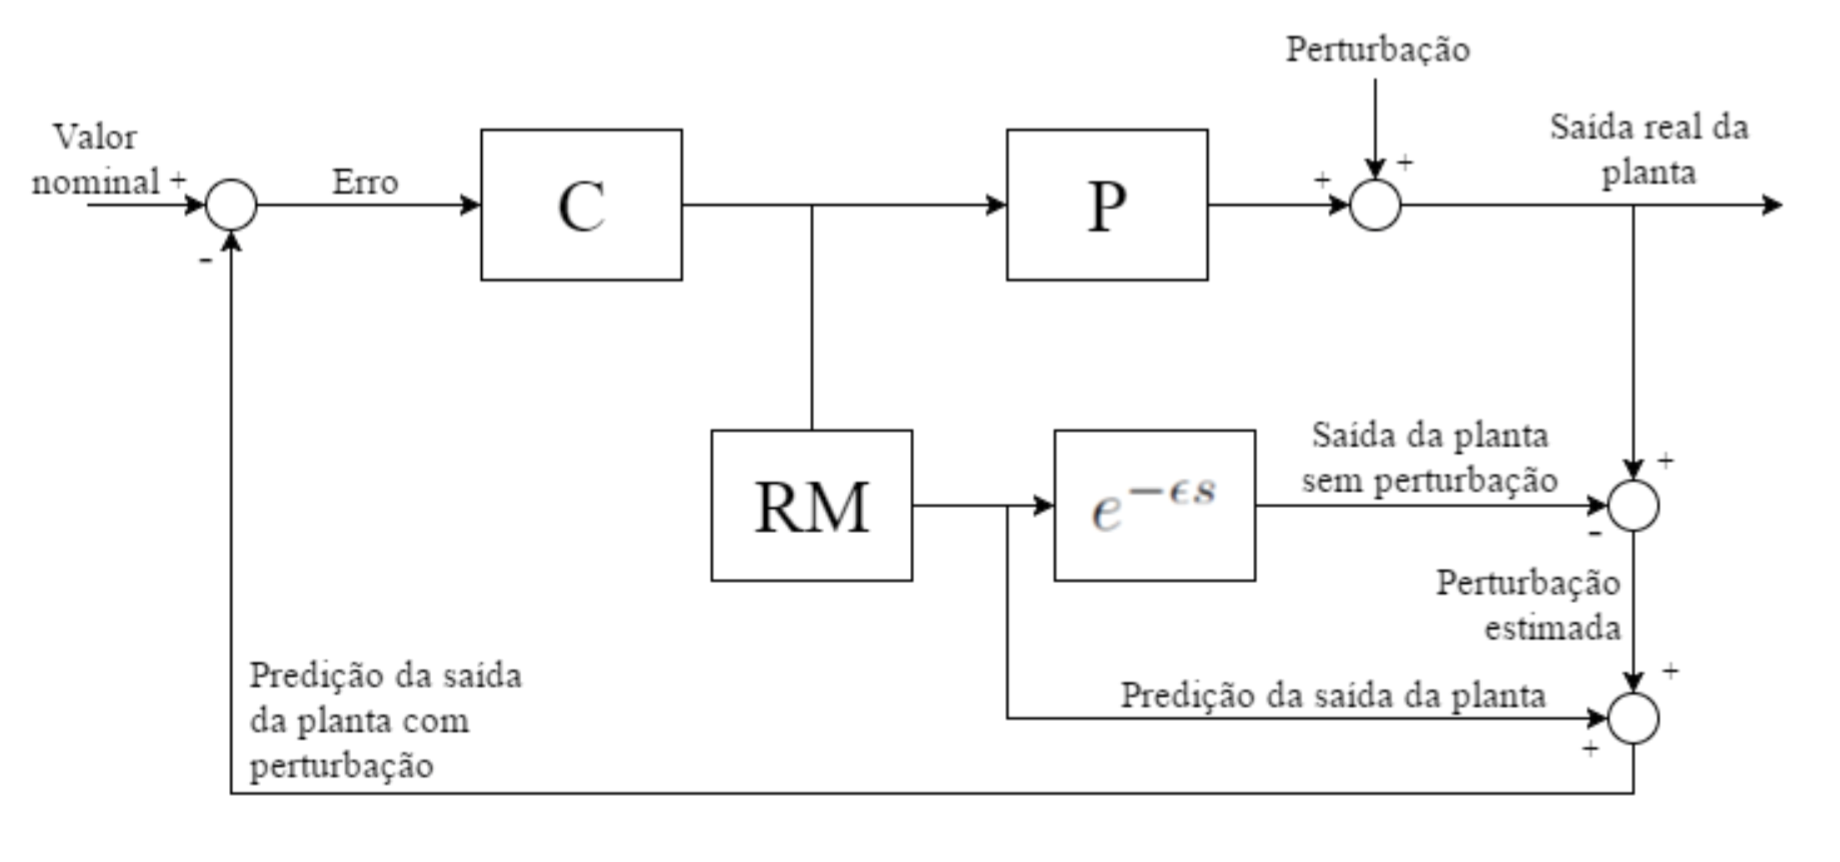
\includegraphics[width=.85\linewidth]{figs/fundamentos/preditorSmithSemKalman}
\caption{Estrutura básica do preditor de Smith \cite{rafaelMestrado}. \label{smith1}}
\end{figure}

A saída do modelo reduzido com atraso é uma estimativa da saída da planta desconsiderando-se efeitos de perturbação. Subtraindo-se essa saída com atraso da saída real da planta, tem-se uma estimativa de perturbação que, somada à saída sem atraso, resulta em uma predição da saída com perturbação; assim, a realimentação do preditor considera a perturbação sem ser influenciada pelo atraso.

A grande vantagem de se utilizar o preditor de Smith é que, dado o fato que o projeto pode ser realizado sobre o modelo reduzido sem atraso, podem ser utilizadas técnicas elementares de controle em espaço de estados, apresentadas na Seção \ref{SimpleControlSection}. Conhecendo-se o atraso $\epsilon$, e sabendo que o modelo reduzido é um sistema SISO invariante no tempo e controlável, ele pode ser representado em forma canônica de controle. De posse desse fato, pode-se montar uma nova estrutura para o preditor de Smith, confForme a Figura \ref{smith2} . Nessa estrutura, \textbf{P} é a planta, \textbf{C} é o controlador em malha fechada, \textbf{RM} é o modelo sem atraso e \textbf{KF} é um Filtrode Kalman, que utiliza a forma canônica de controle do sistema de forma a ter sua saída simplificada. O funcionamento do filtro será explicado adiante. 

Com essa nova estrutura, dada a linearidade do sistema, o princípio de superposição é válido; portanto, os problemas de planejamento e acompanhamento de trajetória podem ser tratados de forma separada. O preditor leva em consideração as referências de trajetória de topo, $u^{*} = \Upsilon_0 (L,t)$, e de trajetória de fundo, $y^{*} = \Upsilon_R (0,t)$. Desta forma, garante-se que a trajetória de fundo seja seguida, mesmo com a presença de perturbações.

\begin{figure}[!ht]
\centering
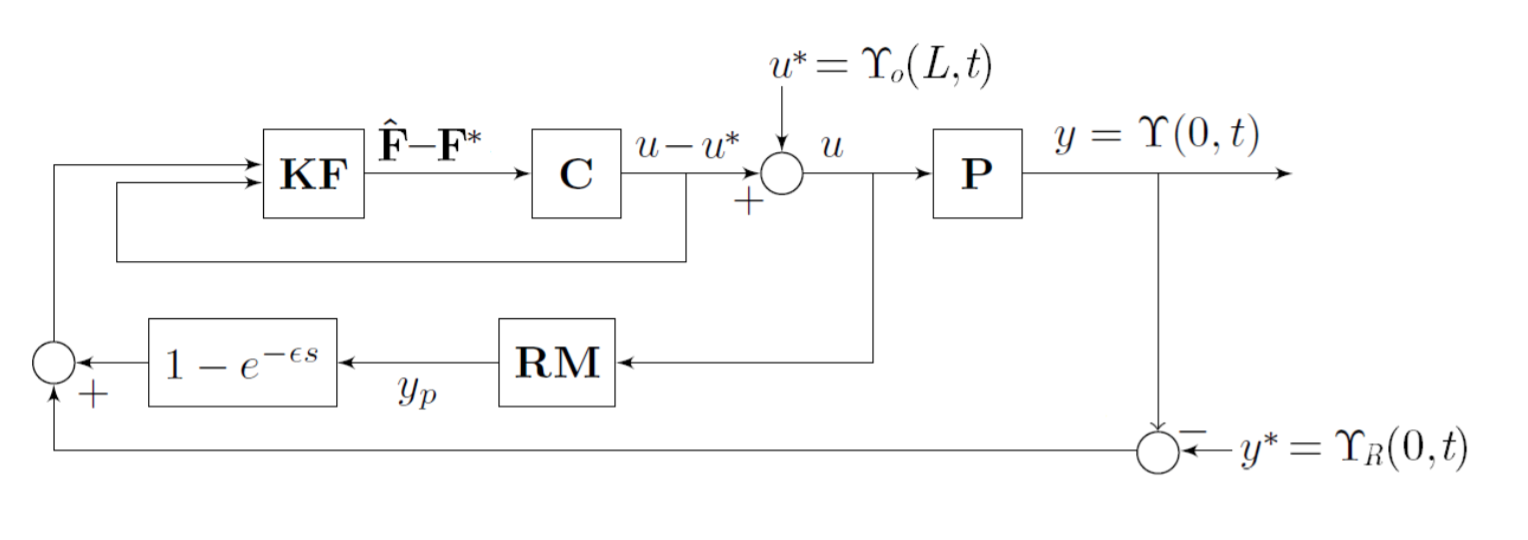
\includegraphics[width=.85\linewidth]{figs/fundamentos/preditorSmith}
\caption{Estrutura do preditor de Smith com filtro de Kalman e referências de topo e fundo \cite{rafaelMestrado}. \label{smith2}}
\end{figure}

Apesar de mencionadas as trajetórias de topo e fundo, dadas por $u^*$ e $y^*$, respectivamente, este trabalho não demonstra como elas foram calculadas. Foram utilizadas trajetórias determinadas por Rafael \cite{rafaelMestrado}. Essas trajetórias permitem um controle adequado em malha aberta na ausência de perturbações e uma referência suave para ser seguida em malha fechada. A seção de resultados irá apresentar essas trajetórias nos resultados de simulação e experimentais.

\subsection{Filtro de Kalman}
Uma estrutura essencial para um sistema de controle real é o filtro de Kalman. Esse filtro é capaz de estimar valores tanto para o processo quanto para o resultado, compensando os erros associados a ruídos de medição e à incerteza do modelo. Assumindo-se que os estados do sistema sejam observáveis, é possível projetar o \textbf{Filtro de Kalman}, que leva o nome do seu criador, Rudolf E. Kalman.

O Filtro de Kalman, também conhecido como observador ótimo, é responsável por estimar, utilizando uma estrutura de predição e correção, variáveis de estado não medidas de forma a se utilizar os resultados obtidos em uma dada estratégia de controle \cite{GoddardKalman}. O Filtro de Kalman original é aplicado, principalmente, em sistemas discretos no tempo, como o que foi obtido para este projeto por meio da redução modal. A Figura \ref{Kalman1} mostra um exemplo de processo no qual o filtro pode ser aplicado.
\begin{figure}[!ht]
\centering

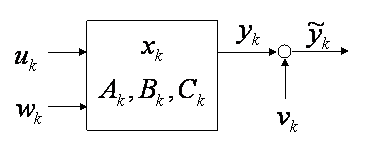
\includegraphics[width=.5\linewidth]{figs/kalman/kalman1}
\caption{Exemplo de estrutura de sistema discreto no tempo \cite{GoddardKalman}. \label{Kalman1}}
\end{figure}

O sistema representado pela Figura \ref{Kalman1} pode então ser representado por equações lineares, como se segue:
\begin{align}
	\label{KalmanEq1}
	x_k &= \mathbf{A_k} x_{k-1} + \mathbf{B_k} u_k + w_{k-1}, \\
	\label{KalmanEq2}
	y_k &= \mathbf{C_k} x_k, \\
	\label{KalmanEq3}
	\tilde{y}_k &= y_k + v_k.
\end{align}

No sistema representado pelas Equações \ref{KalmanEq1}-\ref{KalmanEq3}, as matrizes $\mathbf{A_k}$, $\mathbf{B_k}$ e $\mathbf{C_k}$ são as matrizes próprias do espaço de estados do sistema discreto; $x_k$ é o vetor de variáveis de estado, $y_k$ é a saída do processo e $\tilde{y}_k$ é uma medida da referida saída. As variáveis $w_k$ e $v_k$ são ruídos associados respectivamente ao processo e à medida. Suas covariâncias podem ser representadas por $\mathbf{Q_k}$ para o processo e $\mathbf{R_k}$ para a medida.

Dada a estrutura do sistema, o objetivo do uso do filtro de Kalman é estimar os dados do processo e a medida das saídas, dadas as entradas e as medições das saídas. A Figura \ref{Kalman2} mostra um esquema de uso do filtro, em que $\hat{x}_k$ e $\hat{y}_k$ são, respectivamente, as estimações das variáveis de estado e da saída.
\begin{figure}[!ht]
\centering
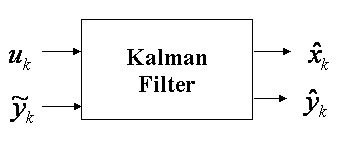
\includegraphics[width=.5\linewidth]{figs/kalman/kalman2}
\caption{Exemplo de estrutura de filtro de Kalman \cite{GoddardKalman}. \label{Kalman2}}
\end{figure}

O Filtro de Kalman é um algoritmo de dois passos: predição, em que o estado mais recente e a estimação do erro de covariância são projetados de forma a se computar o estado atual das variáveis de estado, e correção, onde o estado predito pelo primeiro passo é corrigido incorporando-se a medida mais recente do processo para se gerar uma nova estimação do estado \cite{GoddardKalman}. Matematicamente, a predição é dada por
\begin{align}
	\label{KalmanEq4} {\hat{x}_{k}}^{-} &= \mathbf{A_k} \hat{x}_{k-1} + \mathbf{B_k} u_k\;\mathrm{e} \\
	\label{KalmanEq5} \mathbf{{\hat{P}_{k}}^{-}} &= \mathbf{A_k}\mathbf{P_{k-1}}\mathbf{{A_k}^T} + \mathbf{Q_k},
\end{align}
 enquanto que a correção pode ser descrita por
\begin{align}
	\label{KalmanEq6} \mathbf{K_k} &= \mathbf{{\hat{P}_{k}}^{-}}\mathbf{{C_k}^T} {\left( \mathbf{C_k}\mathbf{{\hat{P}_{k}}^{-}}\mathbf{{C_k}^T} + \mathbf{R_k} \right)}^{-1}, \\
	\label{KalmanEq7} \hat{x}_k &= {\hat{x}_{k}}^{-} + \mathbf{K_k} \left( \tilde{y}_k - \mathbf{C_k}{\hat{x}_{k}}^{-} \right)\;\mathrm{e} \\
	\label{KalmanEq8} \mathbf{P_k} &= \left( \mathbf{I} - \mathbf{K_k}\mathbf{C_k}\right)\mathbf{{\hat{P}_{k}}^{-}}.
\end{align} 

Nas Equações \ref{KalmanEq4}-\ref{KalmanEq8}, $\mathbf{P_k}$ é uma estimação da covariância de erro da medição, enquanto $\mathbf{K_k}$ é denominado ganho de Kalman. Após os dois passos do algoritmo, $\hat{x}_k$ e $\mathbf{P_k}$ são preservados continuamente, de forma a serem utilizados na parte de predição no próximo instante de tempo \cite{GoddardKalman}.

No presente projeto, o filtro de Kalman é utilizado em conjunção com o controlador. Porém, é admitido um caso especial, em que as matrizes passadas para o filtro são discretizadas a partir do sistema contínuo escrito em forma canônica controlável. Nesse caso , $\hat{y}_k$ é diretamente dependente de uma das variáveis de estado, tornando o conjunto controlador-filtro mais simples de ser implementado, uma vez que é tomada a integral de uma variável de estado, apenas.


\section{Redes Utilizadas}
\subsection{DeviceNET}
DeviceNET é um protocolo de baixo nível da camada de aplicação, voltado a ambientes industriais \cite{dnetrta}. Ele suporta comunicação entre dispositivos de baixo nível, como sensores e atuadores, e dispositivos de alto nível, como o computador e o CLP \cite{devicenetrockwell}. Permite também uma rápida configuração entre dispositivos a \textit{byte}, suportando tanto dispositivos analógicos quanto digitais \cite{redytton}. As velocidades de transmissão são de até 500 kbps, sendo bem mais lenta que uma rede Ethernet.

No experimento, a rede DeviceNET é utilizada para a conexão entre o CLP e os sensores indutivos presentes na planta \cite{redytton}.  Para fins de detecção de fim-de-curso, será utilizado o modo digital dos sensores, uma vez que apenas é necessário verificar se o carrinho está na área de detecção do sensor. O módulo responsável pelo gerenciamento da rede DeviceNET é o 1756-DNB.

\subsection{Ethernet/IP}
A rede Ethernet/IP, introduzida em meados de 2001 pela ODVA (\textit{Open DeviceNet Vendor Association}) \cite{eipodva1}, é um tipo de rede Ethernet voltada ao ambiente industrial, seguindo o CIP, assim como o DeviceNET \cite{eiprta}. É uma rede robusta, organizada segundo o modelo OSI de 7 camadas, que permite conexão com dispositivos conectados a redes Ethernet padrão. Ela permite a passagem de dados via pacotes TCP ou UDP e é indicada em aplicações que exigem uma transferência rápida e confiável de dados, principalmente em aplicações de tempo real \cite{eiprockwell}.

No presente experimento, a rede Ethernet/IP é utilizada para receber dados de inspeção da câmera, notadamente a posição horizontal da bola de isopor presa ao barbante. Além disso, ela é utilizada na transferência de programas entre o computador e o CLP (através do módulo Ethernet 1756-ENBT/A), uma vez que ela provê uma comunicação mais rápida do que o RS-232. O computador também pode enviar e receber dados por essa rede utilizando OPC.

Por meio do Ethernet, em particular, utilizou o padrão OPC - \textit{OLE for Process Control}. Esse padrão, cuja primeira versão foi lançada em 1996, é voltado ao ambiente industrial. O padrão é responsável, em termos gerais, pela troca confiável de dados entre o CLP, computadores e outros dispositivos. Ele abstrai o protocolo de rede utilizado no CLP (seja ModBus, Profibus, Ethernet/IP, etc.) em uma interface padrão de forma que sistemas HMI/SCADA possam se comunicar com um ``intermediário'' que converta as operações de dados de OPC em operações específicas de dispositivo e vice-versa \cite{OPCFoundation1}. 

Uma das características do OPC é permitir a troca de dados entre o CLP e o computador por meio de um sistema \textit{server/client}. No presente projeto, o \textit{server} é disponibilizado pelo \textit{software} RSLinx, enquanto que o cliente é um programa desenvolvido externamente ao CLP. Para esse programa, foi escolhida a linguagem Python; a razão da escolha de tal linguagem foi, além da existência de módulos programados por terceiros para lidar com a rede OPC, o fato de Python ter outros módulos que facilitam a implementação de controladores e ser razoavelmente rápido.

Para se programar o \textit{client} OPC em Python, foi utilizado o módulo OpenOPC \cite{OpenOPC}. Esse módulo é bem simples de se utilizar; as funções de trocas de dados OPC são abstraídas de modo a utilizar elementos simples da linguagem, como o uso de dicionários, que são estruturas nas quais se relacionam chaves com valores. 

A utilização do OPC permite realizar um sistema de controlador no qual o computador auxilia nos cálculos, assim como permite salvar dados do CLP para posterior desenho dos gráficos.

\section{Programação do CLP}
\subsection{Visão geral}
Programação, em termos gerais, é aplicada na resolução de problemas. Em particular, a programação de CLPs busca resolver, no âmbito industrial, problemas relacionados à automação de processos. Essa resolução de problemas segue uma metodologia, de forma a se direcionar o projeto. Antes de se proceder à programação, faz-se necessário seguir os seguintes passos \cite{rockwellAutomation}:
\begin{enumerate}
  \item Descrição do problema;
  \item Detalhamentos e melhoria do processo;
  \item Especificação dos atuadores e sensores da planta;
  \item Elaboração do algoritmo;
  \item Representação gráfica do algoritmo, quando aplicável;
  \item Esquema funcional, quando aplicável;
  \item Seleção dos módulos do controlador;
  \item Programação, utilizando linguagens suportadas.
\end{enumerate}

Ao se programar o CLP, deve-se ter em conta que o controlador executa sempre três ciclos \cite{rockwellAutomation}:
\begin{enumerate}
  \item \textit{Scan} de Entrada: Ciclo em que o controlador recebe todos os dados de seus módulos de entrada;
  \item \textit{Scan} do Programa: Ciclo em que o controlador processa as entradas recebidas e gera as saídas;
  \item \textit{Scan} de Saída: Ciclo em que o controlador envia os dados de saída para os módulos de saída.
\end{enumerate}

Para o presente experimento, entre as várias linguagens disponíveis para CLPs, foram selecionadas duas: uma linguagem gráfica, o \textbf{\textit{ladder}}, e uma linguagem textual, o \textbf{texto estruturado}. Ambas foram selecionadas por serem linguagens muito utilizadas, normalmente rápidas e que ocupam pouca memória, ao contrário de linguagens como SFC (\textit{Sequential Flow Chart}) e FBD (\textit{Function Block Diagram}), que também poderiam ser utilizadas.

\subsection{Linguagem \textit{ladder}}
\subsubsection{Introdução ao \textit{ladder}}
A linguagem \textit{ladder} é uma linguagem de programação gráfica, e uma das primeiras a ser utilizada na programação de CLPs. Seu nome vem do inglês \textit{ladder}, que significa escada; nome dado em razão dos programas, ao serem feitos, assumirem a forma de uma escada, e lidos de cima para baixo (movimento de descida). Essa linguagem foi estruturada de forma a ter uma simbologia semelhante à de um diagrama de conexão de relés, que eram utilizados em indústrias antes do CLP.

Todo programa \textit{ladder} possui duas linhas verticais e, entre elas, uma ou mais linhas horizontais nas quais são especificados os comportamentos do programa. A linguagem possui várias instruções, em sua maioria comuns entre diferentes tipos de CLP. A Tabela \ref{ladder1} mostra as principais instruções utilizadas em \textit{ladder}, utilizando a sintaxe presente no \textit{software} RSLogix5000.

\begin{table}[!ht]
  \centering
  \caption{Principais instruções \textit{ladder} \label{ladder1}}
  \begin{tabularx}{\textwidth}{|>{\bfseries}l|l|X|}
    \hline
    Desenho da Instrução & Nome da Instrução & Descrição \\ \hline
    -( )- & OTE & Atualiza variável booleana de acordo com a condição da linha \\ \hline
    -(L)- & OTL & Atribui valor verdadeiro à variável booleana se a linha for alimentada \\ \hline
    -(U)- & OTU & Atribui valor falso à variável booleana se a linha for alimentada \\ \hline
    -[ ]- & XIC & Examina se a variável possui valor verdadeiro \\ \hline
    -[/]- & XIO & Examina se a variável possui valor falso \\ \hline
  \end{tabularx}
\end{table}

\subsubsection{Instruções específicas}
No presente trabalho, a presença do servomotor exige uma lógica e entradas que não são booleanas, ou seja, que não podem ser tratadas pelos operadores descritos na Tabela \ref{ladder1}. Portanto, faz-se necessário o uso de novas instruções, diretamente relacionadas com o movimento do atuador. Tais instruções são conhecidas, dentro do RSLogix5000, como \textit{Motion Control Instructions}, ou instruções de controle de movimento. A Tabela \ref{ladder2} mostra as instruções desse tipo utilizadas no experimento.

\begin{table}[!ht]
  \centering
  \caption{Principais instruções de controle de movimento em \textit{ladder} \label{ladder2}}
  \begin{tabularx}{\textwidth}{|>{\bfseries}l|l|X|}
    \hline
    Nome da Instrução & Sigla & Função \\ \hline
    \textit{Motion Servo On} & MSO & Inicializa o servomotor, travando a esteira. \\ \hline
    \textit{Motion Axis Jog} & MAJ & Envia comandos de velocidade e sentido de rotação ao motor, executando sua movimentação. \\ \hline
    \textit{Motion Axis Stop} & MAS & Interrompe a movimentação do motor; a esteira permanece travada. \\ \hline
    \textit{Motion Servo Off} & MSF & 
    Desativa o servomotor, destravando a esteira e permitindo a movimentação manual do carrinho.\\ \hline
  \end{tabularx}
\end{table}

As funções descritas pela Tabela \ref{ladder2} lidam com outros tipos de variáveis, como números reais, para a velocidade do motor, e até mesmo estruturas que o \textit{software} RSLogix cria para armazenar informações sobre os eixos e o controle feito pelas instruções. Tais parâmetros podem ser alterados dentro dos blocos das funções. A Figura \ref{motionladder1} mostra um exemplo de tais instruções.

\begin{figure}[!ht]
  \centering
    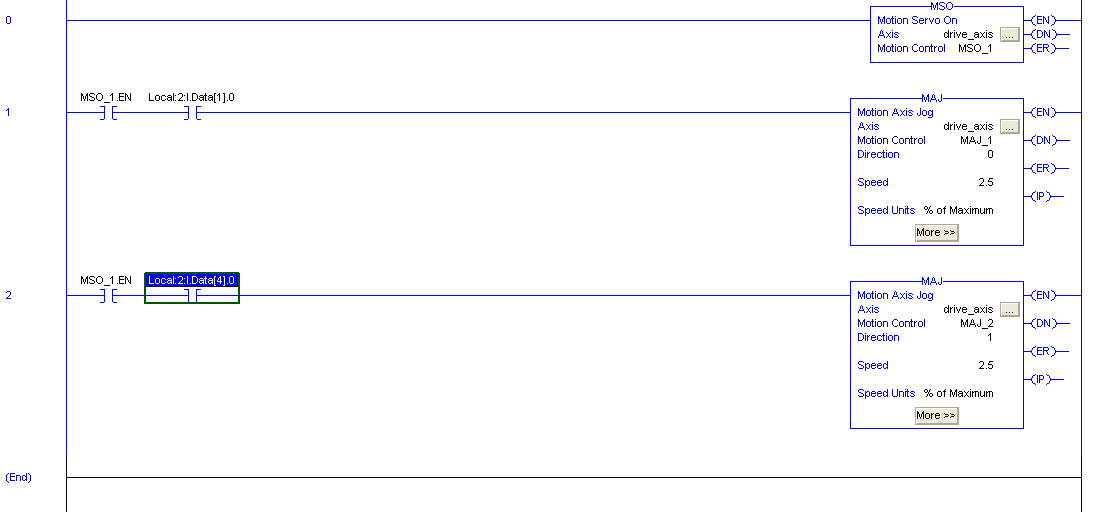
\includegraphics[width=0.6\textwidth]{figs/fundamentos/motionladder}
    \caption{Exemplo de programa \textit{ladder} com instruções de movimentação.\label{motionladder1}}
\end{figure}

\subsection{Texto Estruturado}
\subsubsection{Visão geral do texto estruturado}
Além de \textit{ladder}, que é uma linguagem gráfica, o CLP utilizado no experimento também suporta uma linguagem puramente textual, o texto estruturado. Essa linguagem é uma linguagem sequencial, que lembra muito linguagens como BASIC, C ou Pascal. Cada comando é executado em sequência, salvo em caso de desvios (estruturas do tipo \textit{if-then-else}) ou repetições (\textit{loops}, estruturas do tipo \textit{while}).

Em relação ao \textit{ladder}, o texto estruturado possui vantagens e desvantagens. A principal vantagem é o fato do texto estruturado se assemelhar às linguagens de programação mais utilizadas; isso torna tal linguagem de fácil aprendizado. Além disso, por ser texto, caso seja necessário editar muitos parâmetros cuja criação seja de fácil automação, um programa auxiliar escrito em linguagens de programação genéricas pode simplificar a geração do texto estruturado. Porém, uma desvantagem do texto em relação ao \textit{ladder} reside nas funções de movimentação, uma vez que, ao contrário do \textit{ladder}, o texto estruturado não dá uma indicação clara associando um valor e a variável que ele representa, além da ordem dos parâmetros. Isso torna o uso de funções como MAJ (vide Tabela \ref{ladder2}) um pouco mais complicado em texto estruturado.

\subsubsection{Instruções de movimentação do motor para o texto estruturado}
Assim como o \textit{ladder}, o texto estruturado permite o uso das funções descritas na Tabela \ref{ladder2}. A sintaxe de uso dessas funções lembra muito a sintaxe da linguagem C, com o nome da função e uma lista de parâmetros válidos separados por vírgulas. A seguir, um exemplo de uso:
 
\begin{lstlisting}
/**
* MSO: ativa o servo cujo eixo eh descrito
* por drive_axis; informacoes de controle
* sao gravadas em MSO_1
*/
  MSO(drive_axis,MSO_1);
/* Atribui o valor 0.0 ao primeiro elemento do array speed */
  speed[0] := 0.0; 
/* Atribui 1 para dataInitialized */
  dataInitialized := 1;
\end{lstlisting}

Nota-se que o código apresentado, a menos da operação de atribuição, possui uma sintaxe muito semelhante à de C. A função MSO acima recebe dois parâmetros, assim como em \textit{ladder}; porém, a única indicação de como os parâmetros se comportam é a ordem com que eles são colocados; no caso de MSO, o 1º parâmetro é o eixo que será inicializado, e o 2º parâmetro é uma \textit{tag} que guarda as informações de controle executadas por MSO.


\section{Parâmetros para gerar trajetórias}

Fabrício et al \cite{fabricioIFAC} desenvolveram um método para gerar trajetórias \textit{offline} (controle malha aberta) assim como \textit{online} (controle malha fechada). Para se utilizar do método, é necessário ter parâmetros do sistema. Se fosse necessário simular ou controlar o sistema real, utilizariam-se os dados da Tabela \ref{escalaReal}, conforme cita Rédytton \cite{redytton}.

\begin{table}[!ht]
\parbox{.45\linewidth}{
\centering
\caption{Dados para simulação em escala real\label{escalaReal} \cite{redytton}}
\vspace{0.5cm}
	\begin{tabular}{|c|c|}
	\hline
		\multicolumn{2}{|c|}{\textbf{Dados do Riser}}\\ \hline
		Diâmetro externo & $0.55\mathrm{m}$\\ \hline
		Diâmetro interno & $0.5\mathrm{m}$ \\ \hline
		Comprimento & $2000\mathrm{m}$ \\ \hline
		Módulo de Elasticidade & $200 \mathrm{GPa}$\\ \hline
		Densidade &  $7860\mathrm{kg}/\mathrm{m}^3$\\ \hline
		\multicolumn{2}{|c|}{\textbf{Dados do fluido (Água)}}\\ \hline
		Densidade do fluido &  $1000\mathrm{kg}/\mathrm{m}^3$\\ \hline
		Viscosidade dinâmica & $10^3 \mathrm{Pa}\cdot \mathrm{s}$ \\ \hline
	\end{tabular}
}
\hfill
\parbox{.45\linewidth}{
	\caption{Dados para simulação em escala laboratorial\label{escalaLaboratorial}}
	\centering
	\vspace{0.5cm}
	\begin{tabular}{|c|c|}
		\hline
			\multicolumn{2}{|c|}{\textbf{Dados da Massa na Ponta - Isopor}} \\ \hline
			Diâmetro Externo & $30.6\mathrm{mm}$\\ \hline
			Densidade & $10\mathrm{kg}/\mathrm{m}^3$ \\ \hline
			\multicolumn{2}{|c|}{\textbf{Dados do Riser (Barbante)}}\\ \hline
			Diâmetro externo & $2\mathrm{mm}$\\ \hline
			Diâmetro interno & $0\mathrm{mm}$ \\ \hline
			Comprimento & $82\mathrm{cm}$ \\ \hline
			Módulo de Elasticidade & $2.1 \mathrm{MPa}$\\ \hline
			Densidade &  $191\mathrm{kg}/\mathrm{m}^3$\\ \hline
			\multicolumn{2}{|c|}{\textbf{Dados do fluido (Ar)}}\\ \hline
			Densidade do fluido &  $1.2754\mathrm{kg}/\mathrm{m}^3$\\ \hline
			Viscosidade dinâmica & $17.2\cdot 10^6 \mathrm{Pa}\cdot \mathrm{s}$ \\ \hline
		\end{tabular}
}

\end{table}

Como é importante se validar o sistema, mas nem sempre isso é possível em escala real devido ao altíssimo custo e aos riscos envolvidos, é necessário um conjunto equivalente de parâmetros tais que permita validar o sistema em escala laboratorial. O \textit{riser} é representado por um barbante e a água é trocada pelo ar. Uma massa na ponta foi adicionada e os dados resultantes estão na Tabela \ref{escalaLaboratorial}. Esses são os dados que serão utilizados para os experimentos, assim como as Tabelas \ref{constanteBarbante} e \ref{constanteIsopor}.


%Resultados
%TCIDATA{LaTeXparent=0,0,relatorio.tex}
\chapter{Resultados\label{chap:Resultados}}

% Resumo opcional. Comentar se não usar.
\resumodocapitulo{Este capítulo apresenta os procedimentos experimentais realizados e seus resultados.}


\section{Câmera}

Os problemas com a câmera se resumiram a configuração da rede, calibração e programação, sendo o mais difícil esse último.

\subsection{Configuração da Rede}
A câmera estava com um \textit{firmware} antigo e foi necessário obter o arquivo 2014R1B PresencePLUS Firmware\footnote{Atualização de Firmware da Câmera - \url{http://info.bannerengineering.com/_dav/cs/idcplg?IdcService=GET_FILE&RevisionSelectionMethod=LatestReleased&dDocName=B_4170042}. Acesso em 29/11/2015.} que é o programa de atualização da \textit{Banner Engineering} para esta câmera. Bastou executá-lo no computador, estando a câmera conectada ao \textit{switch} do laboratório assim como o computador estava, ambos por cabos Ethernet. Antes desta atualização, o \textit{software} da câmera não permitia selecionar a opção Ethernet/IP de forma a permitir utilizar o módulo Ethernet/IP do CLP.

Uma vez atualizado o \textit{firmware}, foi obtido o arquivo EDS\footnote{Arquivo EDS disponível em \url{http://www.bannerengineering.com/en-US/products/sub/78\#ui-tabs-37}. Acesso em 29/11/2015.} da câmera que foi então integrado ao \textit{software} da Rockwell no computador por meio do programa XXXX da própria Rockwell. %TODO Qual o programa de upar o EDS?

Após os procedimentos anteriores, adiciona-se a câmera como um módulo genérico usando o \textit{software} RSLogix, conforme instruções da Banner Engineering \cite{presencePlusEthernetIP}.
%TODO colocar procedimento de configuração da câmera para deixar do jeito que nós fizemos, utilizando figuras (print screen's) e falando dos números de Assembly
\subsection{Calibração}

%TODO Pegar printscreens do programa que roda na câmera
A câmera permite fazer medidas de distâncias em \textit{pixels}. De forma a se converter essa distância para milímetros, uma barra de alumínio com marcas e tamanho conhecido é utilizada. É importante primeiro calibrar o sistema, para se saber se há deformação de pixels significante ao longo da distância de interesse, nomeadamente o tamanho da barra de alumínio sendo utilizada, cerca de $532$mm. No PresencePlus P4 GEO 1.3, um programa é feito, com imagem de referência conforme Figura ..., que usa várias ferramentas de detecção de borda para identificar as posições de cada uma das marcas pretas da barra.  Seis marcas foram feitas e a Tabela \ref{relacoesmmpx} apresenta os resultados para cada seção. A distância entre duas marcas é de 10cm, com exceção da distância entre P0 e PEND que é o comprimento total da barra.
%TODO - obter imagem de referência e mencionar no parágrafo acima

\begin{table}[!ht]
\centering
\caption{Relações mm/px para diferentes seções da barra de alumínio \label{relacoesmmpx}}
	\begin{tabular}{|c|c|c|c|}
	\hline
		Seção 1 & Seção 2 & Distância (px) & mm/px\\ \hline
		P0 & P10 & 160 & 0.625\\ \hline
		P10 & P20 & 173 & 0.578\\ \hline
		P20 & P30 & 176 & 0.568\\ \hline
		P30 & P40 & 173 & 0.578\\ \hline
		P40 & P50 & 163 & 0.613\\ \hline
		P0 & PEND & 893 & 0.596\\ \hline
	\end{tabular}
\end{table}

O maior desvio da quantidade de milímetros por \textit{pixel} das seções em relação à da barra inteira é de aproximadamente 4.93\%. Há algumas imprecisões na maneira como os traços foram desenhados e é possível que o erro seja menor.

\subsection{Programação}
A programação da câmera inicia obtendo uma imagem de referência e adicionando-se ferramentas de detecção de pontos de interesse. Também é possível adicionar ferramentas que fazem operações matemáticas assim como enviam dados pela rede, o que é essencial para comunicar com o CLP.

%TODO colocar um exemplo de programação, dando algumas imagens de referência, deve ser do programa que usamos pra fechar a malha

\section{Calibração do Servomotor\label{calibracaoServomotorSecao}}

O RSLogix tem o bloco \texttt{MAJ} \textendash{} \textit{Motion Axis Jog} \textendash{} que permite alterar a velocidade do motor enquanto ele se movimenta. No entanto, o bloco espera que a entrada seja do tipo $[\mathrm{u}/\mathrm{s}$ ao invés de alguma unidade no SI tal como $[\mathrm{mm}/\mathrm{s}]$. Devido a isso, foi necessária uma calibração do sistema. Nela, anotou-se a posição inicial $x_0$ e a posição final $x_f$, ambas em milímetros, e definia-se um tempo $\Delta t$ no qual o carrinho se movimentaria a uma velocidade $v$ em $[\mathrm{u}/\mathrm{s}]$. Daí, calculava-se a velocidade em $[\mathrm{mm}/\mathrm{s}]$ com esses dados e tirou a média de alguns ensaios para se obter o valor de uma unidade, que é aproximadamente $71.32\mathrm{mm}$. Os dados de calibração estão na Tabela \ref{calibracaoServomotor}.

\begin{table}[!ht]
\centering
\caption{Dados de calibração do servomotor, média obtida é de 71.32 mm/unidade\label{calibracaoServomotor}}
\begin{tabular}{|c|c|c|c|c|c|}
\hline
	$x_0$ - [mm] & $x_f$ - [mm] & $\Delta t$ - [s] & Velocidade - [u/s] & Velocidade - [mm/s] & mm/u\\ \hline
2 &	71.8  &	2   &	0.5 &	34.9   & 	69.8\\ \hline
6 & 76.1  &	2   &	0.5 &	35.05  &	70.1\\ \hline
6 &	188	  &  5   &	0.5	&   36.4   &	72.8\\ \hline
6 &	185   &	2.5 &	1	& 	71.6   &	71.6\\ \hline
6 &	77    &	10  &	0.1	&   7.1    &	71\\ \hline
6 &	296.5 &	20	&   0.2 & 	14.525 &	72.625\\ \hline\end{tabular}
\end{table}

\section{Malha aberta}

O planejamento de trajetória em malha aberta e malha fechada para o \textit{riser} que está sendo utilizado neste trabalho foi desenvolvido por Fabrício et al \cite{fabricioIFAC}, conforme mencionado anteriormente. Um programa em MATLAB foi escrito e gerou trajetórias de excursão pré-definida. Rédytton \cite{redytton} testou o sistema para uma excursão de cerca de 1m, que é maior que o tamanho do barbante ($82\mathrm{cm}$) conforme apresentado na Tabela \ref{escalaLaboratorial}. No entanto, seu trabalho não utilizou uma massa de isopor na ponta, daí existirá uma diferença entre os resultados. Observe que, em malha aberta, deixou-se o ar condicionado da sala desligado, pois isto seria uma perturbação.

\subsection{Excursão de 30cm}
O primeiro teste em malha aberta testou a trajetória de posição da Figura \ref{DeslocamentoT1}. Conforme Rédytton \cite{redytton} mencionou em seu trabalho, utilizar os módulos de posição é mais lento do que utilizar módulos de velocidade para seguir essa trajetória. Desta forma, optou-se por usar diferenças finitas para derivar essa trajetória, resultando na Figura \ref{VelocidadeT1}. 

\begin{figure}[!htb]
    \centering
    \begin{minipage}{.45\textwidth}
        \centering
        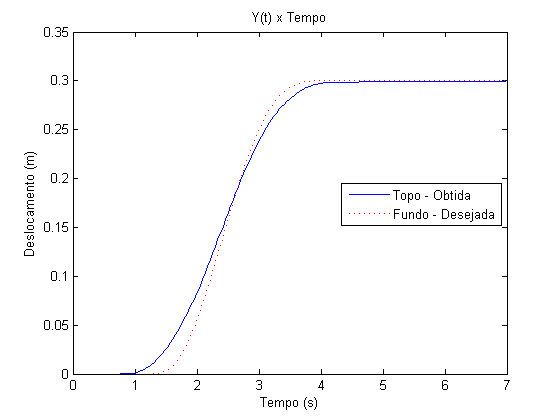
\includegraphics[width=1\linewidth]{figs/resultados/malha_aberta_1/DeslocamentoT1}
        \caption{Referência de Posição para Excursão de 30cm}
        \label{DeslocamentoT1}
    \end{minipage}%
    \hspace{0.1cm}
    \begin{minipage}{0.45\textwidth}
        \centering
        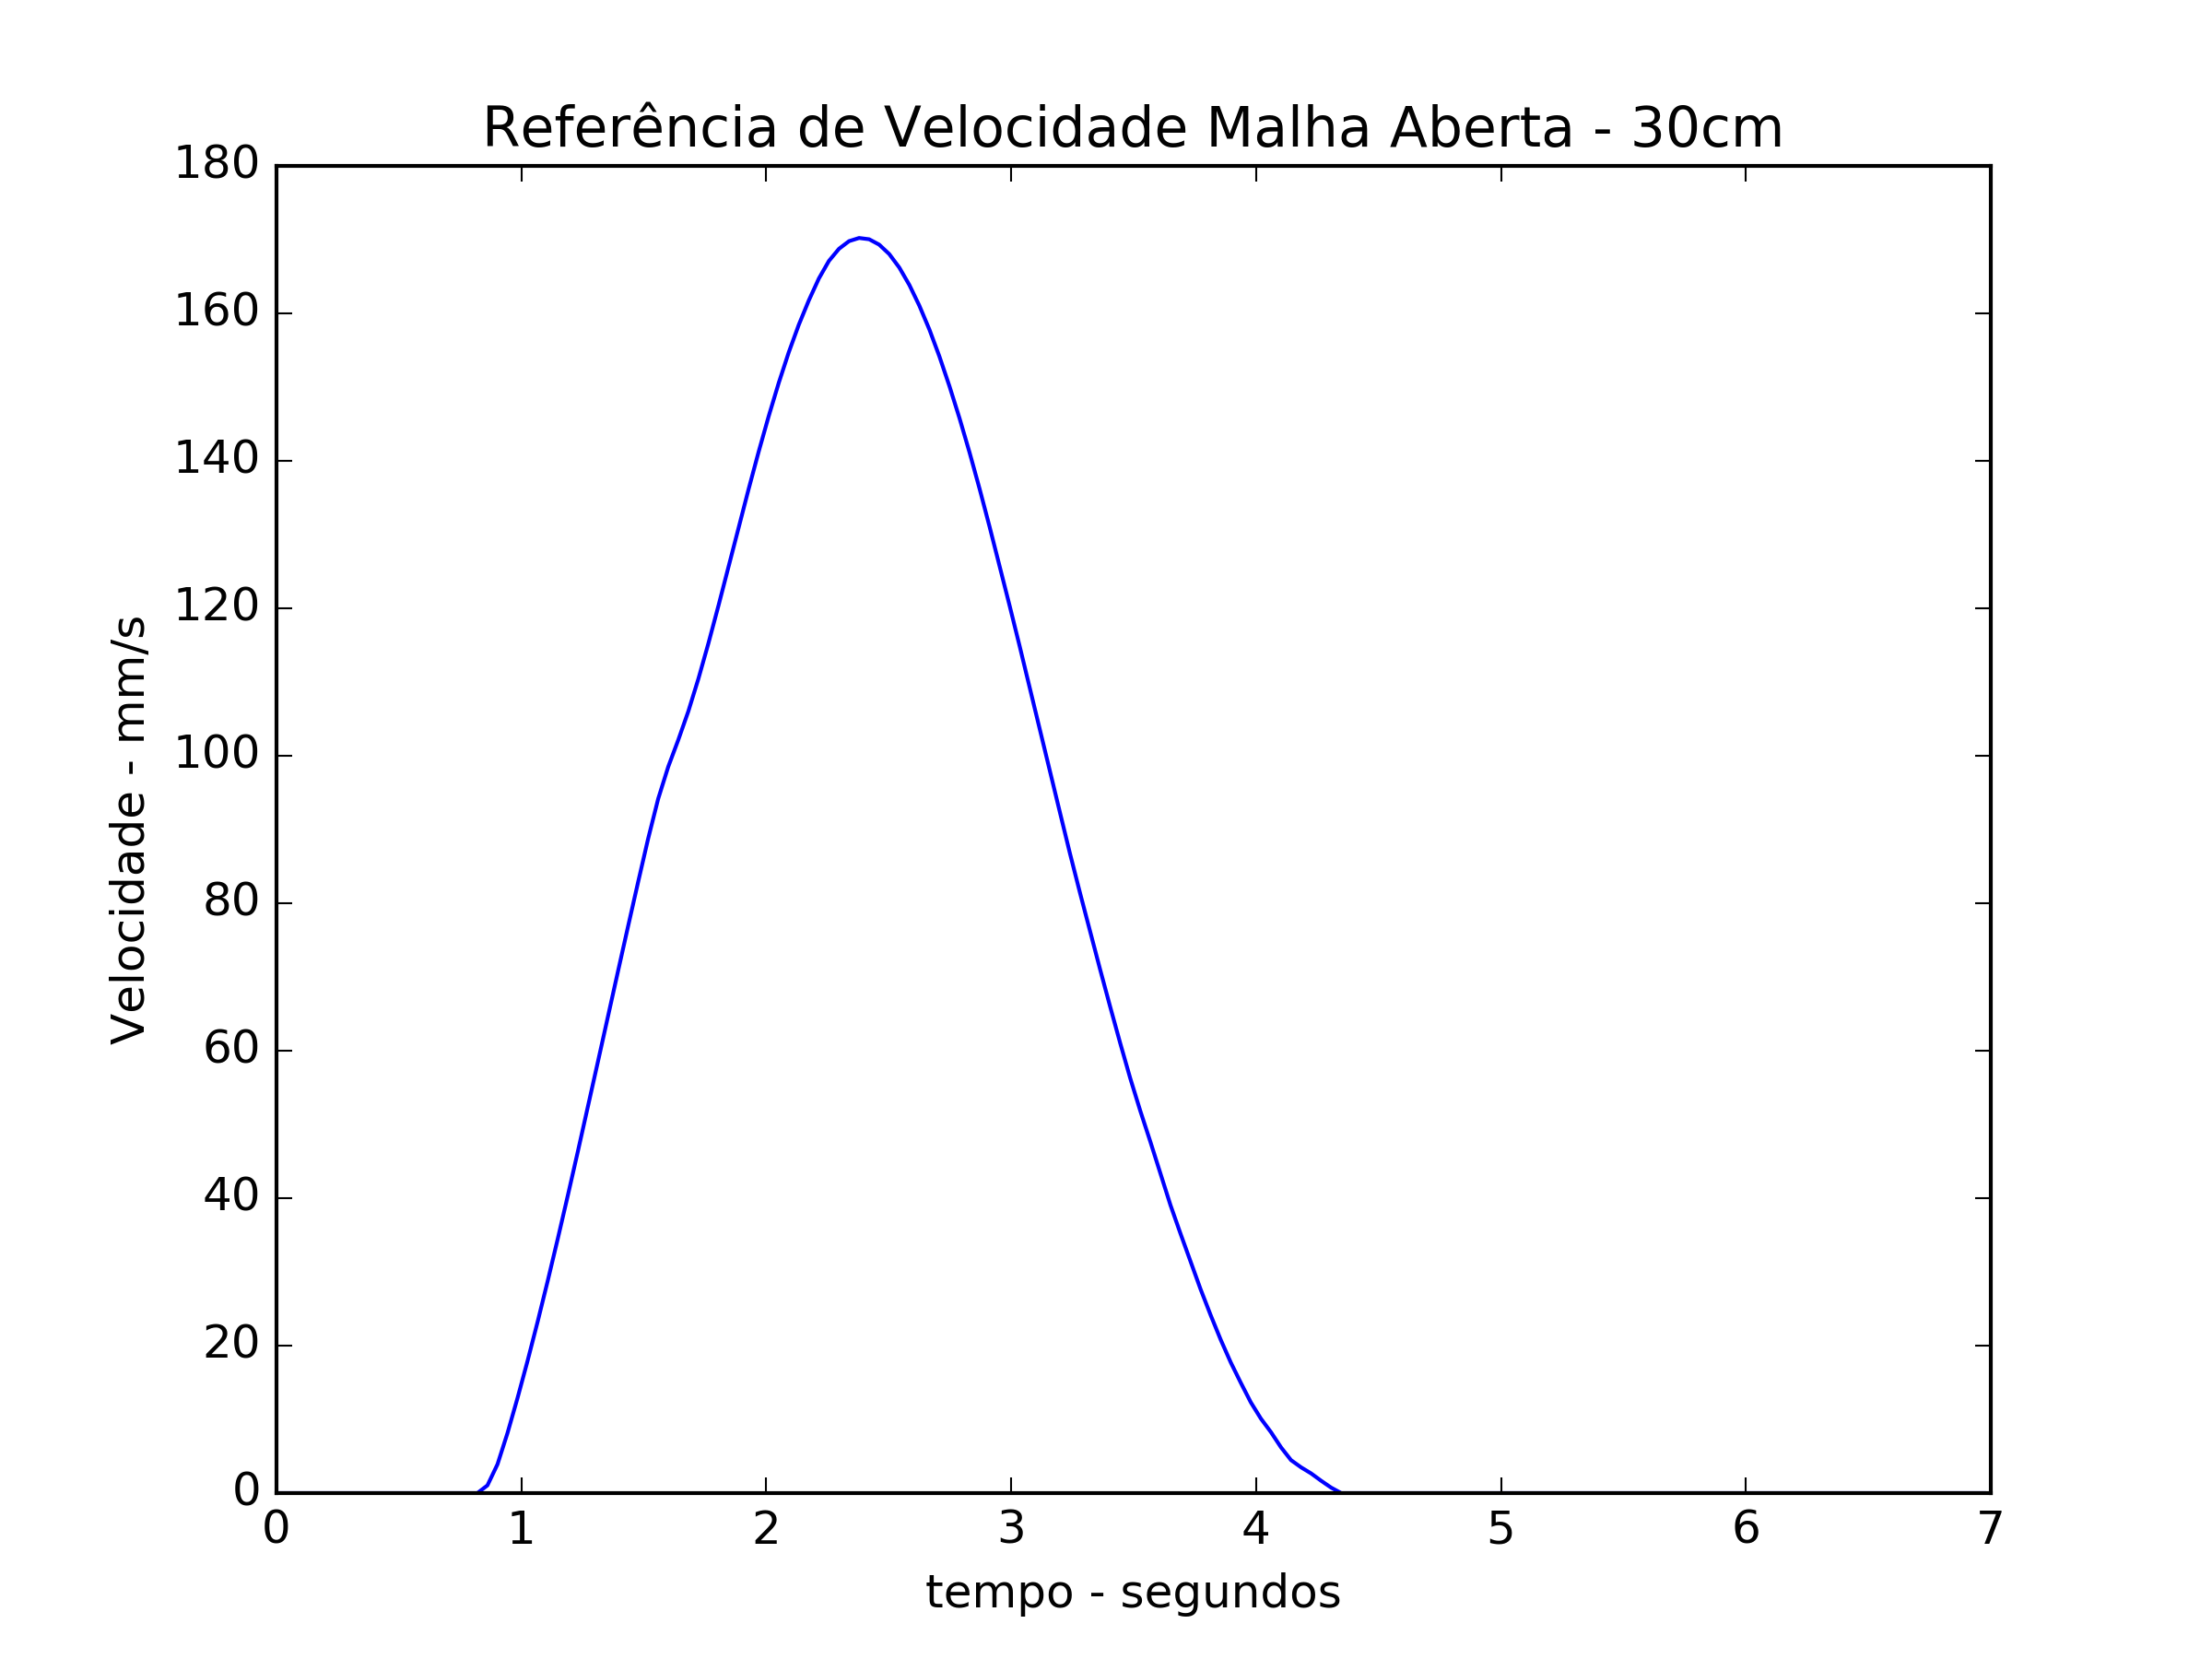
\includegraphics[width=1\linewidth]{figs/resultados/malha_aberta_1/VelocidadeT1}
        \caption{Referência de Velocidade para Excursão de 30cm}
        \label{VelocidadeT1}
    \end{minipage}
\end{figure}

Com um período de cerca de 41ms, uma tarefa eventual executava no CLP, aplicando um certo valor de velocidade ao carrinho. A câmera leu os valores de posição cada vez que a tarefa iniciava e o software RSLogix desenhou os dados, que podem ser observados na Figura \ref{trajetoriaObtidaModelada}. Observa-se que a posição evolui de forma bem suave. Para se realizar uma comparação, calculou-se o tempo que o carrinho se move na trajetória ($\Delta t$, tempo no qual a velocidade não é nula) e calculou-se $\overline{v} = \frac{\Delta x}{\Delta t}$. No caso presente, $\Delta x = 30\mathrm{cm}$ e $\Delta t \approx 3\mathrm{s}$ (veja Figura \ref{VelocidadeT1}), resultando em $\overline{v} = 100\mathrm{mm}/\mathrm{s}$. A Figura \ref{trajetoriaObtidaVConstante} apresenta esses resultados e observa-se várias oscilações quando o carrinho para, diferente do caso anterior.

Vídeos foram criados para cada um destes casos e estão disponíveis no YouTube{\sffamily\textregistered\textcopyright}, tanto para a trajetória modelada\footnote{Controle Malha Aberta Modelado, 30cm - \url{https://youtu.be/lKajz6LyauE}. Acesso em 29/11/2015.} quanto para a trajetória com velocidade constante\footnote{Controle Malha Aberta a Velocidade Constante, 30cm - \url{https://youtu.be/tB0TsmBcfVg}. Acesso em 29/11/2015.}.

\begin{figure}[!htb]
    \centering
    \begin{minipage}{.45\textwidth}
        \centering
        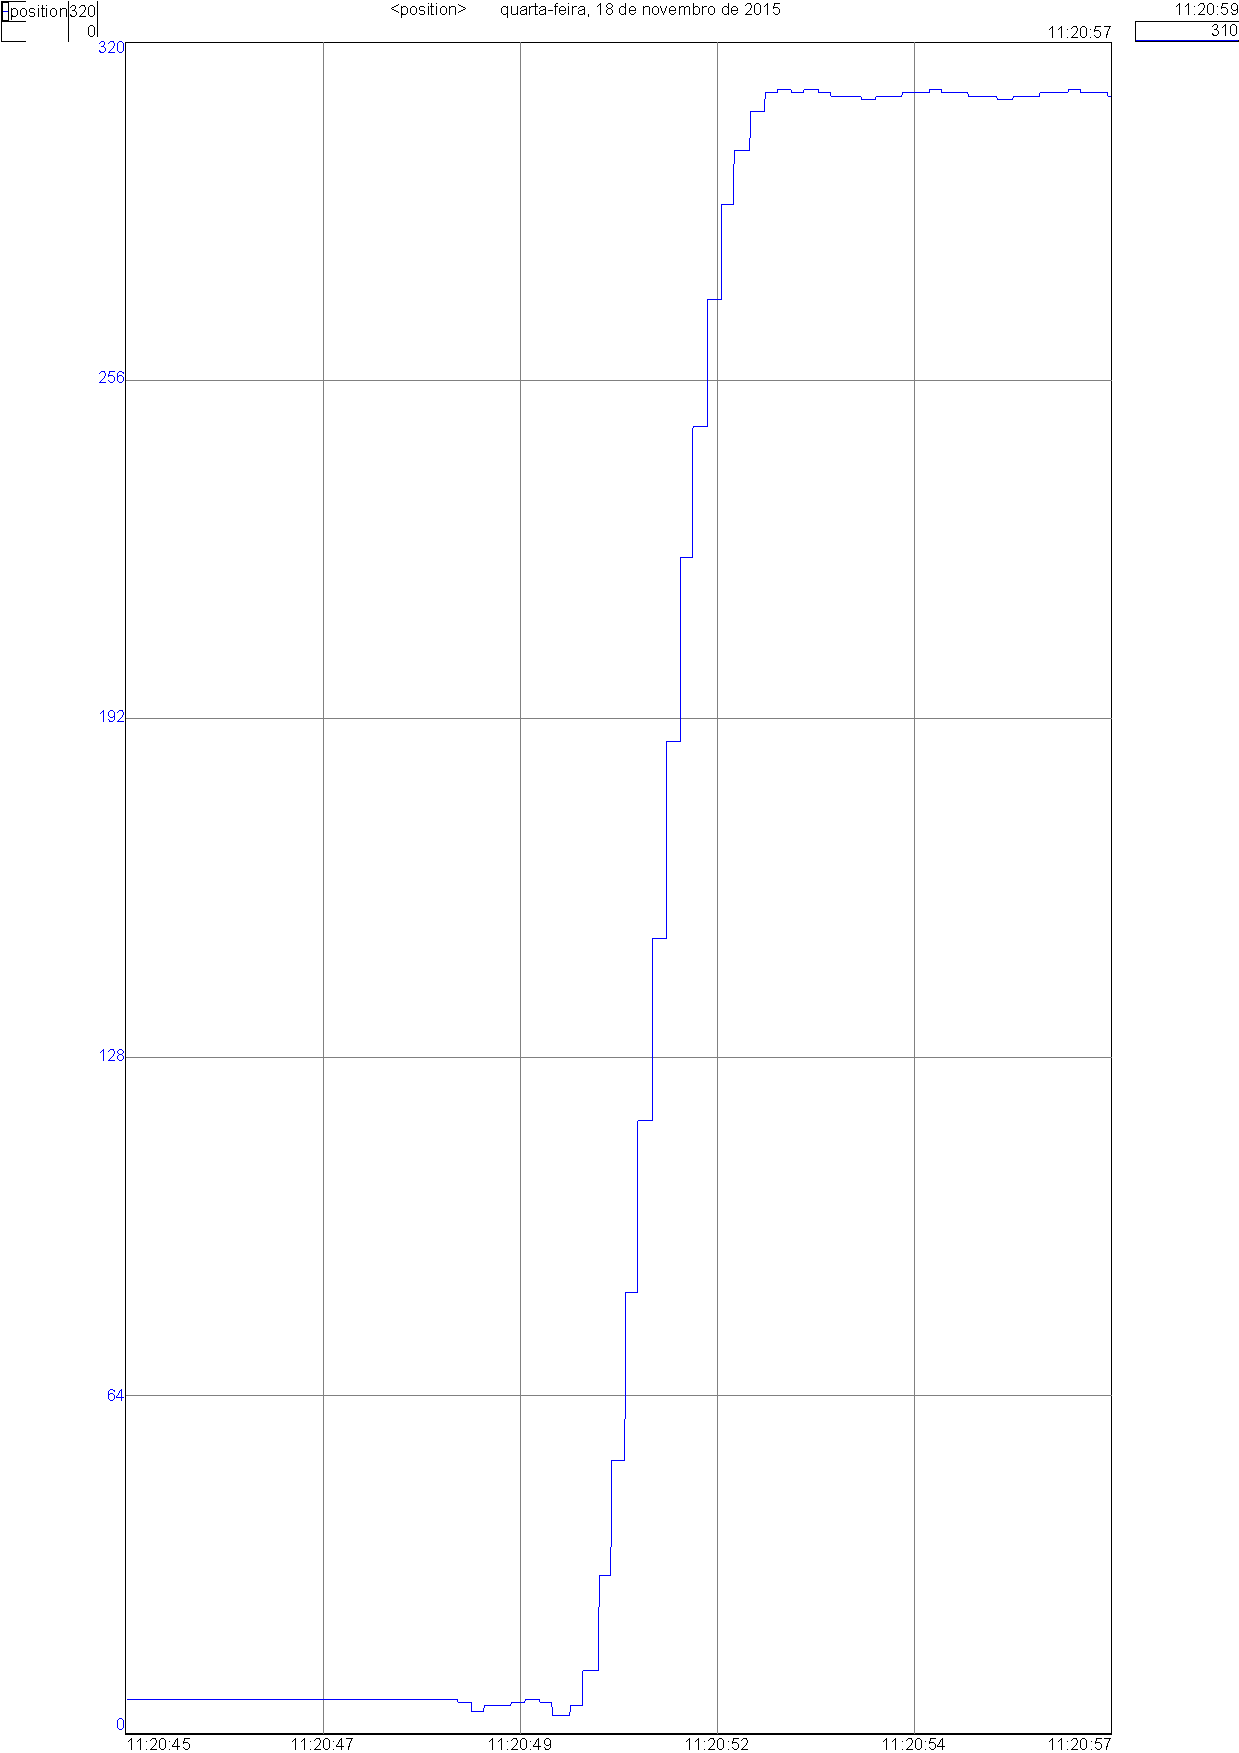
\includegraphics[width=1\linewidth,height=6cm]{figs/resultados/malha_aberta_1/trajetoriaObtidaModelada.pdf}
        \caption{Resultado com Velocidade Modelada para Excursão de 30cm}
        \label{trajetoriaObtidaModelada}
    \end{minipage}%
    \hspace{0.1cm}
    \begin{minipage}{0.45\textwidth}
        \centering
        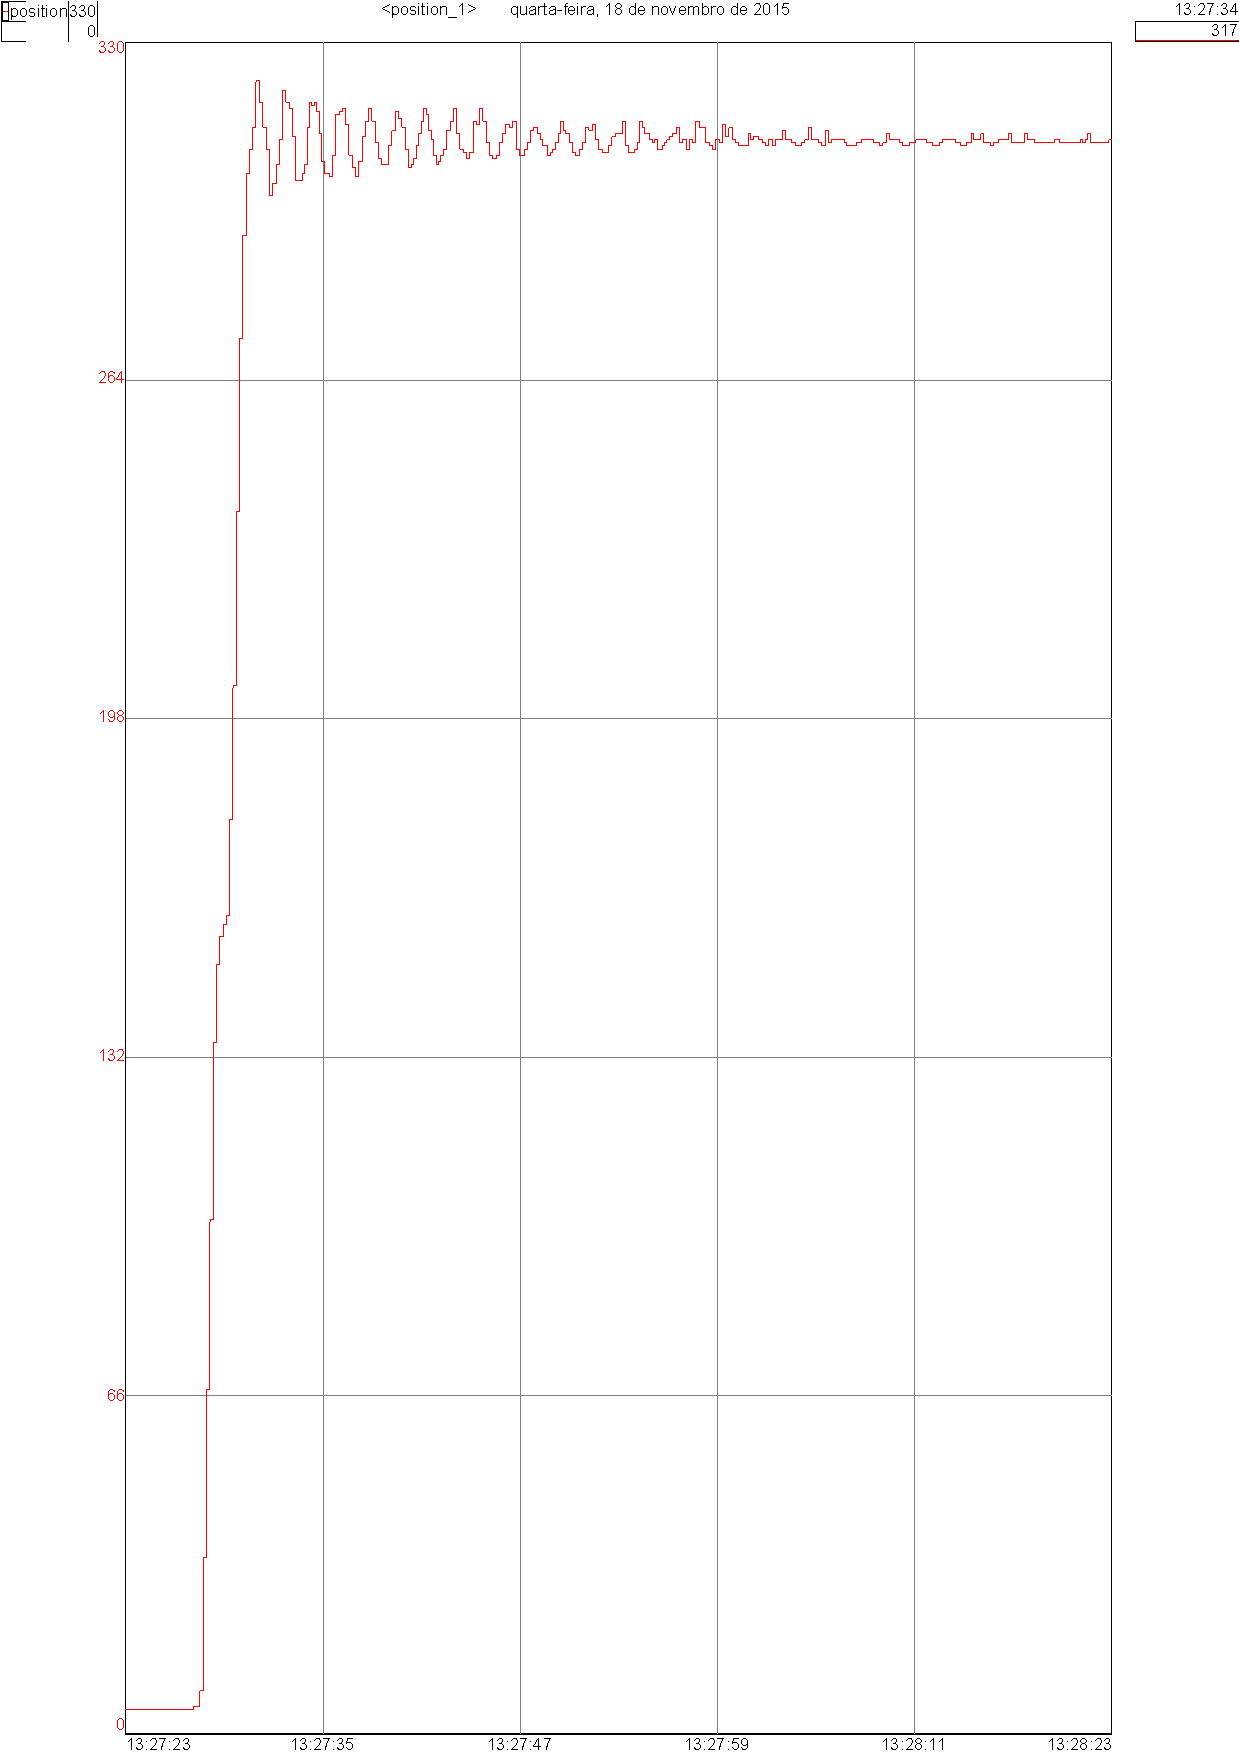
\includegraphics[width=1\linewidth,height=6cm]{figs/resultados/malha_aberta_1/trajetoriaObtidaVConstante.pdf}
        \caption{Resultado com Velocidade Constante para Excursão de 30cm}
        \label{trajetoriaObtidaVConstante}
    \end{minipage}
\end{figure}

\subsection{Excursão de 20cm}
Na prática, o diâmetro do \textit{riser} e de sua massa é bem menor que o comprimento do mesmo. Daí, é importante testar uma menor excursão. Além disso, esse teste terá menor tempo de movimentação e resultará numa velocidade média maior que o caso anterior. Desta forma, maiores oscilações são esperadas e o controle se torna mais difícil.

A trajetória de posição obtida é apresentada na Figura \ref{DeslocamentoT2} e a sua derivada é apresentada na Figura \ref{VelocidadeT2}. O período da tarefa eventual foi escolhido em $100\mathrm{ms}$. O resultado experimental\footnote{Controle Malha Aberta Modelado, 20cm - \url{https://youtu.be/wg1Wq_6VRSg}. Acesso em 29/11/2015.} apresentou mais oscilações que o caso anterior, mas está bem controlado, conforme se vê na Figura \ref{percurso20cmBom}. O resultado com velocidade constante\footnote{Controle Malha Aberta a Velocidade Constante, 20cm - \url{https://youtu.be/Ges2-eYy69k}. Acesso em 29/11/2015.} está na Figura \ref{percurso20cmRuim} e nota-se que o resultado ficou bem pior. A velocidade média foi cerca de $\overline{v} \approx \frac{200\mathrm{mm}}{1.5\mathrm{s}} = 133.3\mathrm{mm}/\mathrm{s}$.

\begin{figure}[!htb]
    \centering
    \begin{minipage}{.45\textwidth}
        \centering
        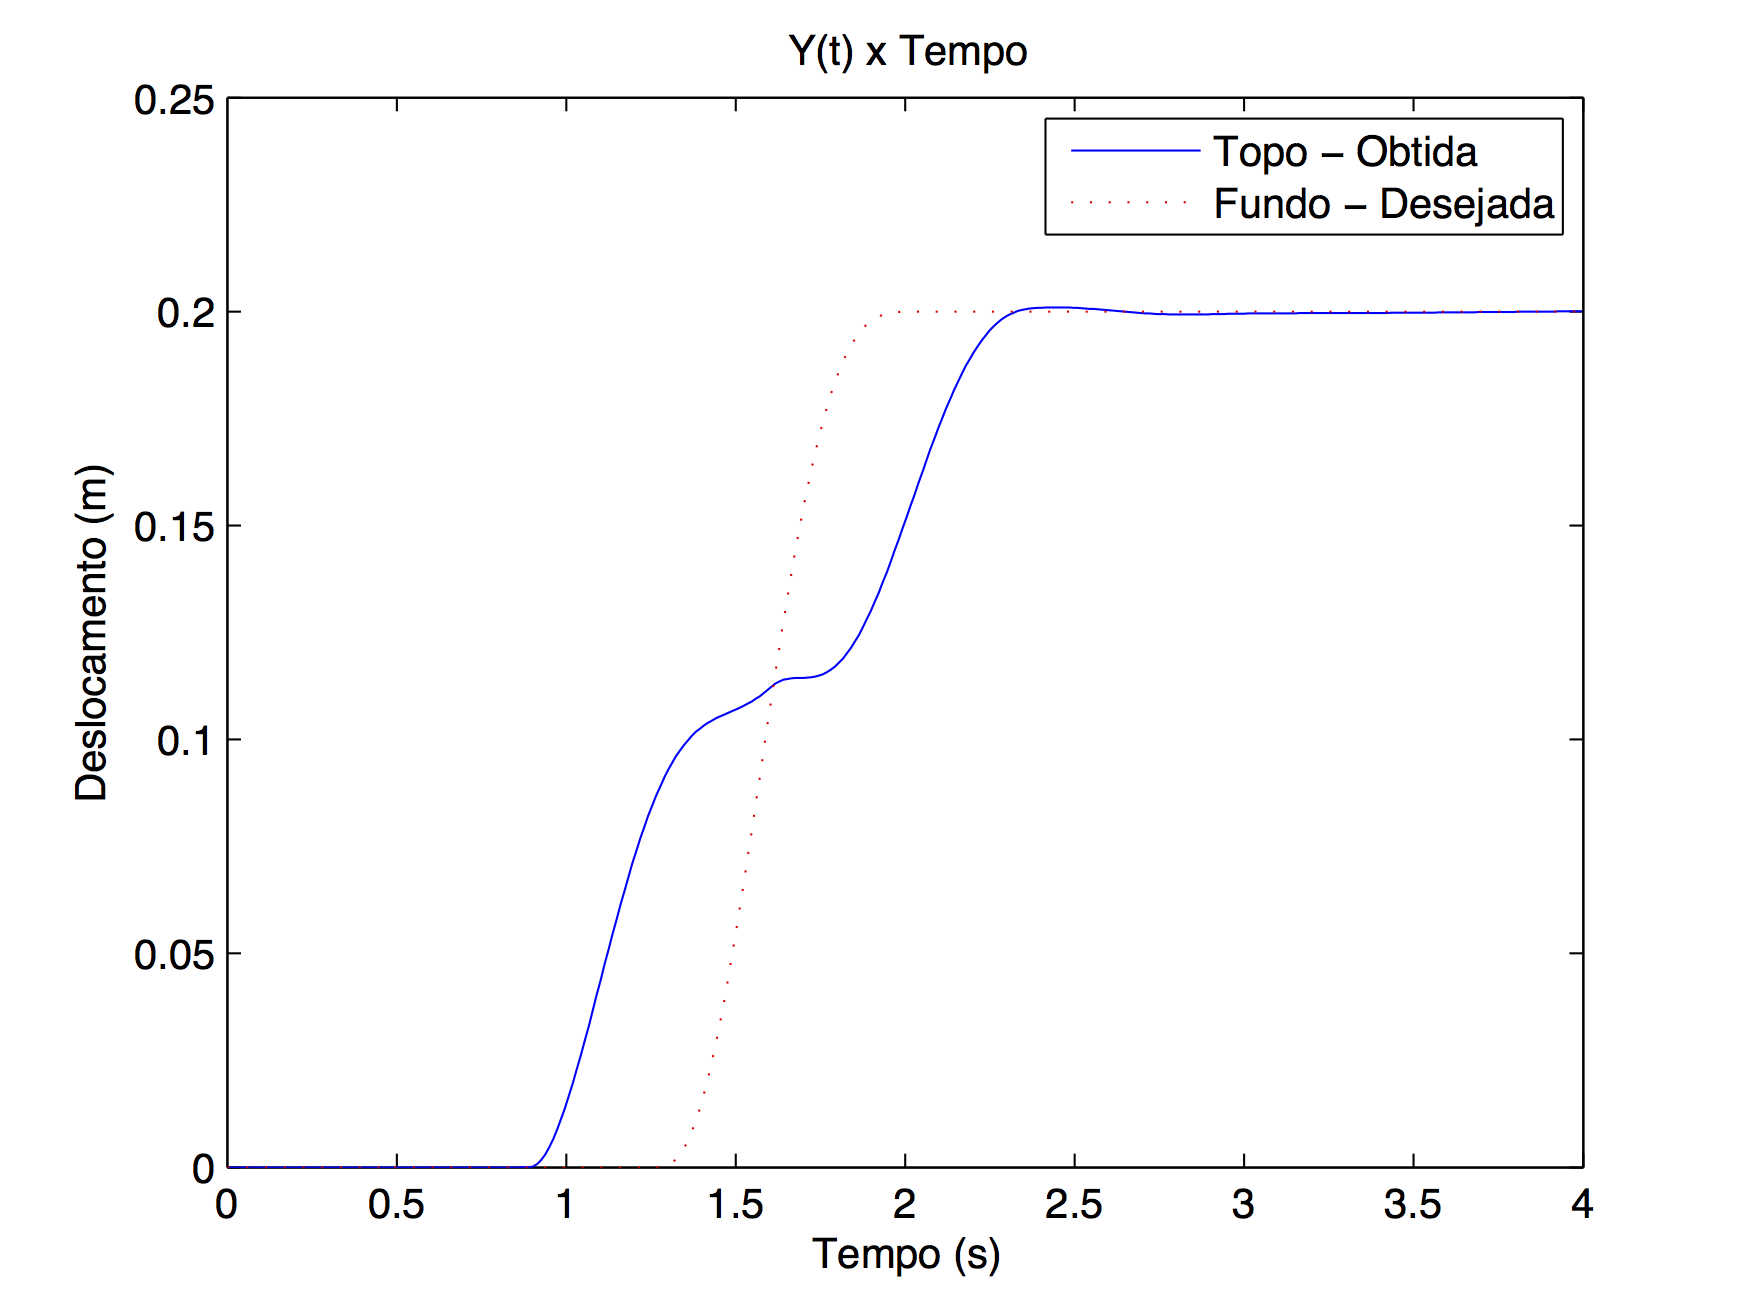
\includegraphics[width=1\linewidth]{figs/resultados/malha_aberta_2/DeslocamentoT2}
        \caption{Referência de Posição para Excursão de 20cm}
        \label{DeslocamentoT2}
    \end{minipage}%
    \hspace{0.1cm}
    \begin{minipage}{0.45\textwidth}
        \centering
        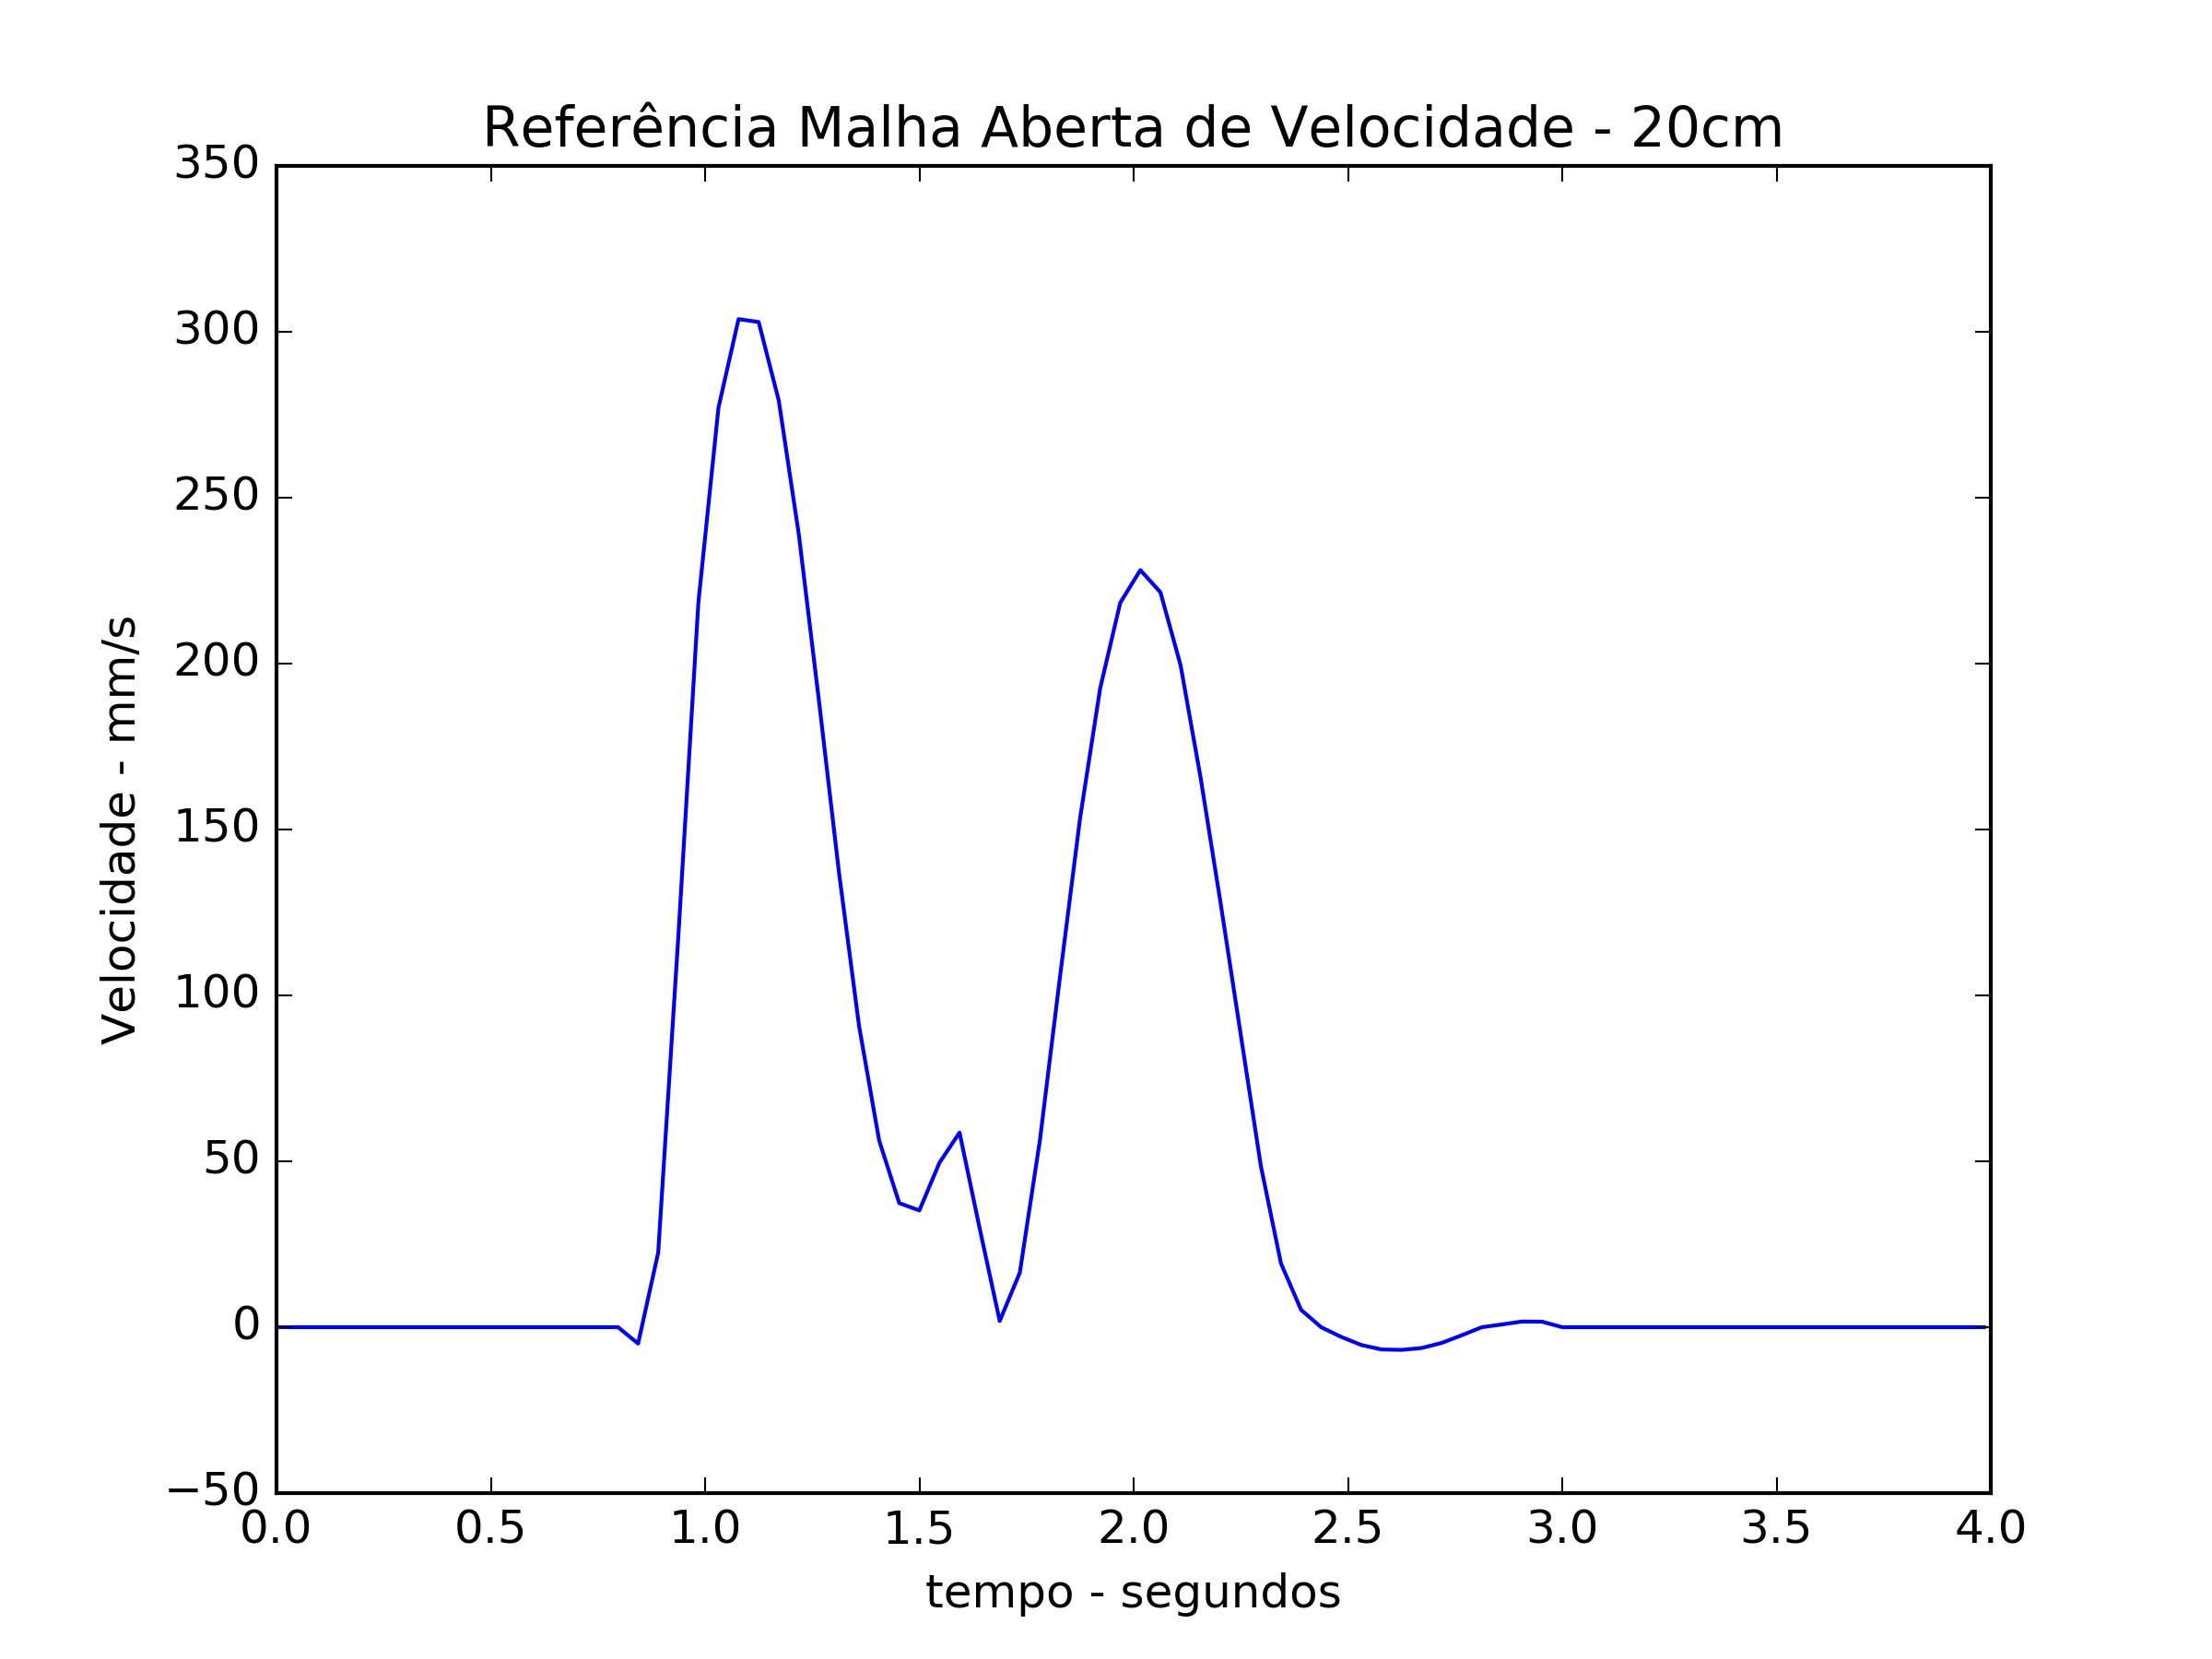
\includegraphics[width=1\linewidth]{figs/resultados/malha_aberta_2/VelocidadeT2}
        \caption{Referência de Velocidade para Excursão de 20cm}
        \label{VelocidadeT2}
    \end{minipage}
\end{figure}

\begin{figure}[!htb]
    \centering
    \begin{minipage}{.45\textwidth}
        \centering
        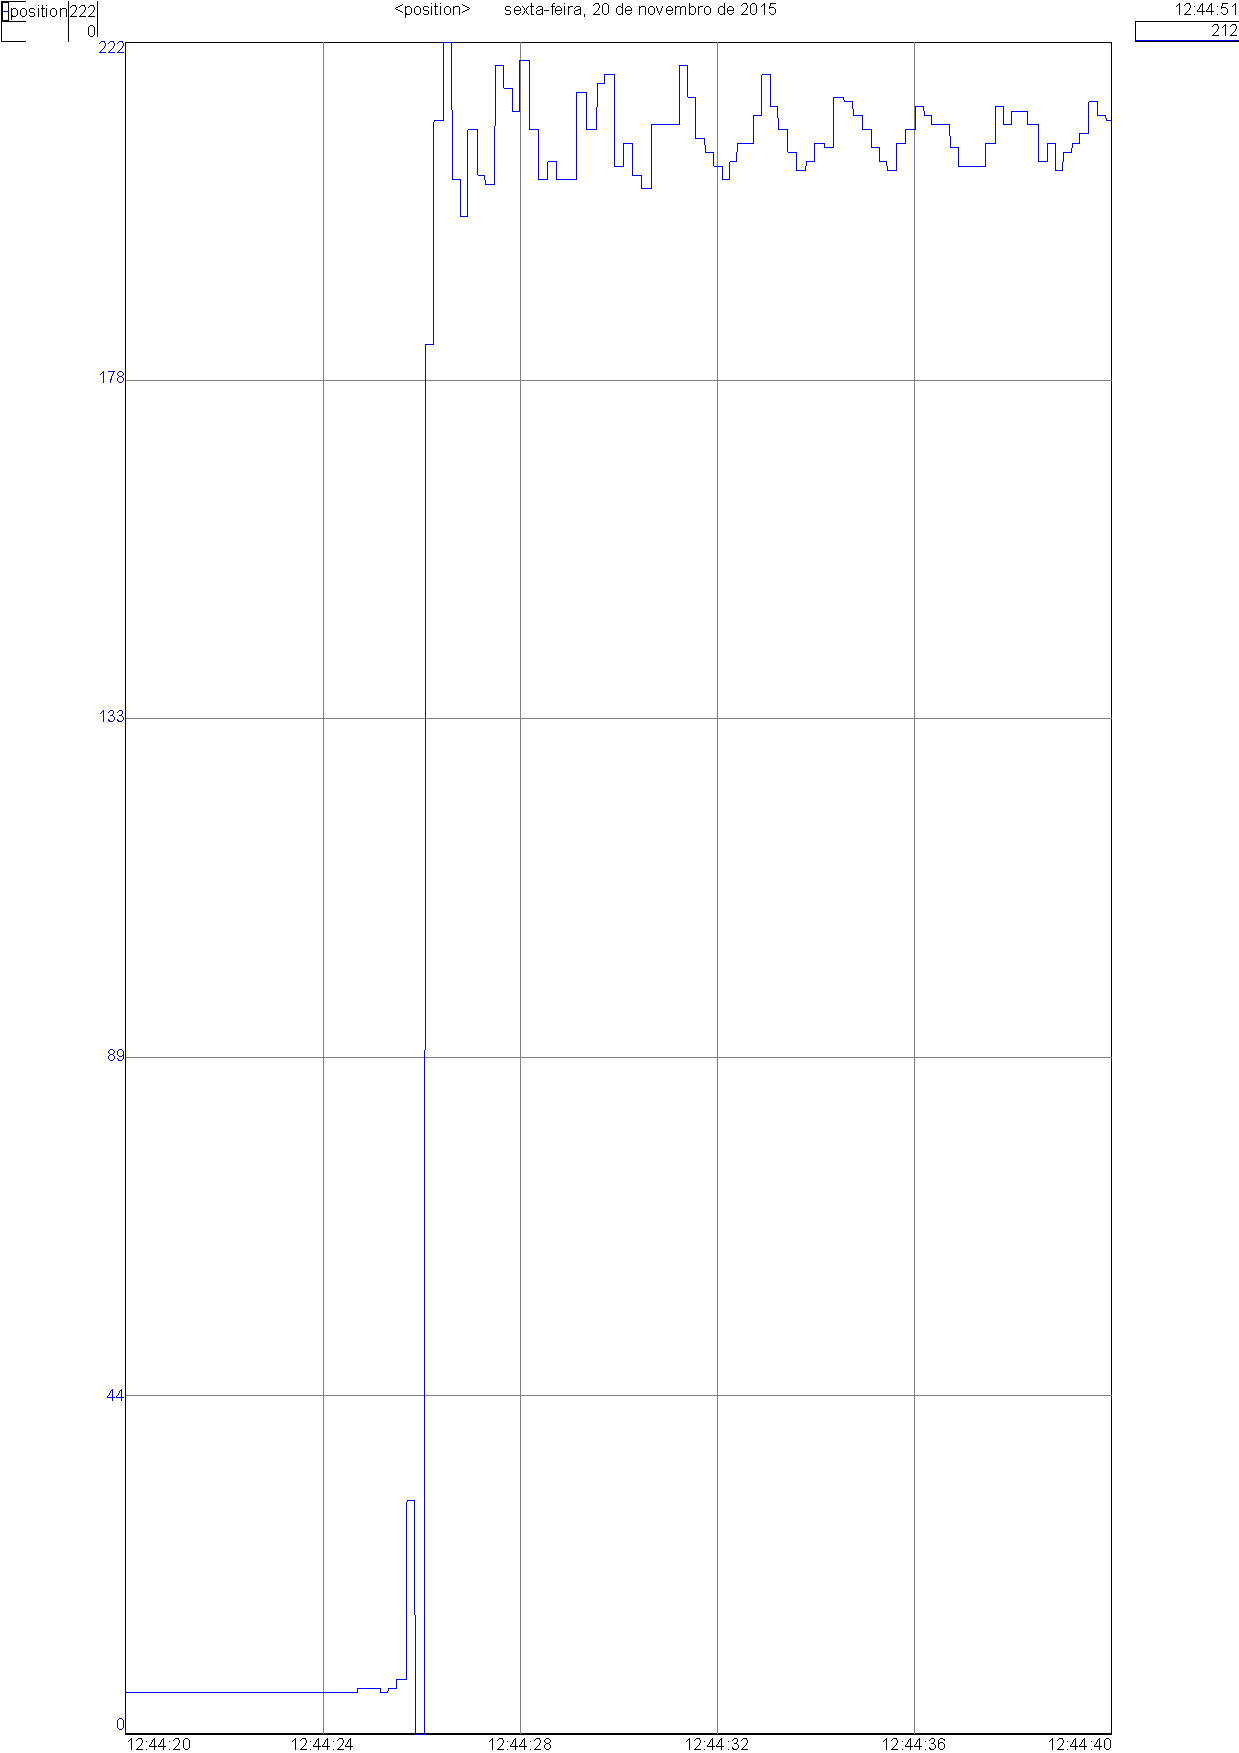
\includegraphics[width=1\linewidth,height=6cm]{figs/resultados/malha_aberta_2/percurso20cmBom.pdf}
        \caption{Resultado com Velocidade Modelada para Excursão de 20cm}
        \label{percurso20cmBom}
    \end{minipage}%
    \hspace{0.1cm}
    \begin{minipage}{0.45\textwidth}
        \centering
        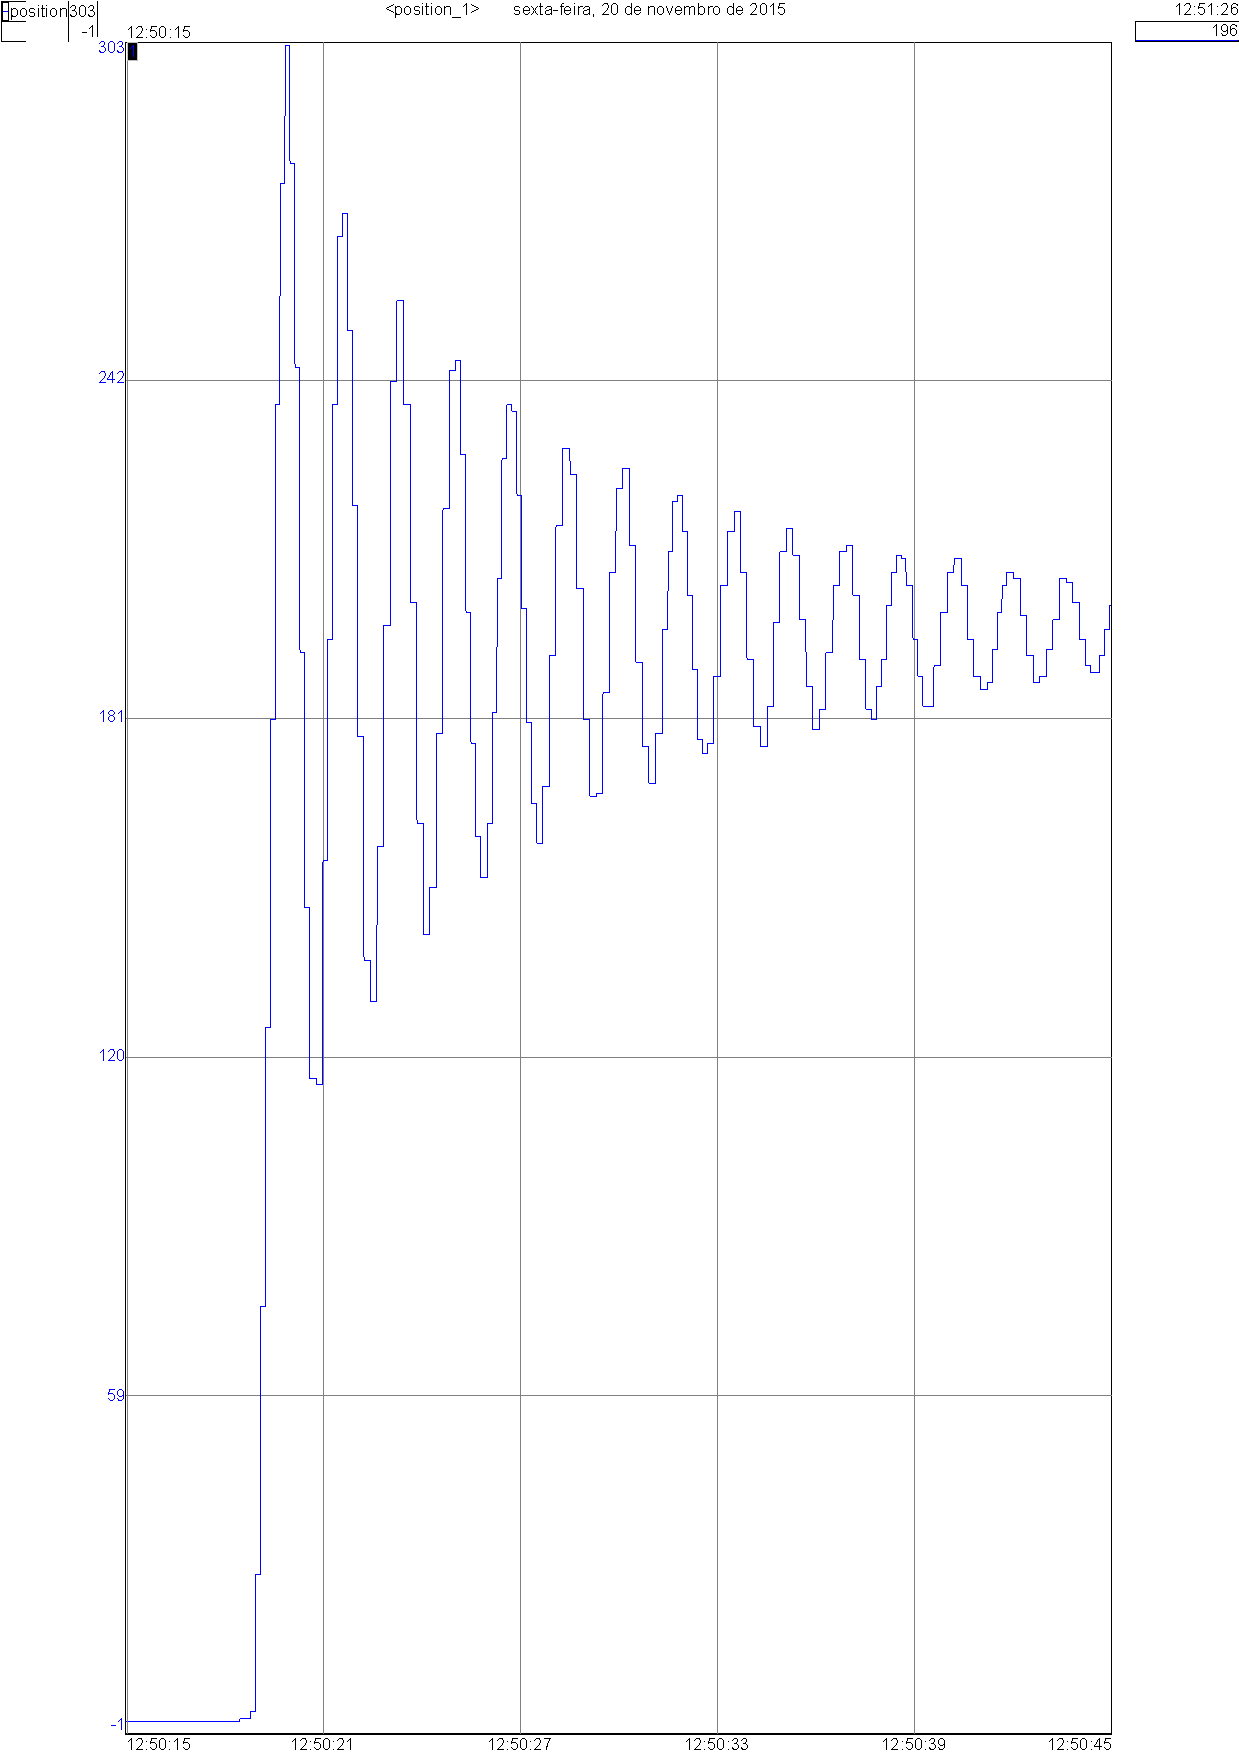
\includegraphics[width=1\linewidth,height=6cm]{figs/resultados/malha_aberta_2/percurso20cmRuim.pdf}
        \caption{Resultado com Velocidade Constante para Excursão de 20cm}
        \label{percurso20cmRuim}
    \end{minipage}
\end{figure}






\section{Malha fechada\label{malhafechadaSection}}
O controle em malha fechada deve ser capaz de compensar por perturbações, pois o sensor identifica o resultado da atuação e realimenta a informação no sistema. Neste trabalho, conseguiu-se configurar a câmera adequadamente e faz-se um teste em malha fechada de um controlador bem simples: um controlador proporcional.

\subsection{Controlador P}

O controlador proporcional utilizado tem o esquema conforme Figura \ref{mfechadaP}. A referência de posição $r = r(t)$ é a entrada do sistema e a saída medida pela câmera, $y_m$, é subtraída da referência para resultar no erro $e$, cuja unidade é dada em milímetros. A entrada da planta, $v$, é dad em $[\mathrm{u}/\mathrm{s}]$, conforme discutido anteriormente na subseção \ref{calibracaoServomotorSecao}. Desta forma, a unidade de $K_p$ é $\left[\frac{\mathrm{u}}{\mathrm{mm}\cdot\mathrm{s}}\right]$.

\begin{figure}[!ht]
\centering
\begin{tikzpicture}[auto, node distance=2cm,>=latex']
% We start by placing the blocks
\node [input, name=input] {};
\node [sum, right of=input] (sum) {};
\node [block, right of=sum] (controller) {$K_p$};
\node [block, right of=controller, pin={[pinstyle]above:Perturbações},
node distance=3cm] (system) {Planta};
% We draw an edge between the controller and system block to 
% calculate the coordinate u. We need it to place the measurement block. 
\draw [->] (controller) -- node[name=u] {$v$} (system);
\node [output, right of=system] (output) {};
\node [block, below of=u] (measurements) {Câmera};

% Once the nodes are placed, connecting them is easy. 
\draw [draw,->] (input) -- node {$r$} (sum);
\draw [->] (sum) -- node {$e$} (controller);
\draw [->] (system) -- node [name=y] {$y$}(output);
\draw [->] (y) |- (measurements);
\draw [->] (measurements) -| node[pos=0.99] {$-$} 
node [near end] {$y_m$} (sum);
\end{tikzpicture}
\caption{Malha fechada de controle\label{mfechadaP}}
\end{figure}

Valores de $K_p$ foram escolhidos empiricamente e o resultado para $K_p = 0.0025$\footnote{Controle Malha Fechada com Kp = 0.0025 - \url{https://youtu.be/mmT1ZwFBJ4s}. Acesso em 29/11/2015.} está na Figura \ref{MFProporcionalKpbaixo} enquanto para $K_p = 0.0050$\footnote{Controle Malha Fechada com Kp = 0.0050 - \url{https://youtu.be/sHh3yvBrek4}. Acesso em 29/11/2015.} está na Figura \ref{MFProporcionalKpmedio}.


\begin{figure}[!htb]
    \centering
    \begin{minipage}{.45\textwidth}
        \centering
        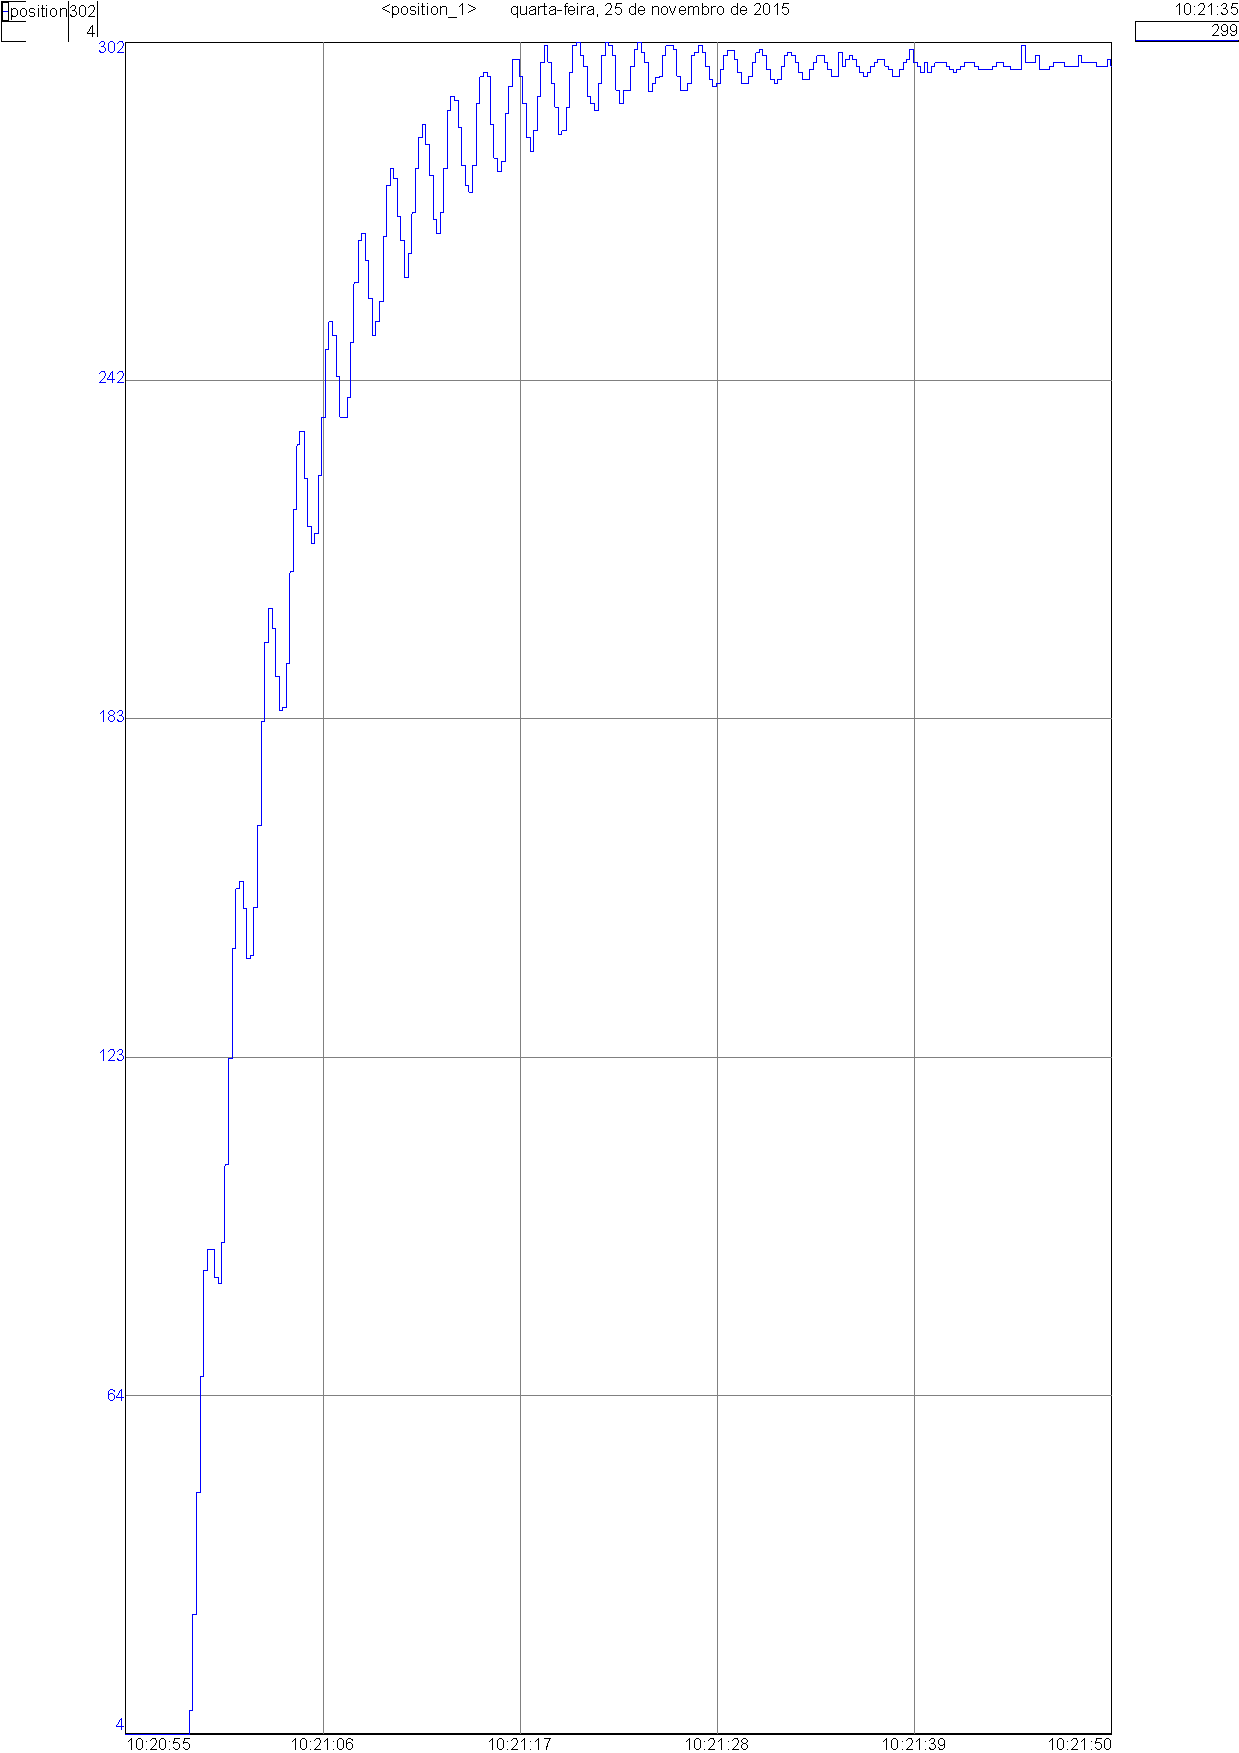
\includegraphics[width=1\linewidth,height=6cm]{figs/resultados/malha_fechada_P/MF_Proporcional_Kp_00025.pdf}
        \caption{Resultado com Malha Fechada Proporcional e $K_p = 0.0025\frac{\mathrm{u}}{\mathrm{mm}\cdot\mathrm{s}}$}
        \label{MFProporcionalKpbaixo}
    \end{minipage}%
    \hspace{0.1cm}
    \begin{minipage}{0.45\textwidth}
        \centering
        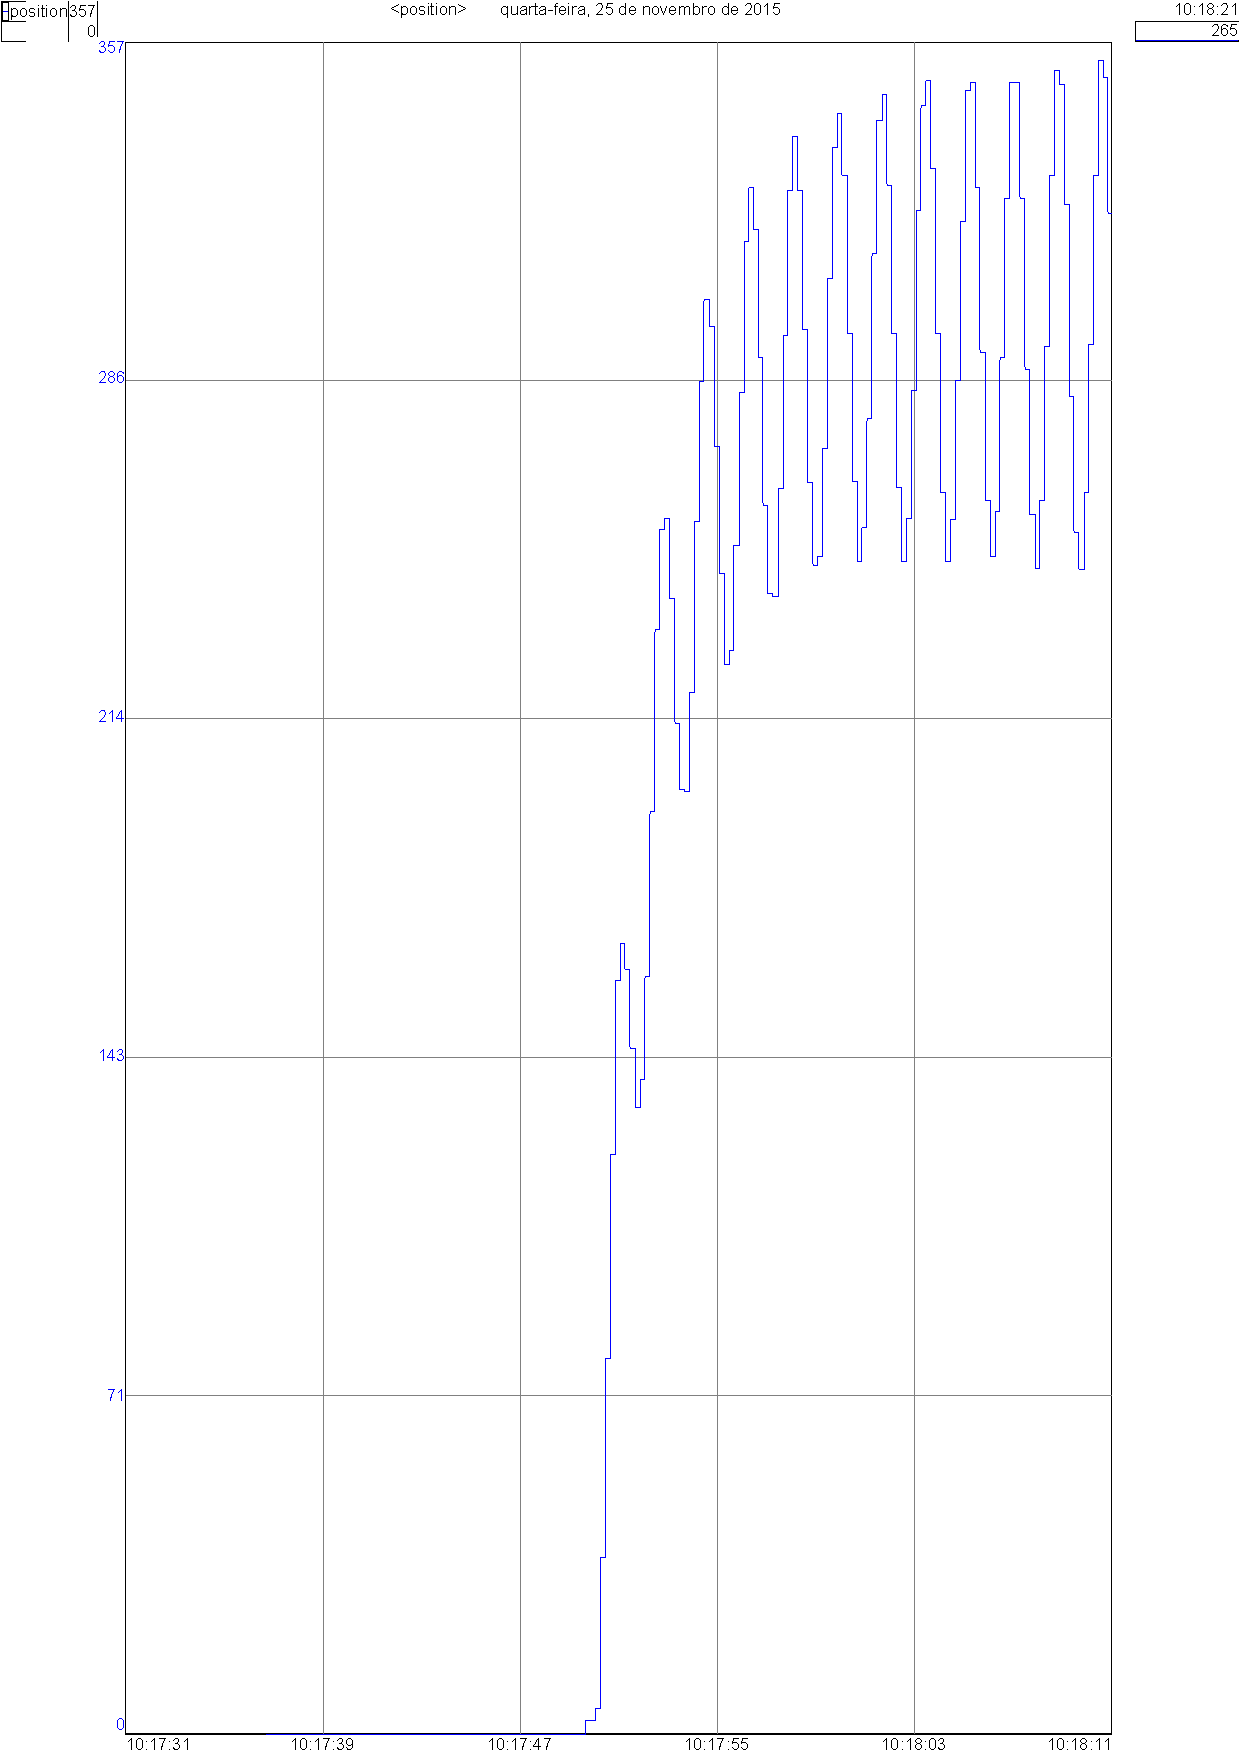
\includegraphics[width=1\linewidth,height=6cm]{figs/resultados/malha_fechada_P/MF_Proporcional_Kp_00050.pdf}
        \caption{Resultado com Malha Fechada Proporcional e $K_p = 0.0050\frac{\mathrm{u}}{\mathrm{mm}\cdot\mathrm{s}}$
        \label{MFProporcionalKpmedio}}
    \end{minipage}
\end{figure}

O período de amostragem utilizado foi de $100\mathrm{ms}$ e o ar condicionado estava ligada nas duas situações apresentadas e nota-se que o primeiro resultado é bem melhor que o primeiro, tendo menos oscilações. No entanto, este resultado está aquém do obtido em malha aberta.



%Conclusões
%TCIDATA{LaTeXparent=0,0,relatorio.tex}



\chapter{Conclusões}

\label{CapConclusoes}

O projeto desenvolvido até aqui é uma continuação do que foi desenvolvido por Rédytton \cite{redytton}; porém, muitos avanços foram realizados. Em primeiro lugar, na primeira parte do projeto, foram melhorados aspectos relativos ao que foi previamente realizado, como por exemplo:
\begin{itemize}
\item Foi efetuada uma calibração da câmera, de forma a se pegar os dados da trajetória de fundo, representada pela bolinha;
\item Foi calculado um fator de conversão entre a unidade de velocidade reconhecida pelo RsLogix e uma unidade de velocidade derivada do SI --- milímetros por segundo;
\item Foi adotado o texto estruturado para se desenvolver as estratégias de controle a serem realizadas pelo CLP, uma vez que o texto é facilmente reprogramável para novas trajetórias, o que não ocorre com linguagens gráficas como o \textit{ladder};
\item Foi modificado o protocolo de comunicação do CLP com o computador. O novo protocolo, Ethernet/IP, é consideravelmente mais rápido que uma comunicação baseada em RS-232, o que resulta em um tempo menor entre um teste e outro;
\item Um último avanço foi o uso do OPC. Dessa forma, uma estrutura complexa como o preditor de Smith pode ser programada em uma linguagem mais rica em termos de ferramentas do que o texto estruturado --- no caso, foi utilizada a linguagem Python com o módulo OpenOPC \cite{OpenOPC}.
\end{itemize}

No início do trabalho, não havia nenhum conhecimento prévio dos autores sobre programação em tempo real utilizando CLPs; os conhecimentos de programação CLP em geral eram bastante limitados. Além disso, nenhum conhecimento prévio da bancada existia também. No estágio atual, pode-se dizer que há relevante facilidade em se trabalhar com a bancada, apesar de não se ter entrado em detalhes de como funciona o servomotor, \textit{drive} e outros componentes.

O foco do projeto era desenvolver uma estrutura de controle não clássico para lidar com um sistema de ordem infinita, representado pelo conjunto carrinho, bolinha e barbante. Dentro dessa abordagem, procurou-se validar, por meio de um extenso tratamento matemático, o experimento de forma a ele representar, confiavelmente, uma operação de re-entrada com um \textit{riser} real. Dada a estratégia de redução modal de forma a se obter um espaço de estados com uma ordem tal que fosse razoavelmente elementar desenvolver uma estratégia de controle simples, como o de realimentação de estados com canal integral, buscou-se, através do uso do preditor de Smith com Filtro de Kalman, controlar a planta de tal forma que a trajetória de fundo real acompanhasse sua referência com erro mínimo, mesmo na presença de perturbações.

Embora os resultados experimentais não terem sido ideais, pode-se notar que o uso do preditor de Smith é um grande avanço em relação ao teste com malha aberta no que concerne ao acompanhamento da trajetória; porém, considerando todas as fontes de erro oferecidas pela planta em questão --- posicionamento da câmera, perdas de comunicação entre câmera, CLP e computador, atrito na esteira do carrinho, conversão de velocidades, atraso devido à comunicação (\textit{overhead}), entre outros fatores ---, nota-se que os resultados foram satisfatórios; em outras palavras, pode-se dizer que é válido o uso do preditor de Smith como estratégia de controle para uma operação de re-entrada de \textit{risers}, tendo como base os resultados encontrados.


\section{Perspectivas Futuras}
Embora os resultados apresentados até aqui sejam satisfatórios, há muito a ser feito. Além do foco em reduzir o erro em muitos dispositivos da planta, particularmente na câmera, há outros pontos de melhoria no projeto, como por exemplo:
\begin{itemize}
\item Utilizar uma estratégia de calibração da câmera melhor --- a atual não permite excursões maiores que 50 cm;
\item Estudar outras formas de controle para o \textit{riser}, e verificar o desempenho das mesmas em relação ao preditor de Smith;
\item Procurar melhorar a programação, otimizando os algoritmos desenvolvidos e utilizando ferramentas para acelerar os programas já feitos (por exemplo, o uso de \textit{threads}, já feito neste projeto). A razão de se acelerar os programas que fazem a comunicação com por meio do OPC é impedir que seus custos de execução e \textit{overheads} interfiram no tempo de amostragem, comprometendo os resultados;
\item Fazer testes mais minuciosos com as estruturas já desenvolvidas, e utilizar Filtros de Kalman diferentes (por exemplo, filtros adaptativos). O objetivo aqui é atenuar ainda mais as perturbações que venham a ocorrer, visto que um \textit{riser} real é constantemente atingido por forças externas ao controle, como correntes maritmas e eventuais colisões com outros corpos.
\end{itemize}



%Bibliografia

\renewcommand{\bibname}{REFERÊNCIAS BIBLIOGRÁFICAS} 
\addcontentsline{toc}{chapter}{REFERÊNCIAS BIBLIOGRÁFICAS} 

\bibliographystyle{abnt-num}
\bibliography{relatorio}

%
\anexos 
\makeatletter 
%% não retirar estes comandos 
\renewcommand{\@makechapterhead}[1]{%
  {\parindent \z@ \raggedleft \setfontarial\bfseries          
\LARGE \thechapter. \space\space      
\uppercase{#1}\par     
\vskip 40\p@   
} 
} 
\makeatother
%
%%Anexo I: Descriçao do CD
%
%%TCIDATA{LaTeXparent=0,0,relatorio.tex}



\chapter{Descrição do conteúdo do CD}

\label{AnCD} 

Descrever CD.

%
%\refstepcounter{noAnexo}
%
% %Anexo II: Programas Utilizados


%TCIDATA{LaTeXparent=0,0,relatorio.tex}



\chapter{Programas utilizados}

\section{Texto Estruturado}
\label {stsection}

\subsection{Inicialização do primeiro teste de malha aberta}
\label {stMAinit1}
\lstinputlisting{codes/init1.st}

\subsection{Inicialização do segundo teste de malha aberta}
\label {stMAinit2}
\lstinputlisting{codes/init2.st}

\subsection{Inicialização dos testes de malha fechada}
\label {stMFinit}
\lstinputlisting{codes/initP.st}

\subsection{Inicialização da rede DeviceNET}
\label{}

\section{Linguagem \textit{ladder}}

\section{Programas da câmera}
\subsection{Detecção da posição horizontal da bolinha}
\label{ballhorzpos}
\begin{figure}[!ht]
\centering
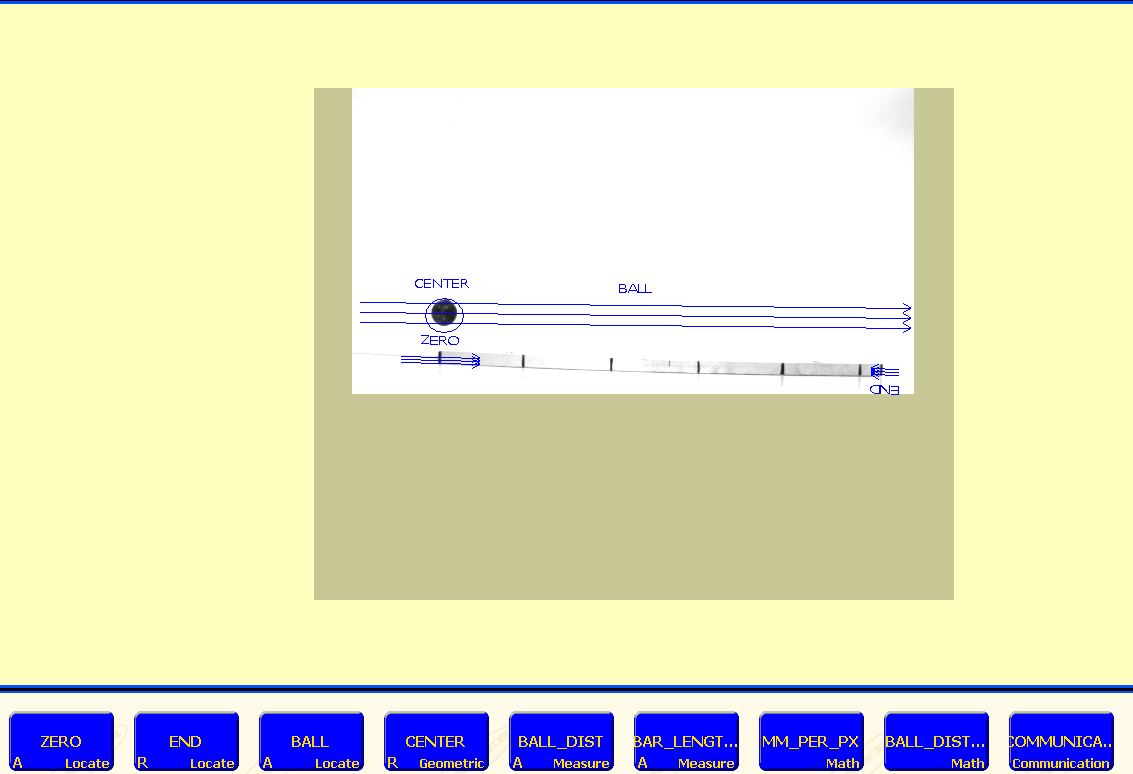
\includegraphics[width=\linewidth]{figs/presence/programaCaptura}
\caption{Detecção da posição horizontal da bolinha}
\end{figure}
\refstepcounter{noAnexo}

%%Acrescente mais anexos conforme julgar necessário.

\end{document}
